%% uctest.tex 11/3/94
%% Copyright (C) 1988-2004 Daniel Gildea, BBF, Ethan Munson.
%
% This work may be distributed and/or modified under the
% conditions of the LaTeX Project Public License, either version 1.3
% of this license or (at your option) any later version.
% The latest version of this license is in
%   http://www.latex-project.org/lppl.txt
% and version 1.3 or later is part of all distributions of LaTeX
% version 2003/12/01 or later.
%
% This work has the LPPL maintenance status "maintained".
% 
% The Current Maintainer of this work is Daniel Gildea.
%
% 2007/08/01
% LaTeX Package "ucr" is modified from LaTeX package "ucthesis."
% This modification is therefore under to the conditions of 
% the LaTeX Project Public License.
% Its formality is suitable for the dissertation of Universty of
% California, Riverside.
% This test document is for the convenience of all students of
% Universty of California, Riverside.
% Contact Charles Yang at chcyang@yahoo.com if you like.
% Charles Yang has nothing to do with the original author's sarcasm.
%
%%%%%%%%%%%%%%%%%%%%%%%%%%%%%%%%%%%%%%%%%%%%%%%%%%%%%%%%%%%%%%%%%%%%%%%%%%%%%%%%%
%% Document: Thesis for PhD at UC Riverside                                    %%
%% Title: Investigating the evolution of environmental and biotic interactions %% 
%%          in basal fungal lineages through comparative genomics              %%
%% Author: Steven Ahrendt                                                      %%
%%%%%%%%%%%%%%%%%%%%%%%%%%%%%%%%%%%%%%%%%%%%%%%%%%%%%%%%%%%%%%%%%%%%%%%%%%%%%%%%%
% \documentclass[11pt]{ucthesis}
\documentclass[11pt]{UCR_latex_template/ucr}
%\documentclass[oneside,final,letter]{ucr}
\usepackage{anysize}
\usepackage[left=1.5in,top=1.5in,right=1in,bottom=1in]{geometry}
% \usepackage{bm}
% \usepackage{mathrsfs}
% \usepackage[dvips]{graphicx}
% \usepackage{graphics}
% \usepackage{subfigure}
% \usepackage{flafter}
% \usepackage{sw20uctd}
\usepackage{xspace}
\usepackage{graphicx}
\usepackage{Styles/pdfsync}
\usepackage{amsmath}
% \usepackage{amssymb}
% \usepackage{amsthm}
% \usepackage{fancyhdr} 
\usepackage{fncylab}
\usepackage[usenames]{color}
% \usepackage{enumerate}
% \usepackage{multirow}
% \usepackage{setspace}

%%---------------
%% Packages added by Steven Ahrendt
%%-----------//
\usepackage{url} % use with \url{} for formatted urls; nonclickable
\usepackage[graphicx]{realboxes}
\usepackage{texshade}
\usepackage{booktabs}  % Added to make
\usepackage{longtable}
\makeatletter
\g@addto@macro\@floatboxreset\centering
\makeatother
\usepackage{lscape}
\usepackage{multirow}
\usepackage[english]{babel}      % for proper formatting of 
\usepackage[autostyle]{csquotes} % quotemarks
\usepackage{fancyvrb} % for including fasta file with \VerbatimInput
%% These five lines correct issues with longtable caption format
\usepackage[font=small]{caption}[2013/02/03]
\AtBeginEnvironment{longtable}{\linespread{1}\selectfont}
\setlength{\LTcapwidth}{\linewidth}
\AtBeginEnvironment{table}{\linespread{1}\selectfont}
\AtBeginEnvironment{figure}{\linespread{1}\selectfont}
%%-------------------------------------//

\setcounter{secnumdepth}{3}
\setcounter{tocdepth}{3}

%\newtheorem{theorem}{Theorem}
%\newtheorem{acknowledgement}[theorem]{Acknowledgement}
%\newtheorem{algorithm}[theorem]{Algorithm}
%\newtheorem{axiom}[theorem]{Axiom}
%\newtheorem{case}[theorem]{Case}
%\newtheorem{claim}[theorem]{Claim}
%\newtheorem{conclusion}[theorem]{Conclusion}
%\newtheorem{condition}[theorem]{Condition}
%\newtheorem{conjecture}[theorem]{Conjecture}
%\newtheorem{corollary}[theorem]{Corollary}
%\newtheorem{criterion}[theorem]{Criterion}
%\newtheorem{definition}[theorem]{Definition}
%\newtheorem{example}[theorem]{Example}
%\newtheorem{exercise}[theorem]{Exercise}
%\newtheorem{lemma}[theorem]{Lemma}
%\newtheorem{notation}[theorem]{Notation}
%\newtheorem{problem}[theorem]{Problem}
%\newtheorem{proposition}[theorem]{Proposition}
%\newtheorem{remark}[theorem]{Remark}
%\newtheorem{solution}[theorem]{Solution}
%\newtheorem{summary}[theorem]{Summary}
%\newtheorem{observation}[theorem]{Observation}
\newenvironment{proof}[1][Proof]{\textbf{#1.} }{\ \rule{0.5em}{0.5em}}
\def\dsp{\def\baselinestretch{2.0}\large\normalsize}
\dsp

%TCIDATA{OutputFilter=LATEX.DLL}
%TCIDATA{Created=Saturday, April 29, 2006 22:07:22}
%TCIDATA{LastRevised=Tuesday, July 17, 2007 22:48:56}
%TCIDATA{<META NAME="GraphicsSave" CONTENT="32">}
%TCIDATA{<META NAME="DocumentShell" CONTENT="Other Documents\SW\Thesis - University of California Thesis">}
%TCIDATA{Language=American English}
%TCIDATA{CSTFile=ucr.cst}


%% tcilatex is a package from Scientific Workplace.
%% The user may remove the following line without serious damage.
%% \input{tcilatex}


\usepackage{Sweave}
\begin{document}
%%%%%%%%%%%%%%
% TITLE PAGE %
%%%%%%%%%%%%%%

% Declarations for Front Matter

\title{Investigating the Evolution of Environmental and Biotic Interactions in \\Basal Fungal Lineages Through Comparative Genomics}
\author{Steven Robert Ahrendt}
\degreemonth{August}
\degreeyear{2015}
\degree{Doctor of Philosophy}
\chair{Dr. Jason E. Stajich }
\othermembers{Dr. Chia-en A. Chang\\
Dr. Katherine A. Borkovich}
\numberofmembers{3}
\field{Genetics, Genomics, and Bioinformatics}
\campus{Riverside}

\maketitle
\copyrightpage{}
\approvalpage{}

\degreesemester{Summer}

\begin{frontmatter}
%%%%%%%%%%%%%%%%%%%%
% ACKNOWLEDGEMENTS %
%%%%%%%%%%%%%%%%%%%%
\begin{acknowledgements}
There are many people to whom I am deeply indebted for their contribution to this dissertation and to whom I would like to extend my appreciation. First and foremost, to my research advisor and mentor Dr. Jason Stajich, who allowed me both the freedom and guidance necessary to see this research to completion. To my co-advisor, Dr. Chia-en Angelina Chang, whose input and assistance helped provide a fresh perspective on aspects of this research. And to Dr. Katherine Borkovich, for her support, guidance, and technical expertise. To my undergraduate internship research advisor Dr. Jamie Foster at the Kennedy Space Center and her graduate student Jen, without whose inspiration, advice, and continued support I would never have pursued graduate school at all. I would like to extend a huge thank you to the members of the Stajich and Chang labs, and especially to the undergraduate students I mentored for their assistance; also to the members of the Borkovich lab, whose equipment and expertise I borrowed early and often. To my parents, for their constant support and continued patience. And finally to Kat, who joined me on the journey and stayed with me until the end, for which I am eternally grateful.\\
\indent The text of this dissertation, in part or in full, is a reprint of the material as is appears in \enquote{Shared Signatures of Parasitism and Phylogenomics Unite Cryptomycota and Microsporidia}, \emph{Current Biology}, 2013.  The co-author, Dr. Jason Stajich, listed in that publication directed and supervised the research which forms the basis for this dissertation.\\
% Funding provided by the University of California, Riverside, and by the Alfred P. Sloan foundation.\\
\end{acknowledgements}

%%%%%%%%%%%%%%
% DEDICATION %
%%%%%%%%%%%%%%
%\begin{dedication}
%\null\vfil
%{\large
%\begin{center}
%For Ruby.
%\end{center}}
%\vfil\null
%\end{dedication}

%%%%%%%%%%%%%%%%%%%%%%%%%%%
% ABSTRACT                %
% Include in abstract.tex %
%%%%%%%%%%%%%%%%%%%%%%%%%%%
%%%%%%%%%%%%%%%%%%%%%%%%%%%%%%%%%%%%%%%%%%%%%%%%%%%%%%%%%%%%%%%%%%%%%%%%%%%%%%%%%
%% Document: Thesis for PhD at UC Riverside                                    %%
%% Title: Investigating the evolution of environmental and biotic interactions %%
%%          in basal fungal lineages through comparative genomics              %%
%% Author: Steven Ahrendt                                                      %%
%%%%%%%%%%%%%%%%%%%%%%%%%%%%%%%%%%%%%%%%%%%%%%%%%%%%%%%%%%%%%%%%%%%%%%%%%%%%%%%%%
% ABSTRACT %
%%%%%%%%%%%%
\begin{abstract}
Species belonging to the early diverging fungal lineages (Blastocladiomycota, Chytridiomycota, Cryptomycota, and Neocallimastigomycota) reproduce via motile uniflagellated zoospores. These organisms are traditionally understudied, despite being active decomposers, parasites, and symbionts with other organisms in the ecosystem. This dissertation research uses a comparative approach to answer questions about how these organisms interact with their environment, regarding potential antifungal and competitive behavior and its mechanisms (Chapter~\ref{chap:HpInhibition}), putative photoreception (Chapters~\ref{chap:RhodStruct} and \ref{chap:RhodAux}), transcriptome analysis of one member of the only known insect associate genus (Chapter~\ref{chap:ClatTranscriptome}), and molecular aspects of the evolutionary transition from aquatic motile single cells to terrestrial multicellullar organisms (Appendix~\ref{app:Flagella}).
\end{abstract}


%%%%%%%%%%%%%%%%%%%%%
% TABLE OF CONTENTS %
%%%%%%%%%%%%%%%%%%%%%
\tableofcontents
\listoffigures
\listoftables
\end{frontmatter}

% \part{First Part}


%%%%%%%%%%%%%%%%
% INTRODUCTION %
%%%%%%%%%%%%%%%%
%%%%%%%%%%%%%%%%%%%%%%%%%%%%%%%%%%%%%%%%%%%%%%%%%%%%%%%%%%%%%%%%%%%%%%%%%%%%%%%%%
%% Document: Thesis for PhD at UC Riverside                                    %%
%% Title: Investigating the evolution of environmental and biotic interactions %%
%%          in basal fungal lineages through comparative genomics              %%
%% Author: Steven Ahrendt                                                      %%
%%%%%%%%%%%%%%%%%%%%%%%%%%%%%%%%%%%%%%%%%%%%%%%%%%%%%%%%%%%%%%%%%%%%%%%%%%%%%%%%%
% INTRODUCTION %
%%%%%%%%%%%%%%%%
\chapter{Introduction to the Basal Fungal lineages}
\section{Overview of fungal phylogenetics and the importance of the basal lineages}
%%%%%
% Fungal phylogenetics
%%%%%
The Fungi are one of the major kingdoms of eukaryotic life on
Earth. Various studies have attempted to estimate the date of the
emergence of the Kingdom Fungi \cite{Taylor2006}, when it diverged
from the metazoan lineages. These studies place this occurance at
approximately 1 billion years ago, with a range of around $\pm$500
MYA: 600 MYA \cite{Berbee1993}, 965 MYA \cite{Doolittle1996}, and 1.6
BYA \cite{Wang1999}. These loose approximations are based on
correlation between evolutionary events in fungi and in other
organisms, and are under continued re-evaluation and refinement
\cite{Berbee2010}.\\
\indent A comprehensive review of a collection of 21st century
phylogenetic studies \cite{Hibbett2007} proposes that the Fungal
Kingdom comprises seven phyla: Microsporidia, Chytridiomycota,
Blastocladiomycota, Neocallimastigomycota, Glomeromycota,
Basidiomycota, and Ascomycota, with the most recent inclusion of the
phylum Cryptomycota \cite{Jones2011}.\\
\indent The most recently diverged fungal phyla are the Ascomycota and
Basidiomycota, and together make up the subkingdom Dikarya. This
subkingdom is so named because its members undergo cell fusion
(plasmogamy) without nuclear fusion (karyogamy) during sexual
development, resulting in cells with nuclei from individual parents
("dikaryons"). These organisms are muticellular, with terrestrial
habitats, sexual and asexual life cycle components, and filamentous
growth structures. Collectively, the Dikarya is the most widely
studied group and is home to several model and non-model organisms of
research interest, including the model filamentous Ascomycete
\textit{Neurospora crassa}, the economically critical
\textit{Saccharomyces cerevisiae}, and the numerous medically relevant
\textit{Aspergillus} spp.\\
\indent Going further back in time is the phylum Glomeromycota. This
group contains mycorrhizal fungi (arbuscular and ento-) which
associate with approximately 90\% of all plant species and are thus of
great ecological importance. This phylum also contains four subphyla
\textit{incertae sedis}: Mucormycotina, Entomophthoromycotina,
Zoopagomcotina, and Kickxellomycotina \cite{White2006}. These subphyla
were previously classified in the phylum Zygomycota and contain
primarily terrestrial fungi of various medical and industrial research
interest. It is important to point out here that the definitive
phylogenetic relationship between the Glomeromycota and Zygomycota
\textit{incertae sedis} lineages is unresolved and is a current focus
of research \cite{Hibbett2007}. Therefore in this text, the
nonflagellated members of the Glomeromycota, Mucormycotina,
Entomophthoromycotina, Zoopagomycotina, and Kickxellomycotina will,
for convenience, be referred to collectively as Zygomycota.\\
\indent Closest to the fungal-animal evolutionary divergence are the
basal fungal lineages: the Microsporidia, Cryptomycota,
Chytridiomycota, Blastocladiomycota, and Neocallimastigomycota. It is
these lineages, particularly the Blastocladiomycota and
Chytridiomycota, on which this dissertation will primarily be
regarding. These groups are sometimes collectively referred to as
"chytrids", although this is not to be confused with the formal phylum
Chytridiomycota. Broadly speaking, these organisms have asexual life
cycles which progress through development as motile, flagellated
zoospores, followed by sessile, non-flagellated, spore-producing
sporangia. During the motile stage, the zoospore seeks an appropriate
environmental substrate, encysts upon it, retracts its flagellum, and
develops a cell wall. Many species will stay dormant in this stage as
a thick-walled "resting spore", and only develop into a thin-walled
zoosporangia after a certain time period \cite{James2006Blasto}. Other
chytrid species will instead progress directly to the zoosporangia
stage, undergo several rounds of mitotic cell division, and ultimately
produces and releases hundreds of new zoospores
\cite{James2006Blasto}. \\
\indent While generally being described as asexual, certain species
within the Blastocladiomycota, such as \textit{Allomyces reticulatus}
and \textit{Coelomomyces punctatus}, have demonstrated sexual
reproductive cycles utilizing zoospores of different mating types
\cite{Alexopoulos1996}.\\

%%%%%
% Importance of EDF
%%%%%
\indent The basal fungal lineages are characterized as true Fungi 
and distinct from other water molds, like Oomycetes, and fall sister 
to both Metazoan lineages as well as the other fungal lineages 
(Zygomycota, Ascomycota, and Basidiomycota). While these lineages 
only represent less than 2\% of all described fungi \cite{Stajich2009}, 
they serve as a unique system in which to infer characteristics presumed 
to have been present in the fungal-animal common ancestor.\\
\indent Additionally, basal fungal lineages are presumed to have a nearly 
cosmopolitan distribution \cite{Powell1993}. Members of these lineages 
are found in widespread environments \cite{Tedersoo2014}, and in some
biomes represent the dominant member of the soil fungal community 
\cite{Freeman2009}. Chytrids fulfill nearly all varieties of ecological niches, primarily 
decomposition in terrestrial and aquatic environments, but also including 
pathogenic interactions with a wide variety of hosts: arbuscular mycorrhizal 
fungi (\textit{Spizellomyces punctatum} (Chytridiomycota) \cite{Paulitz1984}), 
insects (\textit{Coelomomyces psorophorae} (Blastocladiomycota) \cite{Zebold1979}), 
plants (\textit{Olpidium brassicae} (Chytridiomycota) \cite{Tewari1983}), 
vertebrates (\textit{Batrachochytrium dendrobatidis} (Chytridiomycota) \cite{Longcore1999}), 
nematodes (\textit{Catenaria anguillulae} (Blastocladiomycota) \cite{Deacon1997}), 
algae (\textit{Zygorhizidium plantonicum} \cite{Canter1967}), and even intracellular 
symbioses with other chytrids (\textit{Rozella allomyces} (Cryptomycota) \cite{Held1973}). 
This distribution of life styles speaks to the vast biological 
challenges they must face and therefore suggests a number of novel 
mechanisms which have yet to be fully studied and explored. \\
\indent Attempts at formal description of early-diverging fungi, 
based primarily on collection and observation, began as early as 
1858 and proceeded through the latter half of 19th century with 
pioneering work of researchers such as Schroter, Fischer, Zopf, 
Lowenthal, Nowakowski, and Woronin \cite{Fitzpatrick1930}. 
A primarily systematic approach allowed for the establishment of 
(among others) the order Chytridiales, defined broadly as lacking 
mycelium and having an unknown sexual cycle, and the order Blastocladiales, 
defined as having mycelium and a sexual reproductive component.\\
\indent Significant microscopy work was carried out on chytrid species
as early as 1953 by William Koch. This allowed for the discussion
of zoosporic ultrastructure characters \cite{Koch1958motileI,Koch1958motileII}
and the description of 6 major cell morphologies \cite{Koch1961motileIII},
which demonstrated a high degree of structural diversity among the zoosporic lineages. \\
\indent With the advent of nucleic acid-based molecular phylogenetic techniques
at the turn of the 21st century, several researchers addressed revisions of
fungal phylogenetics and attempted to reconcile traditional ultrastructure-based
phylogenetic ideas with these modern techniques. Whereas earlier, characters such
as zoospore discharge, thallus development, and ultrastructural features were used
to place basal lineages, modern ssu rDNA techniques corroborated these placements.
Modern techniques also supported the monophyletic nature of the Fungi and metazoan
lineages, as well as the inter-kingdom relationships between the fungal phyla. This
and other work helped firmly establish the Chytridiomycota as one of the four major
fungal phyla alongside the Zygomycota, Basidiomycota, and Ascomycota
\cite{Bruns1991,Bruns1992,Wainright1993,James2006sixGene,James2006Blasto,Hibbett2007}.\\
\indent It was around that time that the Chytridiomycete
\textit{Batrachochytrium dendrobatidis} emerged as a global pathogen
and the accepted causative agent of worldwide amphibian decline
\cite{Berger1998}. This emergence renewed interest in chytrids 
as a general system of study as emphasis was placed on understanding the distribution, 
diversity, and pathogenicity of \textit{Bd}.\\
\indent Despite widespread distribution in both geography and ecology,
and the existence of species pathogenic in a wide range of hosts,
chytrids remain understudied as a whole, driven in part because few
species are of substantial economic importance
\cite{Powell1993,James2000} as well as moderate difficulty in
collection and culturing methods. However, a greater molecular 
understanding of the phylogeny is a current subject of study. 
Within the past decade, formal descriptions for two new genera, 
the Irineochytrium (Chytridiomycota; Chytridiales) \cite{Letcher2014} 
and Fayochytriomyces (Chytridiomycota; Chytridiales) \cite{Davis2015}, 
and one new order, the Loulomycetales (Chytridiomycota) \cite{Simmons2009} 
have been published.\\

%%%%%
% Chytrid Bioinformatic resources 
%%%%%
\section{History of bioinformatic resources for basal fungi}
As whole genome sequencing continues to become more widely accesible,
chytrid genomes are more easily developed. The first available
bioinformatic resource was an expressed sequence tag (EST) dataset
published in 2005 for the Blastocladiomycete \textit{Blastocladiella
  emersonii} \cite{Ribichich2005}. This collection of 16,984
high-quality ESTs provided a first approach to understanding gene
complexity in chytrids. In 2006, a draft assembly for the genome of
\textit{B. dendrobatidis} strain JEL423 was made publically available
through the Broad Institute Fungal Genome Initiative
(\url{http://www.broadinstitute.org/}). The resulting assembly is 23.72 Mb,
represents 7.4X coverage of this diploid strain, and was the first
whole genome assembly for any chytrid. In 2008, a second draft genome
was released for \textit{B. dendrobatidis} strain JAM81 through the
Joint Genome Institute
(\url{http://genomeportal.jgi-psf.org/Batde5/Batde5.home.html}). This
assembly is 24.3 Mb and represents 8.74X coverage. \\
\indent As part of the push to understand the Origins of
Multicellularity \cite{RuizTrillo2007}, the genomes for 
\textit{Allomyces macrogynus} (Blastocladiomycete) and 
the exclusively terrestrial \textit{Spizellomyces punctatus} 
(Chytridiomycete) were sequenced by the Broad Institute in 2009. \\
\indent In 2011, the non-pathogenic species \textit{Homolaphlyctis
  polyrhiza} strain JEL142, the closest identified relative to
\textit{Bd} was sequenced for comparision to try to identify aspects
of pathogenicity in \textit{Bd} \cite{Joneson2011}. This aquatic chytrid 
has been isolated only once and while it had been used in previous phylogenetic 
\cite{James2000,James2006sixGene,Letcher2008} studies was only recently provided with a formal name \cite{Longcore2011}. 
The resulting assembly generated from 454 sequencing technology was 26.7 Mb
(haploid) from 11.2X coverage. In 2014, with the help of a postdoctoral researcher in the
Stajich Lab, Dr. Peng Liu, I generated Illumina sequencing libraries
for \textit{H. polyrhiza} and assisted in assessing the assembly and
annotation with Dr. Stajich; the results of which are described in
Chapter~\ref{chap:HpInhibition}.\\
\indent \textit{Gonapodya prolifera} (Monoblepharidomycota) is an
aquatic fungus with both sexual and asexual reproductive schemes, and
encompassing both hyphal and zoosporic growth stages. In the
environment, \textit{G. prolifera} is an active degrader of plant
material \cite{Karling1977}. A draft genome assembly was made available in
2011 through JGI, with the goal of identifying potentially novel
degredation-related enzymes for biofuels applications. \\
\indent \textit{Catenaria anguillulae} (Blastocladiomycota) is a
facultative parasite of nematodes \cite{Deacon1997}. A draft genome
was made available in 2010 by the JGI and was the second
Blastocladiomycete genome (after \textit{A. macrogynus}). Genomic
resources for \textit{C. anguillulae} allow for research into
monitoring and potential remediation strategies as the nematodes upon
which it parasitizes are themselves parasites of agriculturally
important crops.\\
\indent Members of the Neocallimastigomycota lineage, first isolated
and described in 1975, are found in the anaerobic environment of
mammalian rumen \cite{Orpin1975}. These fungi are uniquely adapted to
degradation of the high fiber content of the typical diets of cattle
and sheep. Thus they are important models for potential manipulation
to not only improve digestion in these livestock sources \cite{Ho1995}
but also potential biofuels applications
\cite{Youssef2013,Gruninger2014}. \textit{Piromyces} and \textit{Orpinomyces} are
two members of this group and were sequenced in 2011 and 2013,
respectively, in the hopes that understanding the genomic content
would provide starting points for these applications. \\
\indent The genome of Cryptomycete \textit{Rozella allomycis}, the
intracellular parasite of \textit{Allomyces}, was sequenced in 2013
\cite{James2013} and the analysis used to propose a unification of the
Cryptomycota and Microsporidian lineages. I assisted in this work 
by analysing a comparative search of flagellar-associated proteins
and conservation across the fungal lineages. A summary of this contribution
is provided in Appendix~\ref{app:Flagella}.\\
\indent In 2014 the first transcriptome of the mosquito pathogen
\textit{Coelomomyces lativitattus} (\textit{Cl}) was generated by
isolating RNA from gametes emerging from copepods. The RNA extraction
and Illumina library preparation was performed by Rob Hice, a
researcher in Dr. Brian Federici's lab at UCR. The sequencing was
performed at the UCR IIGB Genomics core. The resulting sequence data
was assembled and annotated using scripts provided by Dr. Jason
Stajich, and my analysis is described in
Chapter~\ref{chap:ClatTranscriptome}.\\
\indent The near future of bioinformatics resources for the basal
lineages is promising due to the efforts of the 1000 Fungal Genome
Project (\url{http://1000.fungalgenomes.org}) with plans to sequence the 
genomes of additional fungi from the Chytridiomycota and Blastocladiomycota 
lineages. A total of 16 Chytridiomycota species have been nominated for 
sequencing, including \textit{Operculomyces laminatus} JEL223, 
\textit{Rhizoclosmatium hyalinus} JEL800, and \textit{Obelidium mucronatum} JEL802, 
which are being prepared by the Stajich lab and were used in the experiments 
described in Chapter~\ref{chap:HpInhibition}. \textit{Coelomomyces lativittatus}, 
the mosquito pathogen for which a transcriptome analysis is presented in 
Chapter~\ref{chap:ClatTranscriptome} is being prepared for sequencing by 
Dr. Brian Federicis' lab at UCR and will be the third Blstocladiomycte genome
produced after \textit{A. macrogynus} and \textit{C. anguillulae}.\\

%%%%%
% Research goals
%%%%%
\section{Hypotheses and Objectives}
\indent Rapid advances in the feasability of genome sequencing have
yielded and will continue to yield an increasing number of fungal
genomes, especially those in the early-diverging lineages, for
comparative analyses. While incorporating comparisons to already
well-characterized representative fungal groups, this dissertation
work gives specific focus to members of the early-diverging lineages,
and in particular to the ones for which genomic resources are
available and which have obvious economic or ecological importance:
the amphibian pathogen \textit{Batrachochytrium dendrobatidis} and its
closest, non-pathogenic relative, \textit{Homolaphlyctis polyrhiza};
the saprobic \textit{Spizellomyces punctatus}; and the aquatic
Blastocladiomycete \textit{Allomyces macrogynus} and related
\textit{Catenaria anguillulae}. This thesis is presented in four
chapters comprising three aspects of biology focused on sensing and
interpretation of biotic and environmental signals.\\
\subsection*{Competition-based secondary metabolism and anti-fungal properties of \textit{Homolaphlyctis polyrhiza}}
Interactions between microorganisms are facilitated by biological
signals. These include proteins, small molecules, and various chemical
compounds, either bound to the cell surface or secreted into the
environment. Many of these compounds can be classified as secondary
metabolites: chemicals not required for growth or development of the
organism.\\
\indent Resource competition likely plays a role in the
evolution of natural antifungal production
\cite{Vicente2003}. Secretion by an organism in a resource-limited
environment of secondary metabolites which also happen to negatively
impact neighboring organisms would confer a selective advantage upon
the producer. \\
\indent Comparative genomic analyses have identified a host of degradation enzymes in basal fungi, suggesting saprotrophic and sometimes pathogenic associations with other organisms. There are few explored examples of secreted or secondary metabolite molecules produced by any of the zoosporic fungi.\\ 
\indent Secondary metabolite production as it applies to basal fungi is discussed in more detail in Chapter~\ref{chap:HpInhibition} using the non-pathogenic Chytridiomycete \textit{Homolaphlyctis polyrhiza} JEL142. In this chapter, I address three major questions regarding an initial observation I made in the Stajich lab of \textit{Hp} inhibition of the vegetative hyphal growth of \textit{N. crassa} via an unknown secreted compound. Namely, "Is Hp unique among the chytrids in this behavior?", "Is this behavior specific to \textit{N. crassa}?", and "What is the underlying biochemical mechanism by which this behavior is accomplished?". These questions are addressed using observational assays with the sporangia of related Chytridiomycetes, and probing the breadth of non-Chytridiomycete fungi whose growth is susceptible to \textit{Hp}, encompassing Ascomycete, Basidiomycete, and Zygomycete species, and including both temperature and proteinase screens. Finally, to better explore \textit{Hp} gene content, I produced an improved genome assembly and annotation, by assisting Dr. Peng Liu and Dr. Jason Stajich in the collection of fungal material and the assembly and annotation of the resulting genome sequence.\\
\subsection*{Mechanics and evolution of Fungal rhodopsin-based photosensing in the basal lineages}
\indent During the course of a given day, an organism experiences a
multitude of environmental stimuli, with light being one of the most
prominent. The biochemical ability to appropriately process and
respond to these signals is an incredibly complex and involved task,
and understanding the underlying mechanisms of these responses is an
ongoing scientific challenge. \\
\indent Previous work has shown that some of the basal fungi are
phototaxic (see \cite{Saranak1997} and \cite{Muehlstein1987}), however
the full extent of photosensing in zoosporic fungi has not been fully
explored. A recent review of fungal photobiology suggests a sporadic
distribution of photosensory proteins among the non-flagellated fungal
lineages (ie Zygomycota and Dikarya), with little emphasis placed on
the basal lineages \cite{Idnurm2010}. There are many classes of
photoreceptor proteins in fungi capable of producing a cellular
response from an environmental light signal, all of which have
different mechanisms of action and specializations: phytochromes,
cryptochromes, the white-collar complex, and opsins
\cite{Idnurm2010}. In plants, phytochromes function as day-night
sensors to regulate the circadian rhythm and flowering response. This
is accomplished through a conformational shift between the red and
far-red sensitive forms of the protein structure
\cite{Rockwell2006}. While relatively little is known about fungal
phytochrome function, research on \textit{A. nidulans} suggests that
the phytochrome protein is a member of an elaborate complex with
regulatory functions involved with the asexual-sexual transition and
secondary metabolite biosynthesis \cite{Idnurm2010}. Cryptochromes,
found predominantly in plants, animals, and insects, are blue-light
sensitive proteins involved in circadian rhythm regulation and light
activated DNA damage repair \cite{Idnurm2010}. Additional evidence
suggests cryptochrome proteins play a role in mediating the
phototactic behavior of sponge larvae \cite{Rivera2012}.\\
\indent First studied in the model filamentous Ascomycete fungus \textit{Neurospora crassa}, the well-characterized white-collar complex assembles as a heterodimer comprising White-collar 1 and 2 proteins. This complex functions to sense blue and near UV wavelengths, and, when active, directly interacts with DNA to regulate the circadian clock machinery, sporulation, pigmentation, and phototropism \cite{Ballario1997,Purschwitz2006,Corrochano2007}. \\
\indent The largest family of membrane receptors by far is that of the seven-transmembrane (7TM) receptors, comprising upwards of 800 genes \cite{Pierce2002}. This family includes various receptors for a wide range of ligands, including hormones, neurotransmitters, odorants, and photons. While there are three distinct subfamilies (A, B, and C), they share very little sequence similarity. Opsins, examples of which can be found in bacteria, archaea, and eukaryotes, are part of the largest family of 7TM proteins. One subclass of opsin, the Type 2 rhodopsins, are G protein-coupled receptor (GPCR) proteins which function via photoisomerization of a covalently bound retinyledene chromophore, typically 11-\textit{cis}-retinal \cite{Wald1968}.\\
\indent The retinal chromophore utilized in Type 2 rhodopsin-mediated photoreception is biosynthesized from $\beta$-carotene \cite{VonLintig2000}. Photoisomerization of this chromophore results in a conformational shift to the all-\textit{trans} isomer \cite{Smith2010} and activation of the coupled heterotrimeric G protein. A comparative analysis of auxillary proteins in basal fungi involved in this downstream signalling cascade is given in Chapter~\ref{chap:RhodAux}, and a description of findings dealing with structural and functional analyses of putative homologs of Type 2 rhodopsin in several species of basal fungi is provided in Chapter~\ref{chap:RhodStruct}.\\
\indent Biosynthesis of $\beta$-carotene begins with phytoene cyclase
converting two molecules of geranylgeranyl pyrophosphate to one
molecule of phytoene. Phytoene desaturase then acts in a five-step pathway to convert phytoene into lycopene \cite{Hausmann2000}. Lycopene cyclase finally acts to convert lycopene to $\beta$-carotene \cite{Cunningham1994}. Subsequently, two different cleavage enzymes can potentially act on $\beta$-carotene. The enzyme $\beta$,$\beta$-carotene 15,15'-monooxygenase 1 (BCMO1) cleaves $\beta$-carotene into two all-\textit{trans}-retinal molecules, and is considered a key enzyme for retinoid metabolism \cite{Lietz2012}. The structurally related enzyme $\beta$,$\beta$-carotene 9',10'-dioxygenase (BCDO2) also acts on $\beta$-carotene to produce $\beta$-apo-10'-carotenal and $\beta$-ionone, however its physiological role is less well-characterized \cite{Lobo2012}. Comparative analysis and discussion of retinal biosynthesis enzymes is provided in Chapter~\ref{chap:ClatTranscriptome}.\\
\subsection*{Towards the development of bioinformatic resources for entomopathogenic Blastocladiomycete \textit{Coelomomyces lativittatus}}
While fungi which invade insects have been observed since antiquity 
(by some estimates, approximately 900 AD in Japan), the exact nature 
of the fungal-insect relationship was not cleanly determined until 
around the 1880s \cite{Samson1988}. After this relationship was established, 
research during the following several decades primarily focused on 
development of applications related to control of agricultural pests. During 
the mid-20th century, interest in these sorts of applied pest control strategies 
waned, but taxonomic knowledge greatly increased. In the late 20th century renewed 
interest in alternative pest control strategies picked up, and due to enhanced 
technology (microbial, genetic, genomic techniques) this is ongoing \cite{Samson1988}.\\
\indent In basal lineages, members of the genus \textit{Coelomomyces} in the
Blastocladiomycota are the only known chytrid entomopathogens. There are
more than 70 described species of \textit{Coelomomyces}, though the true
diversity is estimated be be several hundred \cite{Couch1985}. While
initially studied as a promising avenue for mosquito control, and an
alternative to traditional pesticides, difficulties in culturing
\textit{Cl} have lead to a decline in its research. However its
specific host range and continued search for pesticide alternatives
have allowed it to persist as an interesting avenue of research.\\
\indent Chapter~\ref{chap:ClatTranscriptome} presents a preliminary analysis of transcriptome data obtained from \textit{Coelomomyces lativittatus}. This analysis serves two purposes. First, it lays the groundwork for future RNASeq and proteomic studies of this organism. And secondarily, it attempts to assign molecular detail to previously published observational research about certain biochemical mechanisms (eg $\beta$-carotene production and photoreception).\\
\subsection*{Eukaryotic Flagellar motility}
One of the defining characteristics of the early-diverging fungal
lineages is the presence of a posterior flagellum, which is used by
the zoospores for motility \cite{Koch1958motileI}. The chytrid flagellar
apparatus is composed of the flagellar stalk (axoneme), the kinetosome
(basal body), and the rootlet system \cite{Barr1981}. Microscopy analyses from Koch 
and others \cite{Koch1958motileI} describe nine fibril doublets surrounding a paired central core, which is characteristic of the
"9+2" arrangement of microtubule stalks found in other eukaryotic flagella, such 
as those of human and \textit{Ciona intestinalis} sperm cells \cite{Inaba2003}, 
and \textit{Chlamydomonas reinhardtii} \cite{Siflow2001}. The use of these morphological 
characteristics as phylogenetic markers is supported by modern nucleic 
acid-based phylogenetic techniques \cite{James2000}.\\
\indent During the course of fungal evolution, there was a transition from flagellated motile aquatic single celled organisms to terrestrial multicellular organisms \cite{Taylor2006,Stajich2009}. There is support for anywhere from a single flagellar loss event \cite{Liu2006} to at least four different such events \cite{James2006sixGene} prior to the divergence of the Zygomycota.\\
\indent The chytrid flagellum is the primary method of zoospore motility. In most cases, the chytrid flagellum exists as a posteriorly oriented appendage, with a few exceptions. The zoospores of the Neocallimastigomycota lineages, species most commonly found in the anaerobic environment of the mammalian rumen, are posteriorly multiflagellated \cite{Ho1995}. In the Blastocladiomycota, \textit{Coelomomyces} species are biflagellate during a part of their life cycle after the uniflagellate gametes of opposing mating types fuse to form a biflagellate zygote \cite{Padua1986}.\\ 
\indent A comparative genomic study of the chytrid flagellar apparatus is presented in Appendix~\ref{app:Flagella}. Included is a collection of genes which serve as a "core chytrid" flagellar geneset, which may prove useful in future assessments of chytrid and other basal fungal genomes.\\


%%%%%%%%%%%%%%%%%%%%%%%%%%%%%%%%
% RHODOPSIN STRUCTURAL CHAPTER %
%%%%%%%%%%%%%%%%%%%%%%%%%%%%%%%%
%%%%%%%%%%%%%%%%%%%%%%%%%%%%%%%%%%%%%%%%%%%%%%%%%%%%%%%%%%%%%%%%%%%%%%%%%%%%%%%%%
%% Document: Thesis for PhD at UC Riverside                                    %%
%% Title: Investigating the evolution of environmental and biotic interactions %%
%%          in basal fungal lineages through comparative genomics              %%
%% Author: Steven Ahrendt                                                      %%
%%%%%%%%%%%%%%%%%%%%%%%%%%%%%%%%%%%%%%%%%%%%%%%%%%%%%%%%%%%%%%%%%%%%%%%%%%%%%%%%%
%% RHODOPSIN: STRUCTURAL CHAPTER %%
%%%%%%%%%%%%%%%%%%%%%%%%%%%%%%%%%%%
\chapter{Structural characteristics of opsin-like proteins found in basal fungal lineages}
\label{chap:RhodStruct}
%%%%%%%%%%%%%%%%%%
%% Introduction %%
%%%%%%%%%%%%%%%%%%
\section{Introduction}
During the course of a given day, an organism experiences a multitude of environmental stimuli, including chemicals, gravity, the Earth's magnetic field, pressure, and light. The biochemical ability to appropriately process and respond to these signals is an incredibly complex and involved task, and understanding the underlying mechanisms of these responses is an ongoing scientific challenge. \\
\indent The presence or absence of light is perhaps one of the easiest sources of stimuli to comprehend and observe. The sun and rotation of the planet has had such a profound influence on the development of life that it comes as no surprise to find some form of photoreception in every major lineage on the planet. The widespread occurrence of such an ability, however varied in its implementation, speaks to its importance during the earliest stages of development of life. \\
\indent In Fungi, there are several classes of proteins capable of photoreception, all of which have different mechanisms of action and specializations. These include phytochrome, cryptochrome, white-collar, and opsin \cite{Idnurm2010}. In plants, phytochromes function as day-night sensors to regulate the circadian rhythm and flowering response. This is accomplished through a conformational shift between the red and far-red sensitive forms of the protein structure \cite{Rockwell2006}. While relatively little is known about fungal phytochrome function, research on \textit{A. nidulans} suggests that the phytochrome protein is a member of an elaborate complex with regulatory functions involved with the asexual-sexual transition and secondary metabolite biosynthesis \cite{Idnurm2010}. The white-collar complex (WCC), on the other hand, is very well characterized in Fungi. First studied in the model filamentous Ascomycete fungus \textit{Neurospora crassa}, WCC functions as a heterodimer comprising White-collar 1 and 2 proteins to sense blue and near UV wavelengths, and, when active, directly interacts with DNA to regulate the circadian clock machinery, sporulation, pigmentation, and phototropism \cite{Ballario1997,Purschwitz2006,Corrochano2007}. Cryptochromes are photoreceptors which belong to a large group of flavoproteins. Initial observations of blue-light sensitive photoreception in plants, without concurrent description of the responsible photoreceptor protein, led to the name "cryptochrome": because of their "cryptic" nature \cite{Cashmore1999}. These proteins can be found in plants, animals, and insects, and are involved with circadian rhythm regulation and light activated DNA damage repair \cite{Idnurm2010}.\\
\indent Rhodopsin is a broadly defined term used to describe a large class of seven-transmembrane proteins which use retinylidene compounds for photoreception. This class can be subdivided into two types based on sequence similarity and function, despite similarities in structure (ie seven helical transmembrane domains) and mechanism of activation (ie photoisomerization of a retinaldehyde chromophore) \cite{Spudich2000}.\\
\indent The ion transporter rhodopsins ("Type 1") are activated by the photoisomerization of all-\textit{trans}-retinal to 13-\textit{cis}-retinal. These function as membrane channels and are typically used for light-driven membrane depolarization via proton or chloride ion pumping. Examples of this group can be found in bacteria, archaea, and eukaryotes, and include the bacterial sensory rhodopsins, channelrhodopsins, bacteriorhodopsins, halorhodopsins, and proteorhodopsins.\\
\indent The G-protein coupled receptor (GPCR) rhodopsins ("Type 2") are activated by the photoisomerization of 11-\textit{cis}-retinal to all-\textit{trans}-retinal. These function as visual receptors, and are the largest class of an even larger GPCR superfamily found only in eukaryotes. The general class of photosensitive GPCRs in animals are often referred to as "opsins", with the visual opsins being one of the distinct subfamilies and known as "rhodopsins". In animals, the other subfamiles are the melanopsins, peropsins, neuropsins, and encephalopsins. The exact nature of the evolutionary relationship between the Type 1 and Type 2 rhodopsins has not been clearly established and is currently the subject of discussion \cite{Terakita2005,Shichida2009}.\\
\indent Nonetheless, the rhodopsin pigment of both types is generated when the retinaldehyde chromophore is covalently joined to an opsin apoprotein via a Schiff-base linkage to a conserved lysine residue. While 11-\textit{cis}-retinal is the most common chromophore observed in vertebrates and invertebrates, others are found elsewhere in nature. For example, 3,4-dehydroretinal is observed in fish, amphibia, and reptiles. Switching between the 11-\textit{cis} and 3,4-dehydro- chromophores can be employed as a light adaptation strategy in certain freshwater fish \cite{Shichida2009}. 3-hydroxyretinal is found in insects, while 4-hydroxyretinal is observed in the firefly squid. In addition to the 11-\textit{cis} conformation, retinal can adopt a number of different isomers, including all-\textit{trans}, 13-\textit{cis}, and 9-\textit{cis} \cite{Shichida2009}. Molecular mechanics simulations suggest that the 11-\textit{cis}-retinal isomer has been selected for evolutionarily as the optimal chromophore due to the energetic stability of the resulting chromophore-opsin construct \cite{Sekharan2011}.\\ 
\indent Previous work has demonstrated that certain basal fungal species are phototaxic. For example, the phototactic capabilities of the marine fungus \textit{Rhizophydium littoreum} were quantified in 1987 by Muehlstein et al. \nocite{Muehlstein1987} This fungus demonstrated responses to light at a variety of wavelenths, with the most rapid response occuring at 400 nm. While the evidence strongly suggests a blue-light sensitive photoreceptor, the researchers were unable to specifically characterize the active photoreceptor.\\
\indent A decade later, Saranak and Foster described their work on the phototactic capabilities of the Blastocladiomycete \textit{Allomyces reticulatus} \cite{Saranak1997}. This fungus has a visible, red-pigmented eyespot in which the photosensitive proteins are localized. Careful analysis determined that action spectrum of the phototactic zoospores peaks at 536$\pm$ 4 nm, simlar to that of the human green-sensitive cone. Furthermore, the researchers were able to destroy and subsequently restore the phototactic phenotype by reversibly inhibiting the biosynthesis of $\beta$-carotene, the molecular precursor to retinal. Taken together, these results suggested the presence of a rhodopsin protein of the Type 2 subfamily.\\
\indent The increasing availability of genomes from the traditionally understudied basal fungal lineages, coupled with a fairly well understood and important environmental sensing system, yields an opportunity to expand on known information about the photosensory response in fungi. In this chapter, I describe a computational approach toward understanding the structural mechanisms involved with rhodopsin-specific photoreception in basal fungi.\\

%%%%%%%%%%%%%
%% Methods %%
%%%%%%%%%%%%%
\section{Methods}

%---- Homology modeling and docking ----%
\subsection*{Sequence identification and homology modeling}
Putative rhodopsin sequences in basal fungal lineages were identified based on sequence similarity to the Profile Hidden Markov model in Pfam accession PF00001 ("7tm\_1"). Identified fungal sequences were aligned with a subset of animal rhodopsin sequences from GenBank using Expresso \cite{Armougom2006}, a modified version of T-Coffee \cite{Notredame2000}, which incorporates protein structural information to guide the sequence alignment. The MAFFT \cite{Katoh2002,Katoh2005} and Muscle \cite{Edgar2004} multiple alignment modules were added to the default Expresso alignment. Based on the multiple sequence alignment, the structure model of the \textit{B. dendrobatidis} protein was built using Modeller (v9.9) \cite{Eswar2007} with explicit loop refinement and refined with OPUSRota (v1.0) \cite{Lu2008}. The \textit{S. punctatus} and \textit{A. macrogynus} models were constructed using iTASSER against the provided GPCR specific library \cite{Zhang2008}. The \textit{Bd} sequence was initially modeled using iTASSER along with the \textit{Sp} and \textit{Am} sequences. However, the Modeller-produced model was selected for further analyses as a conserved structural motif in EL2 of the iTASSER best-scoring model for \textit{Bd} was modeled incorrectly when compared to crystal structures 2Z73 and 1U19, and the \textit{Sp} and \textit{Am} iTASSER models.\\ 
\indent The quality of models was assessesd using PROCHECK (v3.5) \cite{Laskowski1993,Wiederstein2007} and Verify3D \cite{Luthy1992}. The melatonin model was constructed using the human melatonin sequence (UniProt ID: P48039) and subjected to homology modeling with Modeller (v9.9) \cite{Eswar2007} using the \textit{T. pacificus} rhodopsin crystal structure (2Z73) as a template. The Modeller-generated homology model was of better stereochemical quality than the iTasser generated Melatonin model using the GPCR database. As such, the highest quality Modeller-generated model was selected for further side chain refinements with OPUSRota \cite{Lu2008}, similar to the \textit{Bd} model generation.\\
\subsection*{Docking}
\indent Automated protein-ligand docking was accomplished using Autodock 4 \cite{Morris2009} which implements a Lamarckian genetic algorithm approach for calculating the minimum free energy of binding of small molecules. Small molecule files were obtained from PubChem \cite{Bolton2008} for the following isomers of retinal: 11-\textit{cis} (A1), all-\textit{trans}, 9-\textit{cis}, 13-\textit{cis}, 3,4-dehydro- (A2), 3-hydroxy- (A3), and 4-hydroxy- (A4) used in the covalent docking screen. A covalent linkage was formed by manually specifying the presence of a bond between the terminal carbon atom in retinal and terminal nitrogen atom in the lysine side chain. The specific lysine predicted to be involved in functional photoreception was inferred through multiple sequence alignment.\\
\indent For the non-covalent docking screen, the 11-\textit{cis}-retinal (A1) isomer was used as a search query in ZINC (v 12) \cite{Irwin2005} with a cutoff value of 0.9. 83 compounds were retrieved and used in addition to 11-\textit{cis}-retinal in Autodock 4.\\
\indent Structure figures were created using the PyMOL Molecular Graphics System, Version 1.7.4 \cite{PyMOL}. Membrane topology figure panels were drawn using the {\TeX}topo package \cite{Beitz2000textopo}.\\
\subsection*{RMSD calculation}
The loop regions in all models were removed such that the models contained only the seven transmembrane helix regions. The helix-only structures were then aligned using the STAMP Structural alignment method \cite{Russell1992} of VMD (v1.9.1) \cite{Humphrey1996}, and the RMSD values of the backbones of the aligned helix-only structures were computed using the $rmsd()$ function in the Bio3D R package \cite{Grant2006}.\\

%---- Molecular dynamics simulations ----%
\subsection*{Molecular Dynamics}
Molecular dynamics simulations were performed using the Amber14 suite of programs \cite{AMBER2015}. For MD simulations of the squid structure, PDBID 2Z73 was used along with the structure of 11-\textit{cis}-retinal crystalized with it. For the \textit{S. punctatus} structure, simulations were performed using 9-\textit{cis}-retinal ligand in the lowest energy conformation. 9-\textit{cis}-retinal was chosen based on the covalent docking screen results in Table~\ref{tab:ChRhodS_covDock}. Initial minimization for 1ns, followed by three equilibration steps for 50ps progressing from 200K to 250K to 298K. The final production simulation was run for 10ns at 298K. Due to the computational expense of an explicit solvation model for simulating water molecules, an implicit solvation model \cite{Onufriev2000} (modified from the generalized Born solvation model \cite{Bashford2000}) was implemented in AMBER by the $igb=2$ flag. Backbone atoms were kept rigid while binding pocket residues (as identified in Table~\ref{tab:ChRhodS_residues}) were made flexible. Trajectory visualization was accomplished using VMD (v1.9.1) \cite{Humphrey1996}. RMSD values and potential energy of the system were summarized using $cpptraj$ and $process\_mdout.perl$ script, respectively, provided with the AMBER package.\\

%%%%%%%%%%%%%
%% Results %%
%%%%%%%%%%%%%
\section{Results}

%---- Structure quality ----%
\subsection*{Homology models are of reasonable quality}
Ramachandran plots were generated for all structure models using PROCHECK \cite{Laskowski1993,Wiederstein2007}. These plots graphically display the backbone dihedral angles $\psi$ and $\phi$ of each amino acid residue in a protein and are indicative of model quality, and are summarized in Table~\ref{tab:ChRhodS_Procheck}. For \textit{B. dendrobatidis}, \textit{S. punctatus}, and \textit{A. macrogynus}, the percentage of model residues after refinement which fell within the most favorable regions was 86.1\%, 84.2\%, and 66.4\%, respectively. For comparison, the \textit{T. pacificus} (2Z73) and \textit{B. taurus} (1U19) published crystal structures have scores of 90.9\% and 79.9\%, respectively. A model with a score of \textgreater 90\% in this category is considered to be of good quality.\\
\indent 3D profile scores, computed using Verify3D \cite{Luthy1992}, are provided in Table~\ref{tab:ChRhodS_Procheck}. The \textit{B. dendrobatidis} model has a score of 55.41, and the models for \textit{S. punctatus} and \textit{A. macrogynus} have scores of 73.60 and 131.62, respectively. For comparison, the 3D profile scores for \textit{T. pacificus} (2Z73) and \textit{B. taurus} (1U19) published crystal structures are 87.85 and 109.14, respectively.
\subsection*{Structural conservation reveals \textit{S. punctatus} structure to be most likely functional as photoreceptor}
\indent After generating models for the chytropsin sequences, the best-scoring models were selected, representing the most computationally and chemically ideal configurations. A number of structural features provide support for the relationship between chytriopsins and other members of the opsin family. Based on sequence similarity, the chytropsin sequences are expected to have seven transmembrane architecture. Table~\ref{tab:ChRhodS_RMSD} displays the pairwise backbone RMSD calculations which display high degree of agreement with rhodopsin crystal structures. Coupled with the overall structure alignment presented in Figure~\ref{fig:ChRhodS_SpStructure}A, this expected architecture is confirmed. \\
\indent These values are from a Ramachandran plot \cite{Ramachandran1963} generated using PROCHECK \cite{Laskowski1993}, a method for checking the stereochemical quality (both overall and residue-by-residue geometry) of a protein structure. The results represent the percentage of residues which, based on their $\phi$ and $\psi$ angles, fall within specific stereochemical regions as defined by analysis of experimentally solved structures. A good quality model would be expected to have over 90\% in the "most favored" regions. Since our models have reasonably high percentages in the "most favored" regions, and reasonably low percentages in the "disallowed" regions, this table suggests that our chytriopsin and melatonin homology models are of reasonable quality.\\
\indent Generally speaking, the root-mean-square deviation (RMSD) is a measure of the difference between values predicted by a model and those actually observed. In the context of protein structure prediction, the RMSD value is a measure of the average distance between backbone atoms of superimposed protein structures. The RMSD measurement can be used as a quantitative comparison between two aligned structures, and similar structures will have lower RMSD values. \\
\indent In our case, these values describe the pairwise similarity for our chytriopsin and melatonin homology models and the experimentally-verified animal rhodopsin crystal structures. Since low RMSD values correspond to similar structures, and since the RMSD values for Melatonin against solved structures are much higher than those for our chytriopsin models, this table suggests that our chytriopsin models are more structurally similar to animal rhodopsins than to melatonin receptors.\\
\indent There is a defined sequence of events in the activation mechanism initiated by photoisomerization of 11-\textit{cis}-retinal: protonation of Glu113 (typically by proton transfer mediated by protonated Schiff-base and Lys296), outward rotation of H6 (breaking the ion lock), and protonation of Glu134 (re-stabalization in active state).\\
\indent \underline{Binding pocket, lysine, and counterion}- The photoisomerization process involves light interacting with a retinal chromophore producing a conformation change and proton transfer cascade \cite{Birge1990,Smith2010}. The most critical residues (\textit{B. taurus} numbering) in this cascade are Lys296, responsible for formation of the protonated Schiff-base covalent linkage to 11-\textit{cis}-retinal, Glu113, the counterion responsible for proton transfer during photoisomerization, and the H-bond network required for dark-state stability, centered around His211 and Glu122, including Glu181, Tyr192, Tyr268, Ser186, Glu113, Cys187, and Thr94. \\
\indent The \textit{S. punctatus} structure posesses both the conserved lysine (K320) and a suitable counterion (D94) in positions favorable for proper function. The structures of \textit{B. dendrobatidis} and \textit{A. macrogynus}, on the other hand, lack the conserved lysine and counterion residues in analagous positions. Binding pocket residues, and lysine, counterion, and H-bond network residues are compared in Figure~\ref{fig:ChRhodS_SpStructure}C.\\
\indent \underline{Ion lock}- The (E/D)RY and NPXXY motifs function together as the "ionic lock": a structural motif responsible for stabilizing the protein in the inactive conformation and which is broken upon receptor activation \cite{Smith2010}. The (E/D)RY motif of \textit{B. taurus} consists of the Glu134-Arg135-Tyr136 residues. A salt bridge between Arg135 on H3 and Glu247 on H6 stabilizes the lock in this inactive state. Upon receptor activation, the NPXXY motif, specifically Tyr306 rotates toward Arg135 to break the lock. The ERY motif in the \textit{S. punctatus} structure comprises Glu115-Arg116-Tyr117, and the NPXXY motif is functionally conserved with Asn326-Pro327-Val328-Leu329-Phe330. The \textit{B. dendrobatidis} motifs are slightly less conserved with Asn104-His105-Tyr106 for ERY, and Asn353-Pro354-Ile355-Val356-Phe357 for NPXXY. The \textit{A. macrogynus} motifs are much more conserved: Glu155-Arg156-Tyr157 for ERY, and Asn504-Pro505-Leu506-Leu507-Ser508 for the NPXXY motif. Comparisons are displayed in Figures~\ref{fig:ChRhodS_SpStructure}E. \\
\indent \underline{Salt bridge / disulfide bond}- In Bovine rhodopsin, the extracellular loop region (EL2) between Trp175 on H4 and Thr198 on H5 contains two linkages that are critical for correct rhodopsin folding: the conserved disulfide bond between residues Cys110 and Cys187 and a conserved salt bridge between Arg177 and Asp190 \cite{Smith2010}. The residues that correspond to the disulfide bond are conserved in the three chytrid structures: Cys80-Cys155 in \textit{B. dendrobatidis}, Cys91-Cys166 in \textit{S. punctatus}, and Cys131-Cys220 in \textit{A. macrogynus}. The salt bridge residues are relatively conserved in \textit{B. dendrobatidis}, with Lys145 and Asp158. However they are somewhat less conserved in \textit{S. punctatus} (Ala156 and Asp169) and \textit{A. macrogynus} (Thr203 and Ala223). Comparisons are displayed in Figure~\ref{fig:ChRhodS_SpStructure}D.\\

%---- Docking and MD ----%
\subsection*{\textit{in silico} chemical screen}
Computational protein-ligand docking was accomplished using Autodock 4 with 11-\textit{cis}-retinal, all-\textit{trans}-retinal, 9-\textit{cis}-retinal, 13-\textit{cis}-retinal, 3-dihydroretinal, and 4-dihydroretinal (Table~\ref{tab:ChRhodS_covDock}). When docked against the squid crystal structure (PDB ID 2Z73), 11-\textit{cis}-retinal had the lowest free energy of binding. This was to be expected as 11-\textit{cis}-retinal is the functional chromophore for the squid rhodopsin protein. Additionally, all-\textit{trans}-retinal had the highest free energy of binding.\\
\indent The lowest energy conformation for the \textit{S. punctatus} modeled structure were observed when bound to 9-\textit{cis}-retinal isomer, with the next lowest conformation observed with the 11-\textit{cis}-retinal isomer.\\
\subsection*{Molecular Dynamics simulations}
In order to assess how the stability of the predicted \textit{S. punctatus}+9-\textit{cis}-retinal complex compares to that of the canonical squid+11-\textit{cis}-retinal complex, I performed molecular dynamics simulations using AMBER 14. An overview of the potential energy of two systems during the 10ns simulation is given in Figure~\ref{fig:ChRhodS_MDEnergyRMSD}A. While the potential energy of the \textit{S. punctatus} complex is much lower than that of the squid, both complexes are extremely stable over the long term. The average structure was generated using $cpptraj$ by RMS fitting backbone atom coordinates from 2000 snapshots at 5ps intervals and averaging the coordinates. For both complexes, these results are given in Figure~\ref{fig:ChRhodS_MDEnergyRMSD}B. The squid complex achieves equilibrium starting from 1 ns of the trajectory period, and the deviation from the starting structure is about 3\AA. Similarly, the \textit{Sp} complex achieves equilibrium starting from 3 ns, while the deviation from the starting structure is close to 8\AA. \\
\indent In the unbound state, the lysine residue (Lys296) of the squid complex is much more flexible than that of the \textit{Sp} complex (Lys320). The residues within 5\AA of the 11-\textit{cis}-retinal ligand 

%%%%%%%%%%%%%%%%
%% Discussion %%
%%%%%%%%%%%%%%%%
\section{Discussion}
The opsin class of visual receptors can be divided into two subtypes, based on sequence similarity and function. While both types have similar tertiary structure (eg seven transmembrane helices), the Type 2 rhodopsins, which act as GPCR proteins, have thus far only been identified in metazoan lineages, while the Type 1 rhodopsins, which function as ion channels, are typically found in bacteria and archaea. The rhodopsin-like proteins identified in recently sequenced, early-diverging flagellated fungi are most similar to these Type 2 proteins, and thus are in an excellent position to add to the expanding knowledge base of the evolution of vision.\\
\indent The work described in this chapter seeks to address questions related to the structure and function of these identified chytrid rhodopsins, namely I) these proteins are structurally similar to visual rhodopsins, and II) functional characteristics can be determined through \textit{in silico} chemical ligand and molecular dynamics simulations.\\
\indent In support of this hypothesis are the results of a number of comparative analyses. Across the fungi, there are different types of photosensitive proteins, each with different structures and regulatory mechanisms.\\
\indent The rhodopsin-like proteins identified in the chytrid lineages have notable similarities and differences relative to well described rhodopsins. The expected seven transmembrane structure is conserved in every sequence identified, with proper orientation of N- and C-termini. The $\beta$-sheet motif at the top of the structure is conserved, as is the cysteine bridge and ion lock motifs important for structural stability.\\
\indent The lysine residue involved in retinal binding is conserved in the \textit{S. punctatus} sequence, but is absent in the \textit{B. dendrobatidis} and \textit{A. macrogynus} sequences. This is notable for the potential functional and evolutionary implications, especially in light of its presence in the \textit{S. punctatus} structure. However, experimental evidence suggests that the covalent linkage facilitated by the lysine residue, while highly desired and most evolutionarily favorable \cite{Sekharan2011}, is not necessary for activation of the light-driven cascades in bacteriorhodopsin \cite{Schweiger1994} and rhodopsin \cite{Zhukovsky1992}. In the case of bacteriorhodopsin specifically, a K216A mutant was generated and homologously expressed in \textit{Halobacterium salinarium} L33 and provided with retinylidene-n-alkylamines to achieve a Schiff-base construct withought the covalent linkage. As this mutation mirrors the \textit{B. dendrobatidis} protein (alanine present at the critical position), this suggests that perhaps a non-traditional chromophore is required for rhodopsin function in \textit{B. dendrobatidis}.\\
\indent A broad, non-covalent docking screen using ligands similar to 11-\textit{cis}-retinal was performed to assess the capacity of the \textit{B. dendrobatidis} and \textit{A. macrogynus} pockets to accomodate, structurally, a ligand of this shape. The results of this screen suggest that these pockets are indeed sufficiently large to accomodate a molecule of that size. Furthermore, several 11-cis-retinal analogous molecules present lower binding affinities for these pockets, suggesting functionality is present despite the absence of the conserved lysine residue. Thus, the lack of the lysine in these two structures does not necessarily imply that they are non-functional. Future work in the form of \textit{in vitro} functional assays or \textit{in silico} chemical screens may be necessary to further understand the exact functional nature of this protein.\\
\indent Protein models known to be correct have higher 3D profile scores \cite{Luthy1992} compared to incorrectly modeled structures. As indicated in Table 4, the models for \textit{B. dendrobatidis} and \textit{S. punctatus} using the Type 2 rhodopsin structures 2Z73 and 1U19, respectively, had scores nearly double those of the same sequences modeled against the Type 1 sensory rhodopsin II structure 1H68. As could be expected, the experimentally determined crystal structures used as templates had scores 1.5-2 times larger than the modeled structures (80-100). Longer proteins tend to have higher scores in general. All protein models scored were approximately equal in size (approx. 350 aa), with the exception of AMAG00698 (536 aa). As previous work has shown that Type 1 and Type 2 opsin proteins have similar but not quite identical structures \cite{Spudich2000}, this finding supports the hypothesis that the chytrid sequences are Type 2 and not Type 1 rhodopsins.\\
\indent \textit{In silico} docking screens were performed to assess how the \textit{S. punctatus} homology model binds to known ligands, as it is the only Type 2 rhodopsin identified in chytrids which posesses the conserved lysine and counterion residues. Based on this screen, 9-\textit{cis}-retinal and 11-\textit{cis}-retinal appeared to be the most favorable ligands for use by \textit{S. punctatus}. As such, 9-\textit{cis} isomer was used in subsequent refinement by molecular dynamics. When compared to the squid crystal structure (PDB ID: 2Z73) and its canonical 11-\textit{cis}-retinal ligand, the \textit{S. punctatus}+9-\textit{cis}-retinal complex reaches a plateau after more time and at a greater resolution. However both complexes are highly stable. Thus, the \textit{S. punctatus}+9-\textit{cis}-retinal complex after MD simulations is a good candidate for future work involving refined docking screens, and supports the hypothesis that this GCPR is a functional photoreceptor.\\

%%%%%%%%%%%%%%%%%%%%%%%%%%%%%%%%%%%%%%%%%%%%%%%%%%%%%%%%%%%%%%%%%%%%%%%%%%%%%%%%%
%% Document: Thesis for PhD at UC Riverside                                    %%
%% Title: Investigating the evolution of environmental and biotic interactions %%
%%          in basal fungal lineages through comparative genomics              %%
%% Author: Steven Ahrendt                                                      %%
%%%%%%%%%%%%%%%%%%%%%%%%%%%%%%%%%%%%%%%%%%%%%%%%%%%%%%%%%%%%%%%%%%%%%%%%%%%%%%%%%
%% RHODOPSIN FIGURES %%
%%%%%%%%%%%%%%%%%%%%%%%
% Photosensory protein distribution in Fungi
\begin{figure}[htbp]
  \includegraphics[width=4in]{./Chapter_RhodStruct/img/SpStructure.png}
  \caption[Structural details of the \textit{S. punctatus} chytriopsin homology model.]{\textit{S. punctatus} residues are colored according to function: orange (binding pocket residues), red (putative counterion), purple (disulfide bond), yellow (salt bridge), dark blue (NPxxY motif), and pink \& black (ion lock). Light purple functional and backbone residues belong to \textit{T. pacificus}, while grey backbone residues belong to \textit{S. punctatus}. The ideal position of the 11-\textit{cis}-retinal ligand, taken from the \textit{T. pacificus} crystal structure, is shown in green. A) C$\alpha$ backbone structural alignment of \textit{S. punctatus} homology model and \textit{T. pacificus} x-ray crystal structure. B) Topography plot of membrane spanning regions of \textit{S. punctatus} homology model. C) Detail of \textit{S. punctatus} binding pocket residues aligned with those of \textit{T. pacificus}. D) Detail of \textit{S. punctatus} disulfide bond (purple) and salt bridge (yellow) regions aligned with those of \textit{T. pacificus}. The view is from the top (extracellular side) of the protein, into the 11-\textit{cis}-retinal (green) binding pocket. E) Detail of \textit{S. punctatus} ERY and NPxxY regions aligned with those of \textit{T. pacificus}.}
  \label{fig:ChRhodS_SpStructure}
\end{figure}

%Non-covalent docking screen: Bden
\begin{figure}[htbp]
  \includegraphics[]{./Chapter_RhodStruct/img/dockPlot.png}
  \caption[Docking screen for \textit{Bd} and \textit{Am} models]{A non-covalent docking screen using Autodock 4 and ligands obtained from ZINC against homology models for \textit{B. dendrobatidis} (red), \textit{A. macrogynus} (gray), and \textit{T. pacificus} (squid; 2Z73) (green). Histograms show distribution of ten lowest binding energies for protein-ligand conformations. Binding energy given on X-axis; ligand given on Y-axis. Ligands were obtained from ZINC database based on similarity to 11-\textit{cis}-retinal.}
  \label{fig:ChRhodS_NonCovDock}
\end{figure}

% MD analysis: Energy
\begin{figure}[htbp]
  \includegraphics[width=4in]{./Chapter_RhodStruct/img/TpSp_mdoutRMS.png}
  \caption[MD summary plots]{Overview plots of MD simulation runs of squid 2Z73 crystal structure with 11-\textit{cis}-retinal (purple) and \textit{S. punctatus} model with 9-\textit{cis}-retinal (gray). A) Potential energy over course of simulation. During the simulation, both structures remain relatively stable. The \textit{S. punctatus} stucture has substantially lower potential energy than the squid structure. B) RMSd fits over course of simulation. The RMSd fit of the \textit{S. punctatus} structural model increases much more rapidly than that of the squid structure, but ultimately reaches a plateau after approximately 6 ns.}
  \label{fig:ChRhodS_MDEnergyRMSD}
\end{figure}

%%%%%%%%%%%%%%%%%%%%%%%%%%%%%%%%%%%%%%%%%%%%%%%%%%%%%%%%%%%%%%%%%%%%%%%%%%%%%%%%%
%% Document: Thesis for PhD at UC Riverside                                    %%
%% Title: Investigating the evolution of environmental and biotic interactions %%
%%          in basal fungal lineages through comparative genomics              %%
%% Author: Steven Ahrendt                                                      %%
%%%%%%%%%%%%%%%%%%%%%%%%%%%%%%%%%%%%%%%%%%%%%%%%%%%%%%%%%%%%%%%%%%%%%%%%%%%%%%%%%
% RHODOPSIN TABLES %
%%%%%%%%%%%%%%%%%%%%

% PROCHECK results for homology models
% latex table generated in R 3.1.1 by xtable 1.7-3 package
% Fri Jun 26 11:01:30 2015
\begin{table}[htbp]
\caption[Quality metrics for rhodopsin structures]{PROCHECK Ramachandran plot results for chytriopsin and melatonin homology models, and animal rhodopsin crystal structures. Spun, \textit{Spizellomyces punctatus}. Bden, \textit{Batrachochytrium dendrobatidis}. Amac, \textit{Allomyces macrogynus}. Tpac, \textit{Todarodes pacificus} (PDBID 2Z73). Btau, \textit{Bos taurus} (PDBID 1U19). Hsap, \textit{Homo sapiens}.} 
\label{tab:ChRhodS_Procheck}
\begin{tabular}{rllllll}
  \hline
\hline
 & Spun & Bden & Amac & Tpac & Btau & Hsap \\ 
  \hline
Most favored regions & 90.7\% & 86.1\% & 66.4\% & 90.0\% & 79.2\% & 91.1\% \\ 
  Additional allowed regions & 7.5\% & 11.6\% & 24.1\% & 9.1\% & 15.8\% & 7.6\% \\ 
  Generously allowed regions & 1.2\% & 1.4\% & 6.0\% & 0.0\% & 3.8\% & 0.6\% \\ 
  Disallowed regions & 0.6\% & 0.9\% & 3.4\% & 0.0\% & 1.2\% & 0.6\% \\ 
   \hline
Verify3D & 73.60 & 55.41 & 131.62 & 87.85 & 109.14 & 00.0 \\ 
   \hline
\hline
\end{tabular}
\end{table}
% RMSD of crystal structures
% latex table generated in R 3.1.1 by xtable 1.7-3 package
% Fri Jun 26 11:01:30 2015
\begin{table}[htbp]
\caption[Backbone RMSD measurements for rhodopsin structures]{Pairwise backbone RMSD measurements for chytriopsin and melatonin homology models, and animal rhodopsin crystal structures, calculated using the Bio3D package. Spun, \textit{Spizellomyces punctatus}. Bden, \textit{Batrachochytrium dendrobatidis}. Amac, \textit{Allomyces macrogynus}. Tpac, \textit{Todarodes pacificus} (PDBID 2Z73). Btau, \textit{Bos taurus} (PDBID 1U19). Hsap, \textit{Homo sapiens}.} 
\label{tab:ChRhodS_RMSD}
\begin{tabular}{rrrrrrr}
  \hline
\hline
 & Spun & Bden & Amac & Tpac & Btau & Hsap \\ 
  \hline
Spun & 0.00 & 2.54 & 3.05 & 2.52 & 3.12 & 4.92 \\ 
  Bden & 2.54 & 0.00 & 3.33 & 2.55 & 2.70 & 5.11 \\ 
  Amac & 3.05 & 3.33 & 0.00 & 3.71 & 2.91 & 5.81 \\ 
  Tpac & 2.52 & 2.55 & 3.71 & 0.00 & 3.09 & 4.96 \\ 
  Btau & 3.12 & 2.70 & 2.91 & 3.09 & 0.00 & 5.50 \\ 
  Hsap & 4.92 & 5.11 & 5.81 & 4.96 & 5.50 & 0.00 \\ 
   \hline
\hline
\end{tabular}
\end{table}
% Important Residues
% latex table generated in R 3.1.1 by xtable 1.7-3 package
% Fri Jun 26 11:01:30 2015
\begin{table}[htbp]
\caption[Locations of key residues in rhodopsin structural motifs]{Conserved Rhodopsin motifs in X-ray crystal structures and chytropsin homology models. Btau, \textit{Bos taurus} (PDBID 1U19). Tpac, \textit{Todares pacificus}. Bden, \textit{Batrachochytrium dendrobatidis}. Spun, \textit{Spizellomyces punctatus}. Amac, \textit{Allomyces macrogynus}} 
\label{tab:ChRhodS_residues}
\begin{tabular}{rllllll}
  \hline
\hline
 & Description & Btau & Tpac & Bden & Spun & Amac \\ 
  \hline
1 & Salt Bridge & R177 & A176 & K145 & A156 & T203 \\ 
  2 & Salt Bridge & D190 & D189 & D158 & D169 & A223 \\ 
   \hline
3 & Binding pocket & T118 & G116 & Q88 & V99 & Q139 \\ 
  4 & Misc & E122 & F120 & A92 & S103 & V143 \\ 
  5 & Binding pocket & W265 & W274 & W317 & W268 & W468 \\ 
  6 & H-bond core/Photoisomerase counterion & E181 & E180 & R149 & Q160 & -- \\ 
  7 & Misc & I189 & F188 & Y157 & G168 & -- \\ 
  8 & Binding pocket/H-bond network w/Y268 & Y191 & Y190 & Y159 & W170 & -- \\ 
  9 & Misc & M207 & M204 & L173 & M183 & L237 \\ 
  10 & Misc & F208 & F205 & I174 & C184 & A238 \\ 
  11 & Misc & F212 & F209 & V178 & V188 & L242 \\ 
  12 & Binding pocket & W265 & W274 & W317 & W268 & W468 \\ 
  13 & Binding pocket/H-bond network w/Y191 & Y268 & Y277 & T320 & Y271 & Y471 \\ 
   \hline
14 & Conserved Lysine & K296 & K305 & A347 & K320 & S498 \\ 
  15 & Counterion & E113 & Y111 & V83 & D94 & N134 \\ 
   \hline
16 & [L]AxAD & L79 & L76 & V48 & L60 & L97 \\ 
  17 & L[A]xAD & A80 & A77 & V49 & S61 & -- \\ 
  18 & LAx[A]D & A82 & S79 & S51 & T63 & -- \\ 
  19 & LAxA[D] & D83 & D80 & D52 & D64 & D101 \\ 
   \hline
20 & DisulfideBond & C110 & C108 & C80 & C91 & C131 \\ 
  21 & DisulfideBond & C187 & C186 & C155 & C166 & C220 \\ 
   \hline
22 & [E]RY & E134 & D132 & N104 & E115 & E155 \\ 
  23 & E[R]Y/IonicLock w/E247 & R135 & R133 & H105 & R116 & R156 \\ 
  24 & ER[Y] & Y136 & Y134 & Y106 & Y117 & Y157 \\ 
   \hline
25 & [N]PxxY & N302 & N311 & N353 & N326 & N504 \\ 
  26 & N[P]xxY & P303 & P312 & P354 & P327 & P505 \\ 
  27 & NP[x]xY & V304 & M313 & I355 & V328 & L506 \\ 
  28 & NPx[x]Y & I305 & I314 & V356 & L329 & L507 \\ 
  29 & NPxx[Y] & Y306 & Y315 & F357 & F330 & S508 \\ 
   \hline
30 & IonicLock w/E247 & V138 & V136 & V108 & A119 & R159 \\ 
  31 & IonicLock w/R135 & E247 & E256 & L299 & E250 & A450 \\ 
   \hline
\hline
\end{tabular}
\end{table}
% Autodock Covalent docking results
% latex table generated in R 3.1.1 by xtable 1.7-3 package
% Fri Jun 26 11:01:30 2015
\begin{table}[htbp]
\caption[Interaction energies for covalent docking]{Interaction energies for covalent docking with Autodock. Average of five lowest energy conformations using various retinal isomers covalently bound to rhodopsin models and crystal structures. Tpac, \textit{Todarodes pacificus} (PDBID 2Z73). Spun, \textit{Spizellomyces punctatus}. SRII, \textit{Natronomonas pharaonis} (PDBID 1H68).} 
\label{tab:ChRhodS_covDock}
\begin{tabular}{lrrrrrrr}
  \hline
\hline
Structure & 11-cis & all-trans & 3,4-dehydro & 3-hydroxy & 4-hydroxy & 9-cis & 13-cis \\ 
  \hline
Squid & -5.52 & -4.75 & -4.33 & -2.51 & -3.10 & -5.41 & -2.55 \\ 
  Spun & 16.68 & 24.18 & 24.78 & 26.06 & 25.58 & 9.56 & 26.24 \\ 
  SRII & -4.67 & -5.72 & -5.83 & -5.42 & -5.69 & -3.70 & -5.86 \\ 
  Nop-1 & -4.30 & -5.70 & -5.20 & -4.01 & -5.27 & -5.27 & -4.67 \\ 
  Beme-BR & -4.81 & -1.28 & -2.95 & -2.07 & -2.10 & -2.50 & -4.13 \\ 
   \hline
\hline
\end{tabular}
\end{table}


%%%%%%%%%%%%%%%%%%%%%%%%%%%%%%%
% RHODOPSIN AUXILLARY CHAPTER %
%%%%%%%%%%%%%%%%%%%%%%%%%%%%%%%
%%%%%%%%%%%%%%%%%%%%%%%%%%%%%%%%%%%%%%%%%%%%%%%%%%%%%%%%%%%%%%%%%%%%%%%%%%%%%%%%%
%% Document: Thesis for PhD at UC Riverside                                    %%
%% Title: Investigating the evolution of environmental and biotic interactions %%
%%          in basal fungal lineages through comparative genomics              %%
%% Author: Steven Ahrendt                                                      %%
%%%%%%%%%%%%%%%%%%%%%%%%%%%%%%%%%%%%%%%%%%%%%%%%%%%%%%%%%%%%%%%%%%%%%%%%%%%%%%%%%
% RHODOPSIN AUXILLARY CHAPTER %
%%%%%%%%%%%%%%%%%%%%%%%%%%%%%%%
\chapter{A comparative analysis of auxillary components of the rhodopsin and opsin-like signalling pathways in fungi}
\label{chap:RhodAux}
\section{Introduction}
\indent Opsins are a broad class of photosensitive seven-transmembrane proteins that respond to light through photoisomerization of a retinaldehyde chromophore, typically 11-\textit{cis}-retinal. Despite similar overall structure and mechanism of activation, this group can be classified into two types based on sequence similarity and function \cite{Spudich2000}.\\
\indent Four major G$\alpha$ protein subfamilies have been identified: G$_{s}$, G$_{i}$, G$_{q}$, and G$_{12}$ \cite{Hepler1992}. Additional fungal \cite{Bolker1998} and plant \cite{Ma1994} subfamilies exist as well. The type of G-protein to which the receptor is coupled can help classify the Type 2 rhodopsins. The G$_{s}$ group contains the G$_{s}$ and G$_{olf}$  subunits, the latter being found in the olfactory neuroepithelial cells. These enzymes enhance the rate of cAMP synthesis by stimulating adenylate cyclase. Additionally, the G$_{s}\alpha$ subunit regulates Na$^{+}$ and Ca$^{2+}$ channels \cite{Hepler1992}. The G$_{i}$ group contains four subclasses: G$_{i}$, G$_{o}$, G$_{t}$, G$_{z}$. All G$_{i}$ subclasses possess a consensus sequence for ADP-ribosylation by pertussis toxin and function to inhibit adenylylcyclase (Borkovich MycotaIII). G$_{o}$ proteins are abundant in the brain and implicated in membrane trafficking. G$_{t}$, or transducin, is activated by rhodopsin, activates cGMP-phosphodiesterase (cGMP-PDE) and closes cGMP-gated sodium channels. G$_{z}$ activity is relatively unknown, but evidence suggests that it inhibits adenylylcyclase activity as well (Borkovich MycotaIII). The G$_{q}$ group contains members G$_{q}$, G$_{11}$, G$_{14}$, G$_{15}$, and G$_{16}$. These are widely expressed and involved in signal transduction through activation of phospholipase C-$\beta$1. (Borkovich MycotaIII). Finally, the G$_{12}$ group contains the G$_{12}$ and G$_{13}$ subunits. The function of these subunits is currently unknown, however mutations of a gene with high sequence similarity in drosophila causes a maternal effect (Borkovich MycotaIII).\\
\indent Motifs that describe the fungal group come from seven identified fungal G$\alpha$ proteins with no similarity to G$\alpha$ proteins of the previously identified groups. In \textit{S. cerevisiae}, the GP1 protein functions as a mating factor, while the GP2 protein functions in intracellular cAMP regulation. Members of the plant group may play a role in signal transduction from hormone receptors.\\
\indent Additionally, at least four $\beta$-subunits and six $\gamma$-subunits have been identified \cite{Hepler1992} in Fungi, and it has been demonstrated previously that the G$\beta$/$\gamma$ subunit is responsible for signal transduction in yeast \cite{Bolker1998}.\\
\indent Phosphodiesterases are a class of enzymes which cleave phosphodiester bonds. One specific group is the cyclic nucleotide phosphodiesterases, which act on cAMP and cGMP. Due to this activity, they are importance regulators of signal transduction. In mammalian systems, for example, they associate with activeated G$\alpha$ subunits in order to open CNG channels located in the plasma membrane and regulate the influx of Ca$^{2+}$ and Na$^{+}$.\\
%%-- Chapter methods --%%
\section{Methods}
\subsection{General Photosensory overview}
\subsection{G-protein Analysis}
\subsection{PLC}
\subsection{PDE}
\subsection{RGS}
%%-- Chapter results --%%
\section{Results}
\subsection{Photosensory}
\subsection{G-protein Analysis}
\subsubsection{G$\alpha$}
Multiple G$\alpha$ proteins were identified at an e-val < 1e$^{-20}$ in all surveyed chytrid genomes. Counts of predicted proteins are presented in Table~\ref{tab:ChRhodAux_Gprot}.\\
\indent One of the \textit{S. punctatus} G$\alpha$ proteins, SPPG05404, contains a C-terminal pertussis toxin sensitivity motif (C[GAVLIP]{2}X) and is 76.8\% identical to \textit{N.crassa} GNA-1 (NCU06493). Similarly, \textit{A. macrogynus} contains two predicted G$\alpha$ proteins, AMAG03583 and AMAG04903, both of which have the same motif. These proteins are approximately 70\% identical to \textit{N. crassa} GNA-1 (71.2\% and 69.6\%, respectively). Additionally, all of these proteins contain an N-terminal myristoylation motif (MGXXXS), consistent with members of the G$_{i}$ subfamily. \textit{R. allomycis}, possesses one protein with a pertussis toxin motif and has 69.77\% identity to \textit{N. crassa} GNA-1. \textit{Piromyces sp.} possesses two proteins (18092 and 48456) with pertussis motifs. Only the former, however, also posesses an N-terminal myristoylation motif. It is 73.7\% identical to \textit{N. crassa} GNA-1. The latter appears have a large portion of its N-terminus truncated relative to the former, and is more similar to \textit{N. crassa} GNA-3 than GNA-1 (65.7\% vs 55.2\% identity).\\
\indent Two proteins from \textit{B. dendrobatidis}, BDEG06989 and BDEG06990, have high similarity to GNA-1 at 66.3\% and 73.7\% identity, respectively. However, only BDEG06989 contains an N-terminal myristoylation motif. Neither of them contain the C-terminal pertussis motif.\\
\indent SPPG05884 from \textit{S. punctatus} has 75.6\% identity to \textit{N. crassa} GNA-1, but lacks the C-terminal pertussis motif (however it contains the N-terminal myristoylation motif).\\
\indent \textit{G. prolifera} posesses two predicted proteins with high (approx. 74\%) similarity to \textit{N. crassa} GNA-1. Both contain N-terminal myristoylation motifs, however only one also contains the C-terminal pertussis motif. A third predicted protein contains the myristoylation motif and is 62.6\% identical to \textit{N. crassa} GNA-3.\\
\indent The similarities of all identified chytrid G$\alpha$ proteins to identified \textit{N. crassa} G$\alpha$ proteins are described in Table~\ref{tab:gprot-percent}.\\
\indent A multiple sequence alignment, highlighting the pertussis and myristoylation motifs shared among all fungal G$\alpha$ proteins containing such motifs is presented in Figures~\ref{fig:ga_nt_msa} and~\ref{fig:ga_ct_msa}.\\
\indent A phylogenetic analysis was performed on all identified fungal G$\alpha$ proteins using RaxML. The majority of identified but uncharacterized chytrid G$\alpha$ proteins were most closely related to the Group IV family. This group remains largely uncharacterized, though the \textit{Ustilago maydis} homolog is induced during pathogenic development \cite{Bolker1998}. All other characterized G$\alpha$ groups (I, II, and III) contain chytrid members, unsurprisingly suggesting an ancient origin for these families. Of note, certain duplication events seem to have occurred after species divergence, and the fungal and mammalian G$\alpha$ proteins represent distinct groups.\\
\subsubsection{G$\beta$}
All surveyed chytrids were predicted to possess one or more G$\beta$ proteins. Counts and percent identity with \textit{N. crassa} GNB-1 are presented in Tables~\ref{tab:gprot} and~\ref{tab:gprot-percent}.
\subsubsection{G$\gamma$}
\textit{A. macrogynus}, \textit{B. dendrobatidis}, \textit{H. polyrhiza}, and \textit{Piromyces} were each predicted to possess a single G$\gamma$ protein (e-val < 1e$^{-20}$). Of these identified G$\gamma$ proteins, only that from \textit{B. dendrobatidis} contained a pertussis toxin sensitivity motif, with 51.4\% identity to NCU00041 (\textit{N. crassa} GNG-1). Counts and percent identity with \textit{N. crassa} GNG-1 are presented in Tables~\ref{tab:gprot} and~\ref{tab:gprot-percent}.
\subsection{Phototaxis and Heterologous Protein expression}
In order to determine the phototactic abilities of \textit{B. dendrobatidis} and \textit{S. punctatus}, I followed the procedure outlined in \cite{Muehlstein1987} for \textit{Rhizophydium littoreum}. Our setup consisted of a slide projector for a light source, and a mirror to redirect the light source.\\
%%-- Chapter conclusions --%%
\section{Conclusions}

%%%%%%%%%%%%%%%%%%%%%%%%%%%%%%%%%%%%%%%%%%%%%%%%%%%%%%%%%%%%%%%%%%%%%%%
%% Document: Thesis for PhD at UC Riverside                          %%
%% Description: A comparative analysis of environment sensing in EDF %%
%% Author: Steven Ahrendt                                            %%
%%%%%%%%%%%%%%%%%%%%%%%%%%%%%%%%%%%%%%%%%%%%%%%%%%%%%%%%%%%%%%%%%%%%%%%
% RHODOPSIN FIGURES %
%%%%%%%%%%%%%%%%%%%%%

% Presence/absence heatmap for photosensory proteins and accessory components
\begin{figure}[hb]
  \centering
  \includegraphics[]{./Chapter_RhodAux/img/photosenseHeatmap.png}
  \caption[Photosensory survey]{Photosensory protein distribution and G protein signaling pathway component distribution. Protein abbreviations: WC1, WC2=White collar 1 and 2; CRY=Cryptochrome; PHY=Phytochrome; BR=Bacterialrhodopsin (Type 1); GA, GB, GG=G protein subunits G$\alpha$, G$\beta$, and G$\gamma$; PDEA, PDEB, and PDEG=Phosphodiesterase subunits PDE$\alpha$, PDE$\beta$, and PDE$\gamma$; RGS=Regulator of G protein signaling. For species abbreviations, refer to Table~\ref{tab:AppData_taxa}}
  \label{fig:ChRhodA_photosenseSurvey}
\end{figure}

% Galpha msa
\begin{figure}[hb]
  \centering
  \begin{texshade}{./Chapter_RhodAux/dat/FungalGA_PM.fasta_aln}
    \threshold[80]{50}
    \setdomain{1}{1..15,340..355}
    \showruler{1}{top}
    \feature{top}{1}{MGXXXS}{brace[Red]}{Myristoylation [Red]}
    \feature{top}{1}{351..355}{brace[Blue]}{Pertussis [Blue]}
    \hidenumbering
  \end{texshade}
  \caption[G$\alpha$ MSA]{Multiple sequence aligment of N-termini and C-termini. G$\alpha$ proteins identified in fungi which posessed both N-terminal myristoylation (MGXXXS) and C-terminal pertussis (C[GAVLIP]\{2\}X) motifs were aligned using T-coffee.}
  \label{fig:ChRhodA_gaMSA}
\end{figure}

% Galpha tree, group1
\begin{figure}[hb]
  \centering
  \includegraphics{./Chapter_RhodAux/img/Galpha_tree_grp1.png}
  \caption[G$\alpha$ tree, group 1]{Maximum likelihood tree of identified G-$\alpha$ subunits in fungi (group I, as defined by inclusion of NCU06493)}
  \label{fig:ChRhodA_GalphaTree1}
\end{figure}

% Galpha tree, group2
\begin{figure}[hb]
  \centering
  \includegraphics{./Chapter_RhodAux/img/Galpha_tree_grp2.png}
  \caption[G$\alpha$ tree, group2]{Maximum likelihood tree of identified G-$\alpha$ subunits in fungi (group II, as defined by inclusion of NCU06729)}
  \label{fig:ChRhodA_GalphaTree2}
\end{figure}

% Galpha tree, group3
\begin{figure}[hb]
  \centering
  \includegraphics{./Chapter_RhodAux/img/Galpha_tree_grp3_outGroups.png}
  \caption[G$\alpha$ tree, group3]{Maximum likelihood tree of identified G-$\alpha$ subunits in fungi (group III, as defined by inclusion of NCU05206) and outgroups}
  \label{fig:ChRhodA_GalphaTree3}
\end{figure}

% Galpha tree, group4
\begin{figure}[hb]
  \centering
  \includegraphics{./Chapter_RhodAux/img/Galpha_tree_grp4.png}
  \caption[G$\alpha$ tree, group4]{Maximum likelihood tree of identified G-$\alpha$ subunits in fungi (group IV, as defined by absence of \textit{N. crassa} homologs and inclusion of UM05385 from \textit{Ustilago maydis})}
  \label{fig:ChRhodA_GalphaTree4}
\end{figure}

% Gbeta structure
\begin{figure}[hb]
  \centering
  \begin{texshade}{./Chapter_RhodAux/dat/FungalGB.fasta_aln}
    \shadingmode[allmatchspecial]{similar}
    \shadingcolors{grays}
    \fingerprint{500}
    \showlegend
    \feature{top}{NCU00440T0}{61..98,153..186,233..271,111..140,289..315,191..229,321..356}{,-,}{WD}
  \end{texshade}
  \caption[G$\beta$ WD40 repeats]{Schematic of identified fungal G$\beta$ proteins highlighting conservation and location of multiple WD40 repeat domains}
  \label{fig:ChRhodA_GbetaStruct}
\end{figure}

% Gbeta tree
\begin{figure}[hb]
  \centering
  \includegraphics{./Chapter_RhodAux/img/Gbeta_tree.png}
  \caption[G$\beta$ tree]{Maximum likelihood tree of identified G$\beta$ subunits in fungi and animal outgroups}
  \label{fig:ChRhodA_GbetaTree}
\end{figure}

% Ggamma msa
\begin{figure}[hb]
  \centering
  \begin{texshade}{./Chapter_RhodAux/dat/FungalGG.fasta_aln}
    \threshold[80]{50}
    \setends{1}{45..70}
    \showruler{1}{top}
    \feature{top}{1}{62..65}{brace[Blue]}{Pertussis [Blue]}
    \hidenumbering
  \end{texshade}
  \caption[G$\gamma$ MSA]{Multiple sequence aligment of C-termini of G$\gamma$ proteins identified in fungi which posessed C-terminal pertussis (C[GAVLIP]\{2\}X) motifs aligned using T-coffee.}
  \label{fig:ChRhodA_ggMSA}
\end{figure}

% Ggamma tree
\begin{figure}[hb]
  \centering
  \includegraphics{./Chapter_RhodAux/img/Ggamma_tree.png}
  \caption[G$\gamma$ tree]{Maximum likelihood tree of identified G$\gamma$ subunits in fungi and animal outgroups}
  \label{fig:ChRhodA_GgammaTree}
\end{figure}

% RGS structure
\begin{figure}[hb]
  \centering
  \includegraphics{./Chapter_RhodAux/img/ChyNcra_RGS.png}
  \caption[RGS proteins]{Structural domains of RGS proteins identified from HMM search in chytrids. Fungal hits contain RGS-domains (PF00615; blue). The \textit{Bd} hit and one \textit{Sp} hit additionally contain GGL (PF00631; green) and DEP (PF00610; red) domains. A second \textit{Sp} hit, and the hit from \textit{Rozella} only contain the RGS domain.}
  \label{fig:ChRhodA_RGS}
\end{figure}

% PDE tree
\begin{figure}[hb]
  \centering
  \includegraphics{./Chapter_RhodAux/img/PDE_alphaBeta_tree.png}
  \caption[PDE$\alpha$/$\beta$ tree]{Maximum likelihood tree of phosphodiesterase $\alpha$ and $\beta$ subunits recovered from HMM search in representative fungal groups. Representative metazoan sequences obtained from Uniprot are provided as outgroups.}
  \label{fig:ChRhodA_PDEtree}
\end{figure}

% Pichia gels
\begin{figure}[hb]
  \centering
  \includegraphics{./Chapter_RhodAux/img/pichia_expressionGels.png}
  \caption[\textit{P. pastoris} opsin expression]{Western blots for heterologous \textit{Pichia pastoris} expression of opsin constructs from \textit{Bd} and \textit{sp}, both native and missing lysine ("\textit{Sp}-mod"). Expression of the expected Nop-1 protein from \textit{Neurospora crassa} can be seen, and empty vector pHIL-S1 is included as a negative control.}
  \label{fig:ChRhodA_PichiaBlot}
\end{figure}

%%%%%%%%%%%%%%%%%%%%%%%%%%%%%%%%%%%%%%%%%%%%%%%%%%%%%%%%%%%%%%%%%%%%%%%
%% Document: Thesis for PhD at UC Riverside                          %%
%% Description: A comparative analysis of environment sensing in EDF %%
%% Author: Steven Ahrendt                                            %%
%%%%%%%%%%%%%%%%%%%%%%%%%%%%%%%%%%%%%%%%%%%%%%%%%%%%%%%%%%%%%%%%%%%%%%%
% RHODOPSIN TABLES %
%%%%%%%%%%%%%%%%%%%%

% G-protein subunit counts
% latex table generated in R 3.1.1 by xtable 1.7-3 package
% Sat Apr 11 19:32:20 2015
\begin{table}[tbp]
\centering
\begin{tabular}{llll}
  \hline
\hline
Species & G$\alpha$ & G$\beta$ & G$\gamma$ \\ 
  \hline
\emph{Amac} & 19 & 4 & 1 \\ 
  \emph{Cang} & 13 & 1 & 1 \\ 
  \emph{Clat} & - & - & - \\ 
   \hline
\emph{Bden} & 10 & 2 & 1 \\ 
  \emph{Hpol} & 6 & 1 & 1 \\ 
  \emph{Spun} & 5 & 3 & 0 \\ 
   \hline
\emph{Ncra} & 3 & 1 & 1 \\ 
   \hline
\hline
\end{tabular}
\caption{G-protein subunits identified through sequence similarity} 
\label{tab:ChRhodAux_Gprot}
\end{table}
% G-protein comparisons
% latex table generated in R 3.1.1 by xtable 1.7-3 package
% Sat Apr 11 19:32:20 2015
\begin{table}[tbp]
\centering
\begin{tabular}{llllll}
  \hline
Species & Class & Name & Broad & NCBI & Identity$^{a}$ \\ 
  \hline
\emph{Neurospora crassa } & I & GNA-1 & NCU06493$^{pm}$ & - & 100 \\ 
  \emph{-} & II & GNA-2 & NCU06729 &  & 100 \\ 
  \emph{-} & III & GNA-3 & NCU05206$^{m}$ &  & 100 \\ 
  \emph{Allomyces macrogynus} & I & - & AMAG\_03583$^{pm}$ & - & 71 \\ 
  \emph{-} & I & - & AMAG\_04903$^{pm}$ & - & 69 \\ 
  \emph{-} & I & - & AMAG\_15273 & - & 88 \\ 
  \emph{-} & I & - & AMAG\_04635$^{m}$ & - & 68 \\ 
  \emph{-} & I & - & AMAG\_17306$^{m}$ & - & 65 \\ 
  \emph{-} & I & - & AMAG\_13117$^{m}$ & - & 65 \\ 
  \emph{-} & I & - & AMAG\_15402$^{m}$ & - & 61 \\ 
  \emph{-} & I & - & AMAG\_06540$^{m}$ & - & 61 \\ 
  \emph{-} & I & - & AMAG\_16300$^{m}$ & - & 57 \\ 
  \emph{-} & I & - & AMAG\_08894$^{m}$ & - & 57 \\ 
  \emph{-} & I & - & AMAG\_17089 & - & 57 \\ 
  \emph{-} & III & - & AMAG\_03685$^{m}$ & - & 64 \\ 
  \emph{-} & III & - & AMAG\_09154$^{m}$ & - & 64 \\ 
  \emph{-} & III & - & AMAG\_03372$^{m}$ & - & 62 \\ 
  \emph{-} & III & - & AMAG\_04691 & - & 62 \\ 
  \emph{Batrachochytrium dendrobatidis } & I & - & BDEG\_06990 & - & 74 \\ 
  \emph{-} & I & - & BDEG\_06989$^{m}$ & - & 66 \\ 
  \emph{-} & III & - & BDEG\_03796 & - & 37 \\ 
  \emph{-} & I & - & BDEG\_02250 & - & 34 \\ 
  \emph{-} & I & - & BDEG\_00355 & - & 42 \\ 
  \emph{-} & III & - & BDEG\_00354 & - & 45 \\ 
  \emph{-} & I & - & BDEG\_00353 & - & 40 \\ 
  \emph{-} & I & - & BDEG\_00317 & - & 38 \\ 
  \emph{-} & I & - & BDEG\_00316 & - & 37 \\ 
  \emph{-} & I & - & BDEG\_00315 & - & 38 \\ 
  \emph{Rozella allomycis } & I & - & OG9\_002085-RA$^{pm}$ & - & 70 \\ 
  \emph{-} & - & - & OG9\_000744-RA & - & 37/36/36 \\ 
  \emph{-} & - & - & OG9\_003339-RA$^{m}$ & - & 33/33/32 \\ 
  \emph{-} & - & - & OG9\_004960-RA & - & 37/37/39 \\ 
  \emph{Spizellomyces punctatus } & I & - & SPPG\_05404$^{pm}$ & - & 77 \\ 
  \emph{-} & I & - & SPPG\_05884$^{m}$ & - & 76 \\ 
  \emph{-} & III & - & SPPG\_01130$^{m}$ & - & 70 \\ 
  \emph{-} & - & - & SPPG\_02793$^{m}$ & - & 52/42/46 \\ 
  \emph{-} & - & - & SPPG\_08686 & - & 43/40/37 \\ 
  \emph{Piromyces sp. } & I & - & PirE2\_1\_18092$^{pm}$ & - & 74 \\ 
  \emph{-} & III & - & PirE2\_1\_48456$^{p}$ & - & 66 \\ 
  \emph{Gonapodya prolifera } & I & - & jgi|101126$^{pm}$ & - & 74 \\ 
  \emph{-} & I & - & jgi|136309 & - & 57 \\ 
  \emph{-} & III & - & jgi|137180$^{m}$ & - & 63 \\ 
  \emph{-} & I & - & jgi|269854$^{m}$ & - & 74 \\ 
   \hline
\end{tabular}
\caption{G-protein subunit comparison} 
\label{tab:ChRhodAux_Gcomp}
\end{table}
% latex table generated in R 3.1.1 by xtable 1.7-3 package
% Sat Apr 11 19:32:20 2015
\begin{table}[tbp]
\centering
\begin{tabular}{rrrll}
  \hline
Org & PDEA & PDEB & PDEG & Species \\ 
  \hline
  9 &   9 &   0 &  & \emph{} \\ 
    6 &   6 &   0 &  & \emph{} \\ 
    7 &   7 &   0 &  & \emph{} \\ 
    3 &   2 &   0 &  & \emph{} \\ 
    9 &  10 &   0 &  & \emph{} \\ 
   10 &  10 &   0 &  & \emph{} \\ 
   10 &   9 &   0 &  & \emph{} \\ 
   23 &  24 &   1 &  & \emph{} \\ 
   12 &  12 &   1 &  & \emph{} \\ 
   11 &  11 &   2 &  & \emph{} \\ 
    2 &   2 &   1 &  & \emph{} \\ 
    2 &   2 &   0 &  & \emph{} \\ 
    6 &   7 &   0 &  & \emph{} \\ 
    9 &  12 &   0 &  & \emph{} \\ 
    3 &   2 &   0 &  & \emph{} \\ 
    3 &   0 &   0 &  & \emph{} \\ 
    1 &   2 &   0 &  & \emph{} \\ 
    0 &   1 &   0 &  & \emph{} \\ 
    1 &   1 &   1 &  & \emph{} \\ 
    5 &   5 &   0 &  & \emph{} \\ 
   \hline
\end{tabular}
\caption{PDE} 
\label{tab:ChRhodAux_PDE}
\end{table}

%%%%%%%%%%%%%%%%%%%%%%%%
% COELOMOMYCES CHAPTER %
%%%%%%%%%%%%%%%%%%%%%%%%
%%%%%%%%%%%%%%%%%%%%%%%%%%%%%%%%%%%%%%%%%%%%%%%%%%%%%%%%%%%%%%%%%%%%%%%%%%%%%%%%
%% Document: Thesis for PhD at UC Riverside                                   %%
%% Title: Invesigating the evolution of environmental and biotic interactions %%
%%          in basal fungal lineages through comparative genomics             %%
%% Author: Steven Ahrendt                                                     %%
%%%%%%%%%%%%%%%%%%%%%%%%%%%%%%%%%%%%%%%%%%%%%%%%%%%%%%%%%%%%%%%%%%%%%%%%%%%%%%%%
%% COELOMOMYCES TRANSCRIPTOME CHAPTER %%
%%%%%%%%%%%%%%%%%%%%%%%%%%%%%%%%%%%%%%%%
\chapter{Transcriptome analysis of the anopholean pathogenic fungus \textit{Coelomomyces lativittatus}}
\label{chap:ClatTranscriptome}
%%%%%%%%%%%%%%%%%%
%% Introduction %%
%%%%%%%%%%%%%%%%%%
\section{Introduction}
Species of \textit{Coelomomyces} belong to the phylum Blastocladiomycota, one of the basal fungal lineages. These species in general are obligate parasites which cycle between insect and crustacean hosts \cite{Whisler1975}. The lifecycle initiates begins when biflagellate zygotes encounter mosquito larvae. The spore settles on and attaches to the host cuticle, a process facilitated by the secretion of adhesion vesicles which contain a glue-like substance \cite{Travland1979}. After secretion of a thin cell wall, the encysted spore develops an appressorium and penetration tube which breaks through the host cuticle \cite{Zebold1979}. Once inside the larval hemocoel, the spore develops into a sporangia. Host death liberates these sporangia. Meiosis within the sporangia produces haploid uniflagellate meiospores of opposing mating types, which are subsequently released to individually infect crustacean hosts (typically copepods, though ostracods can serve as hosts as well \cite{Whisler2009}). The penetration of copepods is thought to occur in a manner similar to that of the mosquito larvae \cite{Zebold1979}. Gametangia develop from these meiospores within the copepod hemocoel, which are ultimately cleaved into gametes and released upon crustacean host death. In the environment once again, opposing gametes fuse to create biflagellate zygotes, which propagate the cycle by infecting new mosquito larvae \cite{Whisler1975}.\\
\indent \textit{Coelomomyces} species have been studied previously as a potential system for biocontrol of mosquito populations \cite{Scholte2004}. While the potential for use as a biological control agent has been explored, the exact biochemical nature of mosquito infection, including descriptions of all enzymes and pathways involved, has not. However, the advent and development of genomic tools facilitates the study of these questions.\\
\indent There are many examples of entomopathogenic organisms specializing in mosquito hosts, covering 13 genera across 2 kingdoms (Fungi and Chromista) \cite{Scholte2004}. The Ascomycete fungus \textit{Metarhizium anisopliae} is one of the well-studied fungal models for investigations into this specialized group. Early research looked at the range of enzymes produced by pathogenic isolates of this fungus, and identified a variety including proteases, amino-/carboxy- peptidases, lipases, esterases, chitinases, NAGases, catalases, polyphenol oxidases, and deoxy- and ribonucleases \cite{StLeger1986}. Later studies added to this repertoire the production of toxic cyclic peptides known as destruxins \cite{Wang2012}. \\
\indent The dual-host, multistage life cycle of \textit{Coelomomyces}, which passes through a number of chemically distinct environments, suggests the presence of an elaborate sensory repertoire. For instance, experimental evidence demonstrates that gametes of some \textit{Coelomomyces} species are specifically attracted to mosquito ovaries, and that this attraction is, at least in part, mediated by the hormone 20-hydroxyecdysone (20HE) \cite{Lucarotti1992}. Other evidence demonstrates a species-specific, photoperiod-dependent periodicity of gamete release from the copepod host \cite{Federici1983}, strongly implying that \textit{Coelomomyces} has the molecular capacity for some manner of circadian rhythm regulation. \\
\indent \textit{Coelomomyces} are known producers of $\beta$-carotene \cite{Federici1979}, the production of which is indicative of mating type, resulting in gametangia and gametes that are either strong orange (arbitrarily \enquote{male}) or colorless/amber (arbitrarily \enquote{female}). $\beta$-carotene is ubiquitous in nature and exists primarily as a precursor for the biosynthesis of Vitamin A.\\
\indent The total number of species of \textit{Coelomomyces} worldwide is estimated to be several hundred, yet little is known about the more detailed aspects of biochemistry and genomics. Therefore, the work described in this chapter is motivated by an ongoing effort toward the assembly and annotation of a \textit{Coelomomyces} transcriptome, which will not only add to the growing collection of knowledge about chytrid fungi broadly, but will also provide new insights into the underlying mechanisms that govern the alternating life cycle of \textit{Coelomomyces} and can help further its development as a biological agent of mosquito control. \\
\indent This research represents the first exploratory investigation of \textit{Coelomomyces} genomics using the transcriptome of \textit{C. lattivitatus}. In this chapter, I compare protein functions of expressed transcripts relative to other zoosporic fungi, biochemically reconstruct known pathways of carotenoid and retinal biosynthesis, and identify potential members of what is presumed to be a vast and complicated sensory network. \\

%%%%%%%%%%%%%
%% Methods %%
%%%%%%%%%%%%%
\section{Methods}

%---- Culturing and library prep ----%
\section*{Mosquito and copepod cultures}
Mosquito larvae and copepods used for maintenance of \textit{C. lativittatus} cultures were \textit{Anopheles quadrimaculatus} and \textit{Acanthocyclops vernalis}, respectively. Cultures were maintained by the members of Dr. Brian Federici's entomology lab at UCR according to methods described previously \cite{Federici1983}.\\
\subsection*{RNA extraction and library preparation}
The following RNA extraction and library preparation protocol was performed in its entirety by Rob Hice of the Federici lab. Infected copepods were cleaned with water, and placed in tubes with distilled water. After the fungal gametes emerged from the copepod larvae, the copepod carcasses were allowed to settle to the tube bottom and the fungal supernatant was transferred to a new tube. Gametes/zygotes were spun down at 6000xg for 3 minutes, and the supernatant was removed. Pellets were snap-frozen in liquid nitrogen. RNA was extracted with Trizol  (Life Technologies, Grand Island, NY) as per the manufacturer's protocol. 1.2 $\mu$g of RNA was used as the starting material for the NEBNext Ultra Directional RNA Library Prep Kit for Illumina (New England BioLabs, Ipswich, MA). Poly-A RNA was purified as per instructions and converted to adapter-ligated, size-selected cDNA. An aliquot of the library was cloned into pJet1.2 (Thermo Fisher Scientific, Waltham, MA) and clones sequenced with standard methods to check library quality. An aliquot was also run on a Bioanalyzer 2100 (Agilent Technologies, Santa Clara, CA) to check average size, which was 371 bp (including adapters). The resulting library was sequenced by the Institute for Integrative Genome Biology Core facility at the University of California at Riverside using the MiSeq instrument (Illumina, San Diego, CA).\\

%---- Assembly and annotation ----%
\subsection*{Transcriptome assembly and annotation}
Transcriptome assembly was carried out using Trinity (v. r2014-02-14) \cite{Grabherr2011} with quality trimming performed using Trimmomatic \cite{Bolger2014}, normalization using Trinity's default built-in normalization process, and reconstruction using PasaFly, an implementation of the PASA assembly algorithm \cite{Haas2013}. ORF prediction was carried out using Transdecoder \cite{Haas2013} using the Pfam database. Annotation was performed using Trinotate, also part of the Trinity package.\\

%---- Insect virulence ----%
\subsection*{Pfam distribution}
Pfam domain distribution for the \textit{C. lativittatus} transcriptome was predicted using an HMM search against the Pfam database. Hits above a threshold of 1e-05 were retained. The top 20 most abundant domains were then queried in the \textit{Allomyces macrogynus, Catenaria anguilullae, Batrachochytrium dendrobatidis, Spizellomyces punctatus}, and \textit{Homolaphlyctis polyrhiza} proteomes to determine relative abundance and putative expansion of domains. \\
\subsection*{Insect virulence survey}
Enzymes predicted to be related to insect virulence were used as search queries against the \textit{C. lativittatus} transcriptome. To search for peptidase proteins, an HMM profile constructed from the 157 seed sequences for the Pfam domain family PF00112 (Peptidase\_C1) was used as a query in HMMER (v3.0) $hmmsearch$ against basal fungal proteomes (Table~\ref{tab:AppData_taxa}), and the resulting hits were filtered according to presence of the functional catalytic diad residues Cys25 and His159. Identified hits were trimmed such that only the mature peptide (defined as the C-terminal 200 residues, lacking the signal and precursor regions) were used in the subsequent analyses. A maximum likelihood tree using the seed sequences and the filtered fungal sequences was generated using RAxML (v7.5.4) using 100 bootstrap replicates and the GTR+$\Gamma$+WAG substitution model. Similarly for the Trypsin proteins, an HMM profile constructred from the 71 seed sequences for the Pfam domain family PF00089 (Trypsin) was used in an HMMsearch. The resulting hits were filtered according to presence of the functional catalytic triad residues His57, Asp102, and Ser195. A maximum likelihood tree was constructed using RAxML (v7.5.4) using 100 bootstrap replicates and the GTR+$\Gamma$+WAG substitution model. The Ecdysone receptor from \textit{Drosophila melanogaster} (GI:157318) was used as a query using $ssearch36$ at a threshold of 1e-5. A maximum likelihood tree using human nuclear receptors from all major families and EcR receptors identified in the majority of insect orders was generated using RAxML (v7.5.4) \cite{Stamatakis2014} using 100 boostrap replicates and the GTR+$\Gamma$+Dayhoff protein model.\\
\indent To predict potential adhesion related proteins, I obtained a dataset from the Fungal Adhesin and Adhesin-like Database (FaaDB; \url{http://bioinfo.icgeb.res.in/faap/faap.html}) containing experimentally verified fungal adhesins from predominantly Dikarya. This positive dataset was then used as a query in a FASTA search (using $ssearch36$) against the \textit{C. lativittatus} transcriptome. Hits matching an e-val threshold of 1e-10 were submitted to the FAApred SVM-based prediction method, which was trained on both positive and negative adhesin datasets. Positive matches had an SVM score greater than -0.8.\\
\indent TMHMM (v2.0) \cite{Krogh2001} was used to predict transmembrane proteins in the basal fungal proteomes and \textit{C. lativittatus} transcriptome. Those with 6-9 domains were retained and compared using OrthoMCL \cite{Li2003}. \\

%---- Beta carotene ----%
\subsection*{$\beta$-carotene survey}
To assess the completeness of the $\beta$-carotene pathway in \textit{C. lativittatus}, I queried the transcriptome using the three $\beta$-carotene biosynthesis enzymes, using the sequences obtained from \textit{Blastocladiella emersonii}: phytoene desaturase (Uniprot: KJ468786), lycopene cyclase / phytoene synthase (Uniprot: KJ468785), and $\beta$-carotene 15,15'-monooxygenase (BCMO1) (Uniprot: KJ468787). While functional biochemical characterization of these specific \textit{B. emersonii} enzymes has not been performed, a BLASTP search against the SwissProt database reveals expected top hits with experimental verification of biochemical activity. For the \textit{B. emersonii} phytoene dehydrogenase (UniProt ID: A0A060GS52) is the phytoene desaturase from \textit{Phycomyces blakesleeanus} NRRL 1555 (UniProt ID: P54982; Functional reference: \cite{RuizHidalgo1997}). For the lycopene cyclase / phytoene synthase (UniProt ID: A0A060GVE0), the top hit is the bifunctional lycopene cyclase/phytoene synthase from \textit{Mucor circinelloides f. lusitanicus} (UniProt ID: Q9UUQ6; Functional reference: \cite{Velayos2000}). Finally for the carotenoid dioxygenase (UniProt ID: A0A060GW07) the top hit is the $\beta$,$\beta$-carotene 15,15'-monooxygenase from \textit{Gallus gallus} (UniProt ID: Q91993; Functional reference: \cite{Wyss2000}). Additionally, HMM profiles were generated from sequences available from the Kyoto Encyclopedia of Genes and Genomes (KEGG) database \cite{Kanehisa2000,Kanehisa2014}: phytoene desaturase, K10027 (442 Bacterial proteins, 49 Archaeal proteins); phytoene synthase, K02291 (6 Eukaryote proteins, 45 Plant proteins); $\beta$-carotene 15,15'-monooxygenase, K00515 (64 Metazoan proteins).\\
\indent Due to the lack of hits in \textit{C. lativittatus} for the \textit{B. emersonii} phytoene desaturase sequence, I made additional queries using the phytoene desaturase from \textit{Giberella fujikuroi} (CarB; UniProt accession: Q8X0Z0) and \textit{Neurospora crassa} (NCU00552).\\
\indent A maximum likelihood tree was constructed using RAxML (v7.5.4) with the identified BCMO1 fungal sequences and those from KEGG families using the GTR+$\Gamma$+LGF model and 100 bootstrap replicates. \\

%---- Photosensory ----%
\subsection*{Photosensory survey}
Putative photosensory proteins were identified using known fungal photobiology proteins WC-1 ,WC-2, FRQ, VIVID, and FWD-1 from \textit{N. crassa} \cite{Borkovich2004}. Cryptochrome homologs were searched using HMMER (v3.0) $hmmsearch$ with an HMM generated from the 20 seed sequences in the Pfam domain PF12546 (Cryptochrome\_C). Hits were retained above a threshold of 1e-20. Similarly, phytochrome homologs were searched using $hmmsearch$ with an HMM generated from the 80 seed sequences in PF00360 (PHY). Hits were retained above a threshold of 1e-20. \\
\indent Opsin proteins were identified as containing the PF00001 (7tm\_1) or PF01036 (Bac\_rhodopsin) domains after prediction from Trinotate as described above. Additional support was provided by TMHMM (v2.0) as containing either 6 or 7 transmembrane domains. BacOpsin-GC fusion proteins were identified as posessing both the PF01036 and PF00211 (Guanylate\_cyc) domains as predicted by Trinotate.\\

%%%%%%%%%%%%%
%% Results %%
%%%%%%%%%%%%%
\section{Results}

%---- Transcriptome overview ----%
\subsection*{Transcriptome Characterization}
After quality trimming, obtained a total of 28,698,279 reads with an average length of 196 nt. De novo assembly of reads using Trinity \cite{Grabherr2011} yielded 77,597 transcripts with an average length of 386 bp. Within these transcripts, 21,486 open reading frames (ORFs) were predicted using Transdecoder \cite{Haas2013}. Annotation with Trinotate predicted 12,156 transcripts with a BLASTp hit, 11,040 with predicted Pfam domain(s), and 29,076 with associated GO terms. \\
\indent The top 20 Pfam domains identified in the \textit{C. lativittatus} transcriptome and their respective counts in other chytrids are provided in Table~\ref{tab:ChClat_PFAM}. The most striking examples of domain families which are underrepresented among other chytrids are trypsin (PF00089), glycoside hydrolase family 47 (PF01532), and papain family cysteine protease (PF00112), all three of which have some manner of protease or carbohydrate degrading functionality. An additional family which appears to be overrepresented in \textit{C. lativittatus} is the Myosin tail family (PF01576), although the related Blastocladiomycete \textit{C. anguillalae} also has a higher number of these proteins relative to other Blastocladiomycete and Chytridiomycete speceis. Corresponding Gene Ontology (GO) Slim classifications for recovered transcripts are shown in Figure~\ref{fig:ChClat_GOPlot}. \\

%---- Insect virulence ----%
\subsection*{Insect virulence}
\indent To test for the presence of and possible expansions in gene families that may be related to insect virulence, I scanned the \textit{C. lativittatus} transcriptome for specific protein domains which have been previously implicated in fungal associated insect virulence, or which may be otherwise related to fungal-insect association. \\
\subsubsection*{Proteases}
The C1 cysteine proteases are commonly found in fruit (eg. papaya) and often used as meat tenderizers. The enzymes from fig, pineapple, and papaya plants have been studied as antihelmintics and found to have high proteolytic activity against nematode cuticles \cite{Stepek2004}. The family is characterized by the Peptidase C1 (PF00112) and C1-like (PF03051) Pfam domains. The \textit{C. lativittatus} transcriptome contains at least 56 transcripts containing peptidase C1 domains (< 98\% identity). Searches of Blastocladiomycete and Chytridiomycetes genomes found no proteins containing these domains, although proteins with this domain are present in the Dikarya lineages. Phylogenetic analysis of the Pfam seed sequences and a reduced set of the fungal copies revealed a number of observations (Figure~\ref{fig:ChClat_PF00112}). First, the \textit{C. lativittatus} transcripts are broadly distributed, with very few tight clusters. None of the transcripts cluster within the other Dikarya sequences; instead they fall sporadically among the other metazoan sequences, predominantly with other lower eukaryotes. One group of transcripts cluster as more recent divergences closer to the arthropod sequences. \\
\indent Trypsins are serine proteases found in the digestive systems of many vertebrates \cite{Rawlings1994}. These enzymes are characterized by the PF00089 Pfam domain, and 43 transcripts in \textit{C. lativittatus} were identified as having this domain. Searches of other non-insect associated Blastocladiomycte and Chytridiomycete proteomes revealed an order of magnitude fewer proteins containing these domains. Based on the presence of the catalytic triad, a collection of three residues (His-57, Asp-102, Ser-195) which are critical to active site function, 20 \textit{C. lativittatus} sequences were filtered and used in a phylogenetic analysis along with Pfam seed sequences. Most of the Chytrid sequences cluster with other fungi and away from the metazoan sequences.\\
\subsubsection*{Destruxins}
The destruxins are a class of insecticidal cyclic hexadepsipeptides produced by some entomopathogenic fungi, most notably by species of Metarhizium \cite{Donzelli2012,Wang2012}. Based on chemical differences in the hydroxy acid, R group, and N-methylation characteristics, these compounds can be divided into a total of 12 chemically distinct classes \cite{Pedras2002,Wang2012}. The biosynthesis of these compounds is presumed to be mediated by an NRPS gene cluster in \textit{Metarhizium robertsii} \cite{Wang2012}. A FASTA search with the destruxin synthase (dtxS1) protein in the \textit{M. robertsii} gene cluster did not identify any putative homologs in our \textit{C. lativittatus} transcriptome. No putative NRPS or PKS-related proteins searching transcriptome using antiSmash \cite{Blin2013}, though m.15019 (described in $\beta$-carotene results as a phytoene synthase) was recovered as a putative terpene synthase. Additionally, no hits for THIOL or CON using HMM searches were recovered \cite{Bushley2010}. Some hits from AMP HMM, but counts are on the order of other chytrids (~15-20).\\
\subsubsection*{Chitin related domains}
Chitin binding domains are a broad class of domains found in carbohydrate-active proteins. Overall, there are 71 different subfamilies within this broad class defined by sequence similarity in the Carbohydrate Active Enzymes database \cite{Lombard2014}. Five predicted ORFs were identified by InterPro as having a CBM18 domain and six ORFs identified with a CBM33 domain. One transcript (m.4968) was identified as posessing a chitin synthase domain (PF03142), and one transcript (m.4725) with a NADH-Ubiquinone domain (PF00361).\\
\subsubsection*{Adhesion-related proteins}
In the infection process, when biflagellate zygotes encounter mosquito larvae, the spore is observed to settle on and attach to the host cuticle. This process is hypothesized to be facilitated by the secretion of so-called \enquote{adhesion vesicles} which contain a glue-like substance \cite{Travland1979}. These vesicles have been observed developing prior to the attachment of the spore, localizing to points of contact between the spore and cuticle, and disappearing after host penetration \cite{Travland1979}. While the chemical nature of these \enquote{adhesion vesicles} remains unclear, a number of candidates exist. Fungal adhesins, for example, are membrane proteins which allow certain fungi to attach to surfaces and are usually involved in microbial community biofilm formation. One well studied example is the hyphal wall protein (Hwp1) implicated in \textit{Candida albicans} pathogenesis \cite{Staab1999}. However a FASTA search using $ssearch36$ did not recover any homologs of this protein in \textit{C. lativittatus} or other Blastocladiomycete or Chytridiomycetes surveyed.\\
\indent In an additional attempt to ascertain the nature of spore-cuticle attachment, I probed the FaaDB for putative adhesins in \textit{C. lativittatus}. This method identified 16 sequences as putative adhesins. In the other Blastocladiomycte and Chytridiomycetes surveyed, 10, 5, 10, 4, and 4 proteins were predicted as such in \textit{A. macrogynus, C. anguillulae, B. dendrobatidis, H. polyrhiza}, and \textit{S. punctatus}, respectively.\\
\subsubsection*{Ecdysone receptors}
The naturally occurring ecdysteroid hormone 20-hydroxyecdysone (20HE) controls moulting in arthropods \cite{Thummel2002}. There is evidence to suggest that 20HE plays a role in attracting \textit{Coelomomyces stegomyiae} to the ovaries of adult female \textit{Aedes aegypti} \cite{Lucarotti1992}. A FASTA search using $ssearch36$ with the known ecdysone receptor protein from \textit{D. melanogaster} EcR \cite{Koelle1991} identified a single \textit{C. lativittatus} transcript. This finding is surprising not only as it provides a straightforward answer to how \textit{C. lativittatus} could sense its host, but also given the presumption that nuclear receptors are only limited to the metazoan lineages and not found in fungi \cite{Escriva1998}. An HMM profile constructed from arthropod EcR receptor sequences and human nuclear receptors, when searched against the \textit{C. lativittatus} transcriptome, identified an additional three transcripts, though the originally identified transcript (m.9546) remained the highest scoring. An alignment is provided in Figure~\ref{fig:ChClat_20HEalign}.\\
\indent This 298 aa transcript is likely not full length, and only aligns to the DNA binding region of the \textit{D. melanogaster} receptor (approximate residues 239 to 401). The top blast hit for this transcript is the \textit{Caenorhabditis elegans} nuclear hormone receptor family member nhr-35 (SwissProt accession: Q17771, e-val 2e-20). InterProScan \cite{Jones2014} predicts the PF00105 domain covering positions 24-92. This domain is a Zinc Finger C4-type and is associated with nuclear receptors. No orthologs of the \textit{C. lativittatus} transcript were detectable in any other chytrids searching with an e-value threshold of at least 1e-05. \\
\indent Structurally, this transcript is most similar to the DNA-binding region of the \textit{D. melanogaster} ecdysone receptor (PDB ID: 2HAN, chain B) \cite{Jakob2007}. These two regions have 42\% sequence identity. A homology-based structure model of the \textit{C. lativittatus} transcript using SwissModel \cite{Arnold2006} has an RMSD of 0.2 (Dali Server prediction \cite{Holm2010}) when compared to 2HAN, chain B. \\
\indent The PF00104 ligand binding domain, associated with this and other nuclear receptors in the arthropod receptors, was not predicted to be associated with this transcript. However one other \textit{C. lativittatus} ORF is predicted to contain the PF00104 domain but has insignificant similarity to the \textit{D. melanogaster} EcR protein (m.10080, 21.5\% identity, e-val: 0.077), and as such is not a likely homolog. Nonetheless, Table~\ref{tab:ChClat_LBD} lists BLASTP results after searching the SwissProt database with m.10080. The top 5 hits are all to mammalian liver X receptors (LXRs). A total of six hits using a cutoff threshold of 1e-06 are to 20HE receptors from insects. All hits have approximately 40\% coverage and approximately 25\% identity. \\
\indent A maximum likelihood tree (Figure~\ref{fig:ChClat_20HE_NRtree}) constructed from arthropod 20HE sequences, as well as human nuclear receptor sequences from all nuclear receptor families, shows the \textit{C. lativittatus} putative DNA-binding homolog sequence falling outside of the metazoan nuclear receptor sequences. \\
\indent Finally, to determine if any other, non-hormone based receptors are uniquely found in \textit{C. lativittatus} relative to the other, non-insect associated chytrids, I searched for possible receptor candidate genes based on transmembrane domain architecture. In \textit{C. lativittatus}, 131 transcripts were predicted to have between 6 and 9 transmembrane domains. Of these, 29 are specific and not found in the other Chytridiomycota or Blastocladiomycota genomes surveyed based on ortholog clusters generated with OrthoMCL \cite{Li2003}. These 29 transcripts form 12 unique paralog clusters. HMMER (v3.0) searches of the Pfam database identified domains in 8 of these clusters, while the other 4 remained unclassified (Table~\ref{tab:ChClat_orthomcl}).\\

%---- Beta carotene ----%
\subsection*{$\beta$-carotene}
\textit{C. lativittatus} likely has a typical $\beta$-carotene biosynthesis pathway, despite missing an enzyme in the transcriptome (Figure~\ref{fig:ChClat_Bcaro}). To determine the molecular characteristics of the $\beta$-carotene biosynthesis and metabolism pathways in \textit{C. lativittatus}, I queried the predicted ORFs from the transcriptome with three key enzymes from the biosynthesis pathway described in \textit{Blastocladiella emersonii} \cite{Avelar2014}. While functional biochemical characterization of these specific \textit{B. emersonii} enzymes has not been performed here or otherwise, a BLASTP search against the SwissProt database reveals expected top hits with experimental verification of biochemical activity. \\
\indent The biosynthesis of $\beta$-carotene utilizes three enzymes and acts upon geranylgeranyl pyrophosphate. Phytoene synthase converts two molecules of geranylgeranyl pyrophosphate to one molecule of phytoene. Phytoene desaturase then works in a five-step pathway to convert phytoene into lycopene \cite{Hausmann2000}. Lycopene cyclase finally acts to convert the lycopene to $\beta$-carotene \cite{Cunningham1994}. The lycopene cyclase and phytoene synthase enzymes (fulfilling the first and last steps) are encoded as a single polypeptide.\\
\indent No candidate \textit{C. lativittatus} homolog was found with the putative \textit{B. emersonii} phytoene dehydrogenase sequence (KJ468786) in either the set of predicted ORFs (using the protein sequence in a direct search) nor in the set of assembled transcripts (using the protein sequence in a translated search). Additional queries using phytoene desaturase from \textit{Giberella fujikuroi} (CarB; UniProt accession: Q8X0Z0) and \textit{N. crassa} (NCU00552) were similarly unsuccessful. \\
\indent One transcript, m.15019, contained a 599-aa long predicted ORF, and was identified as a putative homolog to \textit{B. emersonii} bifunctional lycopene cyclase / phytoene synthase (KJ468785) at 38.4\% identity. The best BLASTX hit of the \textit{C. lativittatus} transcript for this ORF against the SwissProt database was a \enquote{bifunctional lycopene cyclase/phytoene synthase} from\textit{ Phycomyces blakesleeanus} (UniProt accession Q9P854; e-val 3e-95). The m.15019 transcript has an FPKM value of 3.42. \\
\indent The conversion of $\beta$-carotene to retinal is facilitated by $\beta$-carotene 15,15'-monooxygenase (BCMO1). A FASTA search using the \textit{B. emersonii} putative carotenoid dioxygenase sequence (KJ468787) identified two transcripts contained ORFs which were identified as putative homologs, m.16827 (670-aa, 44.2\% identity) and m.4639 (156-aa, 26.6\% identity). The top BLASTP hit against SwissProt for m.16827 was BCMO1 from \textit{Homo sapiens} (UniProt accession Q9HAY6; e-val: 1e-44), and that for m.4639 was BCMO1 from \textit{Mus musculus} (UniProt accession Q9JJS6; e-val: 3e-09). These transcripts had FPKM values of 2.57 and 0.997, respectively. \\
\indent To provide additional support for the candidate transcripts identified above, HMM profiles were generated from sequences available from the Kyoto Encyclopedia of Genes and Genomes (KEGG) database \cite{Kanehisa2000,Kanehisa2014}. The candidate \textit{C. lativittatus} transcripts described above were also recovered using $hmmsearch$ with these HMM profiles. \\
\indent Sequence searches identified all three of these $\beta$-carotene metabolism genes in the genomes of two Blastocladiomycota fungi, \textit{Allomyces macrogynus} and \textit{Catenaria anguillulae}. Similar searches of the genomes of the Chytridiomycota fungi \textit{Batrachochytrium dendrobatidis}, \textit{Homolaphlyctis polyrhiza}, and \textit{Spizellomyces punctatus}, found an incomplete complement of these genes of this pathway. The \textit{B. dendrobatidis} genome contains no homologs for any of these genes, while the \textit{H. polyrhiza} genome contains a candidate phytoene desaturase homolog (top BLASTP hit against SwissProt: phytoene desaturase from \textit{P. blakesleeanus} [P54982.1], e-val: 2e-68, 49\% identity), and \textit{S. punctatus} possesses a candidate $\beta$-carotene oxygenase homolog (top BLASTP hit against SwissProt:$\beta$,$\beta$-carotene 9',10'-oxygenase from \textit{Macaca fascicularis} [Q8HXG8.2], e-val: 1e-37, 26\% identity).\\
\indent To assess the phylogenetic history of BCMO1, a maximum likelihood tree was constructed from homologs found in Ascomycete, Chytridiomycete, Blastocladiomycete, and Zygomycete species (Figure~\ref{fig:ChClat_BCMO1DO2}). Examination of the resulting gene tree topology provides strong support for the early-diverging fungal genes to cluster distinctly outside the metazoan gene lineages, and suggests at least 3 major duplication events. At least one duplication occurred exclusively in the metazoan lineages to give rise to BCMO1 and BCDO2. One duplication likely occurred prior to the fungal/metazoan divergence, resulting in the copies seen in the Chlorophyta, Dikarya, Zygomycota. A second duplication likely occurred after the divergence of the fungi and prior to the divergence of the Cryptomycota, resulting in two subtypes of fungal $\beta$-carotene oxygenase. Interestingly, while copies of each subtype can be found in members of the Zygomycota, only one or the other is found in the Chytridiomycota and Blastocladiomycota.\\

%---- Photosensing ----%
\subsection*{Photosensing capacity}
To determine the possible nature of observed photosensory capacity in \textit{C. lativittatus}, I searched the transcriptome for ORFs predicted to be associated with photobiology (Table~\ref{tab:ChClat_photosensing}) using known fungal photobiology proteins, including opsins and opsin-like proteins, circadian rhythm proteins (WC-1 and 2, FRQ, and FWD-1), cryptochromes, phytochromes, and the photoreceptor protein VIVID. \\
\indent A search for homologs to \textit{N. crassa} White Collar-1 (WC-1, NCU02356) and White Collar-2 (WC-2, NCU00902) proteins identified a 368 aa ORF (m.12730) as a potential WC-1 homolog. The putative homologs are reciprocal best-blast hits as NCU02356 is the top BLASTP hit against SwissProt using this m.12730 as a query (UniProt id: Q01371, e-val: 4e-43, 35.2\% identity). Additionally, m.12730 is predicted by InterPro to contain two PAS domains (IPR000014), similar to NCU02356. However, it is much shorter: only 367 aa compared to 1167 aa for NCU02356. Other WC-1 homologs were recovered from \textit{H. polyrhiza, S. punctatus, C. anguillalae}, and \textit{A. macrogynus}. While all of the recovered chytrid proteins are shorter than that of \textit{N. crassa}, the lengths range from 367 to 857aa. An alignment of the conserved PAS domains from these proteins is provided in Figure~\ref{fig:ChClat_PASaln} along with the full lengths of the predicted proteins. No ORFs were predicted as WC-2 homologs, nor were there any other potential PAS-domain containing transcripts in the \textit{C. lativitattus} transcriptome. \\
\indent In addition to the white collar complex proteins WC-1 and WC-2, the blue-light sensitive photoreceptor protein VIVID (VVD) identified in \textit{N. crassa} and other filamentous fungi is a small (186 aa), cytoplasmic flavoprotein that responds to increasing light intensity \cite{Schwerdtfeger2003}. No putative homologs of the \textit{N. crassa} VVD protein (NCU03967) were recovered in a BLASTP search against the \textit{C. lativittatus} transcriptome. Additionally, no homologs were observed in the other Blastocladiomycete and Chytridiomycete species surveyed. This absence is consistent with an observed absence of VVD homologs outside of the Sordariomycete lineages.\\
\indent Phytochromes are, among other things, circadian rhythm regulators in plants \cite{Rockwell2006}, and Velvet A homologs are demonstrated to be regulators for secondary metabolism and sporulation in several fungi \cite{Calvo2008}. There were no putative phytochrome homologs identified in \textit{C. lativittatus} using an HMM generated from seed sequences in Pfam family PF00360, nor any homologs of the phytochrome-associated Velvet protein using either the \textit{N. crassa} Velvet A-like protein NCU01731 or an HMM generated from \textit{N. crassa} and additional \textit{Aspergillus} and \textit{Fusarium} sequences. While phytochromes are known to be present in the Chytridiomycete \textit{Spizellomyces punctatus} (see \cite{Idnurm2010}), there were no homologs for Velvet or phytochrome observed in other members of the Chytridiomycota and Blastocladiomycota. \\
\indent A total of 6 ORFs were predicted to be opsin-related proteins based on predicted Pfam domains and predicted seven transmembrane helical domain architecture (Table~\ref{tab:ChClat_photosensing}). Of particular note is a predicted 537 aa ORF (m.7819), which has two identifiable Pfam domains: a 213 aa region with similarity to bacterial rhodopsin (PF01036; e-val: 4.6e-22), and a 178 aa region with similarity to guanylate cyclase (PF00211; e-val: 3.6e-51). This architecture is similar to that found in \textit{Allomyces macrogynus} and \textit{Catenaria anguillalae}, and described more fully in \textit{Blastocladiella emersonii} \cite{Avelar2014}. A homolog was also identified in \textit{Homolaphlyctis polyrhiza}. When compared with the other examples of this protein architecture found in the Blastocladiomycota and Chytridiomycota, this \textit{C. lativittatus} transcript shares 61.91\%, 72.98\%, 71.19\%, 64.20\%, 63.36\%, and 54.55\% identity with the \textit{B. emersonii}, each of the four \textit{A. macrogynus}, and the \textit{H. polyrhiza} proteins, respectively.\\
\indent To ascertain the putative placement of this \textit{C. lativittatus} Opsin-GC fusion protein among other opsin proteins, a maximum likelihood tree was generated using opsin sequences from Avalar et al., with additional inclusion of the opsin-GC fusion sequences recovered from \textit{H. polyrhiza, C. anguillalae, and C. lativittatus} (Figure~\ref{fig:ChClat_OpsinGCFusion}). The \textit{C. lativittatus} and \textit{C. anguillalae} sequences cluster expectedly with the other Blastocladiomycete sequences (\textit{A. macrogynus} and \textit{B. emersonii}) in a well supported early-diverging fungal group. Perhaps unexpectedly, the sequence from the Chytridiomycete \textit{H. polyrhiza} falls within, rather than outside of, the Blastocladiomycete sequences, albeit with a relatively long branch.\\

%%%%%%%%%%%%%%%%
%% Discussion %%
%%%%%%%%%%%%%%%%
\section{Discussion}
The research presented in this chapter dealt with one member of only known group of insect pathogens in the basal fungal lineages, \textit{Coelomomyces lativittatus}. The initial transcriptome generation and analysis represents the first generation of bioinformatic resources for this fungus and sought to support the phylogenetic placement within the Blastocladiomycota through three traits of \textit{C. lativittatus} biology: I) insect pathogenicity, II) $\beta$-carotene biosynthesis, and III) photosensing capacity.\\
\indent \textit{Coelomomyces lativittatus} is a member of the only known genus of insect pathogens among the basal fungal lineages and has been well-studied as a potential mosquito control agent. This transcriptome study represents the first attempt at developing available genomic and proteomic resources for this and other \textit{Coelomomyces} species. Future work will most assuredly expand on the results demonstrated here, including whole genome sequencing, developmental and life stage-specific RNA sequencing, and proteomic extraction and characterization. Nonetheless, some observations from the analyses performed here are useful in the comparative genomics of non-insect associated early-diverging fungi, and can also provide a focus for future work in \textit{C. lativittatus}. \\
\indent While there are several examples of entomopathogenic fungi, \textit{C. lativittatus} and other members of \textit{Coelomomyces} are the only known members of the Blastocladiomycota which demonstrate this association, and the biological mechanism by which \textit{Coelomomyces psorophorae} infects mosquito larvae has been documented previously \cite{Travland1979,Zebold1979}. In general, infection is initiated by the settling of the spore onto the host cuticle, followed by encystment and secretion of thin cell wall. The appearance of an appressorium and subsequent development of a penetration tube which pierces the integument of the host then allows the fungus to enter the host hemocoel \cite{Zebold1979}. \\
\indent As noted previously in \textit{C. psorophorae} \cite{Travland1979}, there is a correlation between disruption of the outermost layer of the cuticle and accumulation of an amorphous, electron-dense material at the cuticle-contacting tips of penetration tubes. As the appressorium tip is the site of actual penetration through the cuticle and into the mosquito larvae, a speculative explanation of the observable electron-dense material would be the proteases and other degradation-related proteins unique to \textit{C. lativittatus} recovered in this study. Indeed, a hypothesis postulated at the time suggested that this material may be enzymatic in nature \cite{Travland1979}. \\
\indent A comparison of counts of the top 20 Pfam domains (Table~\ref{tab:ChClat_PFAM}) suggests four protein families which appear to be uniqely expanded in \textit{C. lativittatus} relative to the other non-insect associated Blastocladiomycete and Chytridiomycete species. These include \enquote{myosin tail} (PF01576), \enquote{glyco\_hydro\_47} (PF01532), \enquote{trypsin} (PF00089), and \enquote{C1 peptidase} (PF00112). Of these four, the latter two have clear protease and degradation functions. While the PF00112 phylogenetic history is a little unclear, at least two \textit{C. lativittatus} specific groups can be identified, one of which appears to cluster with known arthropod sequences. An additional \textit{C. lativittatus} sequence clusters with the plant sequences from papaya and pineapple, known to have culticle degrading activity in nematodes. Further work, especially life-stage dependent RNAseq experiments are completely necessary to confirm this hypothesis and would be critical in order to map expression levels of these and other protease genes before, during, and after infection. Aspects of infection which cannot be described further in this study are the adhesion vesicles, which are hypothesized to secrete the \enquote{glue} that attaches the spore to the host, and the observed pseudopodia structures, which appear after the settling of the spore. \\
\indent Searches for a 20-hydroxyecdysone receptor based on similarity to known arthropod receptors identified at least one candidate transcript with similarity to the DNA binding domain of the ecdysone receptor in \textit{D. melanogaster}. This DNA binding domain profile, Pfam id: PF00105, is specifically associated with nuclear receptors. Sequence, structure, and phylogenetic analysis suggests that while it is significantly diverged in sequence, it may be a hormone receptor and is unlikely to be the result of a horizontal transfer event or sequence contamination. Furthermore, homologous sequences are not found in other Blastocladiomycete and Chytridiomycete species surveyed, providing a tantalyzing explanation of \textit{Coelomomyces} observed affinity for 20-hydroxyecdysone from mosquitoes. However, I am hesitant to hold this as undeniable evidence of presence of this receptor in \textit{C. lativittatus}; rather it is submitted as a starting point for future analyses. Further work to evaluate gene expression changes in this and other transcripts when C. lativittatus is exposed to the anophelid larvae or the 20-hydroxyecdysone hormone are absolutely crucial and will provide better insight into these candidate genes. \\
\subsection*{Sensory results are consistent with previous hypotheses, but undetermined if this represents a specific insect association aspect.}
The presence of a moderately complex sensory network governing the full \textit{C. lativittatus} life cycle can be inferred from experimental research on other \textit{Coelomomyces} species. For example, \textit{C. psorophorae} zygotes need to seek out \textit{Culiseta inornata} larvae \cite{Whisler1975}. Once infected, the zygotes must develop into sporangia, regulate the timing of meiospore release, and these meiospores need to find the crustacean host: the copepod \textit{Cyclops vernalis} in the case of \textit{C. psorophorae} \cite{Whisler1974}. Once inside the crustacean host, similar regulation of sporangial development and spore release must also take place, but in a much different environment. Reared under identical conditions, dehiscence of \textit{C. dodgei} and \textit{C. punctatus} occurs at significantly different times \cite{Federici1983} suggesting the presence of a photoperiod dependent regulatory mechanism. These spores must then seek out members of the opposite mating type \cite{Federici1983}, fuse to form zygotes, and exhibit phototactic capabilities to swim upwards to the water surface \cite{Federici1983}. \\
\indent Given this evidence in other \textit{Coelomomyces} species, \textit{C. lativittatus} likely also possesses a complex sensory network relative to chytrids which display no insect association. The demonstrated ability for photoperiod regulation prompted our search for transcripts predicted to be involved in photosensing. From this search, one putative homolog of the \textit{N. crassa} White collar-1 protein was identified. The remaining components of the white collar / circadian rhythm process (White collar-2, FRQ, FWD-1), however, were not recovered. The White collar-2 protein is present, however, in the chytridiomycete \textit{S. punctatus} and the Blastocladiomycete \textit{C. anguillulae}, but is absent in the other Chytridiomycete and Blastocladiomycete species surveyed. Therefore it is not necessarily unusual to find its incomplete presence in \textit{C. lativittatus}, especially given the limitations of the current transcriptome study. \\
\indent Several proteins predicted to be opsins or opsin-related were identified based on transmembrane domain architecture and Pfam domain identification. Notably, one transcript is predicted to have a type 1 microbial rhodopsin domain fused with a guanylate cyclase domain. This structure is similar to a novel fusion protein recently described in the Blastocladiomycete \textit{B. emersonii}, and additional homologs can be identified in the genome assemblies of other Blastocladiomycetes \textit{A. macrogynus} and \textit{C.  anguillulae} \cite{Avelar2014}. The mechanism of activity of the fusion protein described for \textit{B. emersonii} is that light activates the type 1 rhodopsin domain, which in turn activates the coupled GC domain. This facilitates synthesis of cGMP, which activates K$^{+}$-selective cyclic nucleotide gated channels. Voltage-activated Ca$^{2+}$ channels, activated by the resulting hyperpolarization of the plasma membrane, would elevate Ca$^{2+}$ levels, prompting interaction with the flagellum and ultimately mediating phototaxis \cite{Avelar2014}. \\
\indent The presence of this fusion protein in \textit{C. lativittatus}, in addition to its previously described presence in \textit{B. emersonii, A. macrogynus}, and \textit{C. anguillulae}, supports the hypothesis that the novel fusion gene appeared prior to the divergence of the Blastocladiomycota lineage as it can now be said to be present in all three of the Blastocladiaceae, Catenariaceae, and Coelomomycetaceae families. Furthermore, its presence in the Chytridiomycete \textit{H. polyrhiza} suggests that the fusion may have appeared earlier. However the fusion architecture does not appear in any of the other Chytridiomycete genomes surveyed, suggesting that its presence in \textit{H. polyrhiza} is the result of either a recent fusion event, duplication and losses in the other Chytridiomycete lineages, or HGT event.\\
\subsection*{$\beta$-carotene biosynthesis and metabolism pathways are present and nearly complete in the \textit{C. lativittatus} transcriptome.}
Endogenous $\beta$-carotene production is biologically important for many reasons, one of which is that it functions as precursor to retinal, the critical component of rhodopsin-mediated photoreception. Carotenoid production in the Blastocladiomycota is well known, and while $\gamma$-carotene is the predominant molecule in \textit{B. emersonii} and several Allomyces species, $\beta$-carotene specifically is known to be produced by \textit{C. dodgei}. In this and other \textit{Coelomomyces} species, the relative levels of $\beta$-carotene are indicative of mating type, implying that either the production and/or regulation of $\beta$-carotene is at some level influenced by or related to the same mechanics which govern sexual reproduction. The extent of this relationship remains to be explored. \\
\indent The presence of nearly all critical enzymes in the retinal biosynthesis pathway in \textit{C. lativittatus} is consistent with these previous observations about, and suggests a fairly straightforward biological mechanism for, $\beta$-carotene production in \textit{Coelomomyces}. Additionally, the presence of this pathway, coupled with the identification of multiple opsin-related transcripts, suggests that \textit{Coelomomyces} has the biochemical capacity for rhodopsin-mediated photoreception. \\
\indent However, the lack of a phytoene dehydrogenase homolog, the first step in $\beta$-carotene biosynthesis, is unusual given its presence in related Blastocladiomycetes A. macrogynus, \textit{B. emersonii}, and \textit{C. anguillulae}. This absence suggests that either this gene is not transcriptionally active during the life stage sampled, mRNA transcripts from this gene were not recovered at detectable levels during RNA extraction, or \textit{C. lativittatus} uses a novel mechanism for conversion of phytoene to lycopene to produce $\beta$-carotene. \\
\indent The enzyme responsible for conversion of $\beta$-carotene to retinal is $\beta$-carotene monoxygenase. This is one of two enzymes capable of cleaving $\beta$-carotene, the other being $\beta$-carotene dioxygenase. Two transcripts were recovered bearing similarities to the predicted BCMO1 protein from \textit{B. emersonii}, and strong similarity to BCMO1 profiles generated from known metazoan sequences. A phylogenetic reconstruction positions these transcripts expectedly within a Blastocladiomycete specific group of mono-oxygenase homologs, itself within a fungal-specific group. This suggests at least one duplication event occurred after the divergence of Fungi from the metazoan lineages. \\
\indent These findings presented in this chapter are descriptive and represent the first insights into the deeper molecular biology of this insect pathogen. The extent of the proteins, pathways, and networks studied in this work can be elucidated more completely once an annotated genome and life-stage specific transcriptomes are generated. For example, the diversity and copy number of sensory proteins actually present in the genome is likely to be higher than those captured by this transcriptome study, and a clearer picture of $\beta$-carotene biosynthesis will almost certainly be observed. \\
\indent Nonetheless, this initial work still provides a perspective on the underlying biology in the single chytrid pathogen of insects. Near-term future work build upon these findings and deal with obtaining a draft reference genome from \textit{C. lativittatus}, enhanced transcriptome sequencing accounting for important developmental timepoints, and proteomics studies dealing with surface receptors necessary for environment sensing. Potential long term applications of this and other work include exploitation as a means of mosquito population control. \\

%%%%%%%%%%%%%%%%%%%%%%%%%%%%%%%%%%%%%%%%%%%%%%%%%%%%%%%%%%%%%%%%%%%%%%%%%%%%%%%%%
%% Document: Thesis for PhD at UC Riverside                                    %%
%% Title: Investigating the evolution of environmental and biotic interactions %%
%%          in basal fungal lineages through comparative genomics              %%
%% Author: Steven Ahrendt                                                      %%
%%%%%%%%%%%%%%%%%%%%%%%%%%%%%%%%%%%%%%%%%%%%%%%%%%%%%%%%%%%%%%%%%%%%%%%%%%%%%%%%%
%% COELOMOMYCES FIGURES %%
%%%%%%%%%%%%%%%%%%%%%%%%%%
% GO-slim plot
\begin{figure}[tp]
  \includegraphics{./Chapter_Coelomomyces/img/Clat_aspergillus_GOPlot.png}
  \caption[\textit{C. lat} transcriptome GO term distribution]{Distribution of \textit{Aspergillus} GO-Slim terms in the \textit{C. lativitattus} transcriptome.}
  \label{fig:ChClat_GOPlot}
\end{figure}

% Opsin-GC fusion; chytrid cluster
\begin{figure}[htbp]
  \includegraphics[width=4in]{./Chapter_Coelomomyces/img/OpsinGCFusion_chytridCluster.png}
  \caption[Opsin-GC fusion proteins]{A subset of bacterial opsin-guanylate cyclase fusion proteins. Proteins with similar architecture as described for \textit{B. emersonii} identified in Blastocladiomycete and Chytridiomycete proteomes, and \textit{C. lativitattus} transcriptome.}
  \label{fig:ChClat_OpsinGCFusion}
\end{figure}

% Beta-carotene distribution
\begin{figure}[htbp]
  \includegraphics[width=4in]{./Chapter_Coelomomyces/img/Figure_bcaroPresenceAbsence.png}
  \caption[$\beta$-carotene enzyme presence / absence]{Presence and absence of $\beta$-carotene related proteins in species belonging to the Chytridiomycota and Blastocladiomycota.}
  \label{fig:ChClat_Bcaro}
\end{figure}

% PF00112 tree
\begin{figure}[htbp]
  \includegraphics[width=4in]{./Chapter_Coelomomyces/img/PF00112_tree.png}
  \caption[PF00112 RAxML tree]{RAxML tree of select PF00112 seed sequences, unique \textit{C. lativitattus} protein sequences, and sequences from Dikarya species.}
  \label{fig:ChClat_PF00112}
\end{figure}

% PF00089 tree
\begin{figure}[htbp]
  \includegraphics[width=4in]{./Chapter_Coelomomyces/img/PF00089_tree.png}
  \caption[PF00089 RAxML tree]{RAxML tree of select PF0089 seed sequences and unique \textit{C. lativitattus} protein sequences}
  \label{fig:ChClat_PF00089}
\end{figure}

% 20HE receptor alignment
\begin{figure}[tbp]
  \begin{texshade}{./Chapter_Coelomomyces/dat/20HE_alignment.fa_aln}
    \threshold[80]{50}
    \shadingmode[allmatchspecial]{similar}
    \setends{1}{1..300}
%    \hideconsensus
  \end{texshade}
  \caption[20HE alignment]{Alignment of \textit{D. melanogaster} EcR and putative 20HE receptors identified in \textit{C. lativittatus} }
  \label{fig:ChClat_20HEalign}
\end{figure}

% 20HE RAxML tree
\begin{figure}[htbp]
  \includegraphics[width=4in]{./Chapter_Coelomomyces/img/20HE_NR_RAxMLTree.png}
  \caption[20HE and Nuclear Receptor RAxML tree]{RAxML tree of select 20-hydroxyecdysone receptors from insects and Human nuclear receptors, and unique \textit{C. lativitattus} protein sequences}
  \label{fig:ChClat_20HE_NRtree}
\end{figure}

% BCMO1DO2 tree
\begin{figure}[htbp]
  \includegraphics[width=4in]{./Chapter_Coelomomyces/img/BCMO1DO2.png}
  \caption[BCMO1 history]{Phylogenetic history of BCMO1 homologs found in Fungi and Metazoan lineages using a maximum likelihood tree constructed with RAxML from identified BCMO1 fungal sequences and those from KEGG families.}
  \label{fig:ChClat_BCMO1DO2}
\end{figure}

\pagebreak[4]
% WC1 PAS alignment
\begin{figure}[tbp]
  \begin{texshade}{./Chapter_Coelomomyces/dat/PAS_alignment.fasta_aln}
    \threshold[80]{50}
    \shadingmode[allmatchspecial]{similar}
    \setends{1}{5..300}
    %\hideconsensus
  \end{texshade}
  \caption[PAS alignment of WC1 homologs]{Multiple sequence alignment of PAS-domain in fungal WC1 homologs}
  \label{fig:ChClat_PASaln}
\end{figure}

%%%%%%%%%%%%%%%%%%%%%%%%%%%%%%%%%%%%%%%%%%%%%%%%%%%%%%%%%%%%%%%%%%%%%%%%%%%%%%%%%
%% Document: Thesis for PhD at UC Riverside                                    %%
%% Title: Investigating the evolution of environmental and biotic interactions %%
%%          in basal fungal lineages through comparative genomics              %%
%% Author: Steven Ahrendt                                                      %%
%%%%%%%%%%%%%%%%%%%%%%%%%%%%%%%%%%%%%%%%%%%%%%%%%%%%%%%%%%%%%%%%%%%%%%%%%%%%%%%%%
% COELOMOMYCES TABLES %
%%%%%%%%%%%%%%%%%%%%%%%

% latex table generated in R 3.1.1 by xtable 1.7-3 package
% Wed Apr 22 18:37:50 2015
\begin{table}[tbp]
\centering
\begin{tabular}{rlrrrrrr}
  \hline
\hline
 & Description & \emph{Clat} & \emph{Amac} & \emph{Cang} & \emph{Spun} & \emph{Bden} & \emph{Hpol} \\ 
  \hline
PF00069 & Pkinase & 297 & 409 & 185 & 354 & 404 & 149 \\ 
  PF00400 & WD40 & 211 & 1287 & 185 & 1710 & 1075 & 170 \\ 
  PF00076 & RRM 1 & 143 & 201 &  94 & 278 & 240 &  53 \\ 
  PF00153 & Mito carr & 119 & 222 &  42 & 294 & 231 &  49 \\ 
  PF00012 & HSP70 & 112 &  42 &  11 &  18 &  16 &   9 \\ 
  PF00118 & Cpn60 TCP1 &  93 &  22 &  11 &  20 &  31 &  10 \\ 
  PF00071 & Ras &  86 &  80 &  57 & 108 &  96 &  47 \\ 
  PF00270 & DEAD &  70 & 115 &  94 & 136 & 126 &  81 \\ 
  PF00036 & efhand &  67 &  27 &  49 &  60 &  68 &  30 \\ 
  PF00112 & Peptidase C1 &  65 &   0 &   1 &   0 &   0 &   0 \\ 
  PF01576 & Myosin tail 1 &  59 &   1 &  42 &   4 &   3 &  10 \\ 
  PF00004 & AAA &  58 & 128 & 121 & 134 & 135 &  93 \\ 
  PF00271 & Helicase C &  52 & 140 &  77 & 184 & 199 &  71 \\ 
  PF00227 & Proteasome &  52 &  26 &  16 &  28 &  43 &  19 \\ 
  PF01532 & Glyco hydro 47 &  52 &   2 &   3 &   8 &  12 &   8 \\ 
  PF07690 & MFS 1 &  50 & 144 &  57 & 120 &  69 &  36 \\ 
  PF02985 & HEAT &  50 &  34 &  64 &  56 & 136 &  58 \\ 
  PF00005 & ABC tran &  50 & 217 & 180 & 168 & 231 &  96 \\ 
  PF00009 & GTP EFTU &  48 &  79 &  80 &  92 &  48 &  54 \\ 
  PF00089 & Trypsin &  47 &   2 &   9 &   8 &   4 &   2 \\ 
   \hline
\hline
\end{tabular}
\caption{PFAM} 
\label{tab:ChClat_PFAM}
\end{table}
% latex table generated in R 3.1.1 by xtable 1.7-3 package
% Wed Apr 22 18:37:50 2015
\begin{table}[tbp]
\centering
\begin{tabular}{rllllllllll}
  \hline
\hline
 & EMBLID & UniprotID & B..emersonii.description & TopHitID & Top.hit.description & Source.organism & PerCov & E.val & PerID & PMID \\ 
  \hline
\hline
\hline
\end{tabular}
\caption[Beme short caption]{Beme Long caption} 
\label{tab:ChClat_BemeVerify}
\end{table}
% latex table generated in R 3.1.1 by xtable 1.7-3 package
% Wed Apr 22 18:37:50 2015
\begin{table}[tbp]
\centering
\begin{tabular}{rlll}
  \hline
\hline
 & KEGG.ID & Description & Sequences.used \\ 
  \hline
\hline
\hline
\end{tabular}
\caption[KEGG short caption]{KEGG Long caption} 
\label{tab:ChClat_KEGGHMM}
\end{table}
% latex table generated in R 3.1.1 by xtable 1.7-3 package
% Wed Apr 22 18:37:50 2015
\begin{table}[tbp]
\centering
\begin{tabular}{rrll}
  \hline
\hline
 & Cluster & Protein & Description \\ 
  \hline
1 & 1127 & Clat$|$m.15402 & 7tm\_1;PF00001 \\ 
  2 & 1127 & Clat$|$m.16182 & 7tm\_1;PF00001 \\ 
  3 & 1127 & Clat$|$m.18794 & 7tm\_1;PF00001 \\ 
  4 & 1127 & Clat$|$m.9338 & 7tm\_1;PF00001 \\ 
  5 & 1175 & Clat$|$m.12314 & K\_trans;PF02705 \\ 
  6 & 1175 & Clat$|$m.12319 & K\_trans;PF02705 \\ 
  7 & 1175 & Clat$|$m.12322 & K\_trans;PF02705 \\ 
  8 & 1176 & Clat$|$m.15582 & Grp1\_Fun34\_YaaH;PF01184 \\ 
  9 & 1176 & Clat$|$m.15583 & Grp1\_Fun34\_YaaH;PF01184 \\ 
  10 & 1176 & Clat$|$m.15584 & Grp1\_Fun34\_YaaH;PF01184 \\ 
  11 & 1177 & Clat$|$m.16070 & DUF3533;PF12051 \\ 
  12 & 1177 & Clat$|$m.16072 & DUF3533;PF12051 \\ 
  13 & 1177 & Clat$|$m.16075 & DUF3533;PF12051 \\ 
  14 & 1269 & Clat$|$m.11119 & UAA transporter;PF08449 \\ 
  15 & 1269 & Clat$|$m.11121 & UAA transporter;PF08449 \\ 
  16 & 1270 & Clat$|$m.12151 & -- \\ 
  17 & 1270 & Clat$|$m.12173 & -- \\ 
  18 & 1271 & Clat$|$m.8230 & -- \\ 
  19 & 1271 & Clat$|$m.8232 & -- \\ 
  20 & 1272 & Clat$|$m.12638 & -- \\ 
  21 & 1272 & Clat$|$m.12641 & -- \\ 
  22 & 1273 & Clat$|$m.14468 & Sodium:sulfate symporter;PF00939 \\ 
  23 & 1273 & Clat$|$m.14469 & Sodium:sulfate symporter;PF00939 \\ 
  24 & 1274 & Clat$|$m.14625 & -- \\ 
  25 & 1274 & Clat$|$m.14626 & -- \\ 
  26 & 1275 & Clat$|$m.4725 & NADH-Ubiquinone/plastoquinone;PF00361 \\ 
  27 & 1275 & Clat$|$m.8681 & NADH-Ubiquinone/plastoquinone;PF00361 \\ 
  28 & 1276 & Clat$|$m.4968 & Chitin synthase;PF03142 \\ 
  29 & 1276 & Clat$|$m.4970 & Chitin synthase;PF03142 \\ 
   \hline
\hline
\end{tabular}
\caption[orthoMCL short caption]{orthoMCL Long caption} 
\label{tab:ChClat_orthomcl}
\end{table}

% latex table generated in R 3.1.1 by xtable 1.7-3 package
% Wed Apr 22 18:37:50 2015
\begin{table}[tbp]
\centering
\begin{tabular}{rlllllr}
  \hline
\hline
 & OrfID & Type & UniProtKB.BLAST.match & InterPro & TMPred & FPKM \\ 
  \hline
1 & m.12730 & WC-1 & Neurospora crassa\verb|^|Q01371\verb|^|4e-43 & -- & -- & 2.37 \\ 
  2 & m.7819 & OpGC & Halobacterium sp. NRC-1\verb|^|P71411\verb|^|7.4e-07;Drosophila melanogaster\verb|^|Q8INF0\verb|^|8e-44 & PF01036\verb|^|32:241\verb|^|5.0e-37;PF00211\verb|^|355:533\verb|^|4.6e-51 & -- & 18.00 \\ 
  3 & m.9338 & Op & Danio rerio\verb|^|Q2KNE5\verb|^|3e-08 & PF10317\verb|^|21:205\verb|^|1.9e-7;PF00001\verb|^|50:355\verb|^|1.5e-17 & -- & 12.40 \\ 
  4 & m.15402 & Op & Apis mellifera\verb|^|Q17053\verb|^|8e-10 & PF00001\verb|^|36:341\verb|^|1.0e-21 & -- & 5.17 \\ 
  5 & m.16182 & Op & Cambarus hubrichti\verb|^|O18312\verb|^|1e-04 & PF00001\verb|^|14:255\verb|^|9.7e-13 & -- & 4.70 \\ 
  6 & m.18794 & Op & Limulus polyphemus\verb|^|P35360\verb|^|3e-10 & PF00001\verb|^|20:323\verb|^|5.9e-22 & -- & 1.62 \\ 
  7 & m.11198 & Op & Halobacterium sp. AUS-2\verb|^|P29563\verb|^|3e-30 & PF01036\verb|^|32:241\verb|^|5.0e-37 & -- & 1.54 \\ 
   \hline
\hline
\end{tabular}
\caption[Photosensing short caption]{Photosensing Long caption} 
\label{tab:ChClat_photosensing}
\end{table}
% latex table generated in R 3.1.1 by xtable 1.7-3 package
% Wed Apr 22 18:37:50 2015
\begin{table}[tbp]
\centering
\begin{tabular}{rrllrrr}
  \hline
\hline
 & SVM.Score & UniprotKB.ID & Description & Identity & Alignment.Length & E.value \\ 
  \hline
Amac$|$AMAG\_17113T0 & -0.74 & Q9DBG3.1 & AP-2 complex subunit beta & 55.26 & 903 & 0.00 \\ 
  Amac$|$AMAG\_05862T0 & -0.61 & P00940.2 & Triosephosphate isomerase EC=5.3.1.1 & 58.06 & 248 & 0.00 \\ 
  Amac$|$AMAG\_12167T0 & -0.54 & P00940.2 & Triosephosphate isomerase EC=5.3.1.1 & 59.27 & 248 & 0.00 \\ 
  Amac$|$AMAG\_08758T0 & -0.19 & P46226.3 & Triosephosphate isomerase, cytosolic EC=5.3.1.1 & 59.84 & 249 & 0.00 \\ 
  Amac$|$AMAG\_10182T0 & -0.17 & P46226.3 & Triosephosphate isomerase, cytosolic EC=5.3.1.1 & 60.24 & 249 & 0.00 \\ 
  Amac$|$AMAG\_18542T0 & -0.16 & P48491.2 & Triosephosphate isomerase, cytosolic EC=5.3.1.1 & 58.19 & 177 & 0.00 \\ 
  Amac$|$AMAG\_16371T0 & 0.15 &  &  &  &  &  \\ 
  Amac$|$AMAG\_08832T0 & 0.17 & Q966L9.1 & ATP-dependent RNA helicase glh-2 EC=3.6.4.13 & 54.63 & 108 & 0.00 \\ 
  Amac$|$AMAG\_17977T0 & 0.21 &  &  &  &  &  \\ 
  Amac$|$AMAG\_16084T0 & 0.32 & P29141.1 & Minor extracellular protease vpr EC=3.4.21.- & 42.00 & 600 & 0.00 \\ 
  Amac$|$AMAG\_04496T0 & 0.34 & Q6H236.1 & Paternally-expressed gene 3 protein & 45.71 & 525 & 0.00 \\ 
  Amac$|$AMAG\_19066T0 & 0.76 &  &  &  &  &  \\ 
  Amac$|$AMAG\_20477T0 & 0.83 &  &  &  &  &  \\ 
  Amac$|$AMAG\_04749T0 & 1.33 &  &  &  &  &  \\ 
  Amac$|$AMAG\_03430T0 & 1.43 &  &  &  &  &  \\ 
  Cang$|$CANG\_48379 & -0.78 & Q06852.2 & Cell surface glycoprotein 1 & 29.47 & 431 & 0.00 \\ 
  Cang$|$CANG\_125451 & -0.68 & P58559.1 & Glyceraldehyde-3-phosphate dehydrogenase 3 EC=1.2.1.12 & 58.02 & 343 & 0.00 \\ 
  Cang$|$CANG\_33361 & -0.09 & P48494.3 & Triosephosphate isomerase, cytosolic EC=5.3.1.1 & 59.04 & 249 & 0.00 \\ 
  Cang$|$CANG\_38430 & 0.60 & P22105.3 & Tenascin-X & 39.67 & 673 & 0.00 \\ 
  Cang$|$CANG\_69396 & 0.94 &  &  &  &  &  \\ 
  Clat$|$m.10957 & -0.78 & P27393.1 & Collagen alpha-2(IV) chain & 63.61 & 665 & 0.00 \\ 
  Clat$|$m.22466 & -0.75 & Q6CJG5.2 & Triosephosphate isomerase EC=5.3.1.1 & 48.60 & 179 & 0.00 \\ 
  Clat$|$m.2165 & -0.68 & A7S7F2.1 & Bystin & 43.48 & 276 & 0.00 \\ 
  Clat$|$m.18806 & -0.68 & P48501.1 & Triosephosphate isomerase EC=5.3.1.1 & 56.19 & 226 & 0.00 \\ 
  Clat$|$m.13634 & -0.63 & Q90XG0.1 & Triosephosphate isomerase B EC=5.3.1.1 & 71.02 & 245 & 0.00 \\ 
  Clat$|$m.1572 & -0.58 & O09452.1 & Glyceraldehyde-3-phosphate dehydrogenase, chloroplastic EC=1.2.1.59 & 84.01 & 269 & 0.00 \\ 
  Clat$|$m.15929 & -0.52 & P07487.2 & Glyceraldehyde-3-phosphate dehydrogenase 2 EC=1.2.1.12 & 80.28 & 142 & 0.00 \\ 
  Clat$|$m.10361 & -0.46 & P20445.2 & Glyceraldehyde-3-phosphate dehydrogenase EC=1.2.1.12 & 61.34 & 238 & 0.00 \\ 
  Clat$|$m.18916 & -0.42 & P48501.1 & Triosephosphate isomerase EC=5.3.1.1 & 60.87 & 253 & 0.00 \\ 
  Clat$|$m.11233 & -0.30 & Q96UF2.1 & Glyceraldehyde-3-phosphate dehydrogenase 2 EC=1.2.1.12 & 68.82 & 279 & 0.00 \\ 
  Clat$|$m.4480 & -0.07 & O77458.1 & Triosephosphate isomerase EC=5.3.1.1 & 64.24 & 165 & 0.00 \\ 
  Clat$|$m.13062 & 0.52 & Q6BMK0.1 & Glyceraldehyde-3-phosphate dehydrogenase EC=1.2.1.12 & 74.52 & 157 & 0.00 \\ 
  Clat$|$m.745 & 0.90 & Q92824.4 & Proprotein convertase subtilisin/kexin type 5 EC=3.4.21.- & 36.65 & 562 & 0.00 \\ 
  Clat$|$m.16183 & 1.05 & P22105.3 & Tenascin-X & 51.01 & 545 & 0.00 \\ 
  Clat$|$m.13342 & 1.13 & Q92824.4 & Proprotein convertase subtilisin/kexin type 5 EC=3.4.21.- & 43.22 & 1025 & 0.00 \\ 
  Clat$|$m.11209 & 2.24 &  &  &  &  &  \\ 
  Bden$|$BDET\_06684 & -0.79 & Q5R2J2.1 & Glyceraldehyde-3-phosphate dehydrogenase EC=1.2.1.12 EC=2.6.99.- & 71.56 & 334 & 0.00 \\ 
  Bden$|$BDET\_05736 & -0.17 & P00939.1 & Triosephosphate isomerase EC=5.3.1.1 & 57.66 & 248 & 0.00 \\ 
  Bden$|$BDET\_05372 & -0.03 & Q95P23.1 & Enterin neuropeptides & 28.02 & 182 & 0.00 \\ 
  Bden$|$BDET\_01761 & 0.45 & Q9AVB0.1 & Lectin-B & 64.57 & 460 & 0.00 \\ 
  Bden$|$BDET\_00626 & 0.49 &  &  &  &  &  \\ 
  Bden$|$BDET\_00287 & 0.67 & Q9AVB0.1 & Lectin-B & 58.01 & 462 & 0.00 \\ 
  Bden$|$BDET\_02239 & 1.45 & P23253.1 & Sialidase EC=3.2.1.18 & 54.09 & 318 & 0.00 \\ 
  Bden$|$BDET\_00436 & 1.48 &  &  &  &  &  \\ 
  Bden$|$BDET\_03668 & 1.51 & Q63425.2 & Periaxin & 39.51 & 367 & 0.00 \\ 
  Bden$|$BDET\_06100 & 1.70 &  &  &  &  &  \\ 
  Hpol$|$HPOL\_4940 & -0.79 & P00940.2 & Triosephosphate isomerase EC=5.3.1.1 & 56.63 & 249 & 0.00 \\ 
  Hpol$|$HPOL\_4790 & -0.46 & O57479.3 & Glyceraldehyde-3-phosphate dehydrogenase EC=1.2.1.12 EC=2.6.99.- & 75.61 & 328 & 0.00 \\ 
  Hpol$|$HPOL\_4769 & -0.24 & P52041.2 & 3-hydroxybutyryl-CoA dehydrogenase EC=1.1.1.157 & 40.00 &  80 & 0.00 \\ 
  Hpol$|$HPOL\_2513 & -0.14 & Q1ZXD6.1 & Probable serine/threonine-protein kinase roco5 EC=2.7.11.1 & 32.78 & 180 & 0.00 \\ 
  Spun$|$SPPG\_01012T0 & -0.68 & P30741.2 & Triosephosphate isomerase EC=5.3.1.1 & 61.60 & 250 & 0.00 \\ 
  Spun$|$SPPG\_08522T0 & -0.47 & Q6ZRI0.3 & Otogelin & 31.26 & 531 & 0.00 \\ 
  Spun$|$SPPG\_00685T0 & -0.15 & Q5H8C1.3 & FRAS1-related extracellular matrix protein 1 & 33.98 & 1292 & 0.00 \\ 
  Spun$|$SPPG\_01988T0 & 0.05 &  &  &  &  &  \\ 
   \hline
\hline
\end{tabular}
\caption[FAADB short caption]{FAADB Long caption} 
\label{tab:ChClat_FAADB}
\end{table}


%%%%%%%%%%%%%%%%%%%%%%
% INHIBITION CHAPTER %
%%%%%%%%%%%%%%%%%%%%%%
%%%%%%%%%%%%%%%%%%%%%%%%%%%%%%%%%%%%%%%%%%%%%%%%%%%%%%%%%%%%%%%%%%%%%%%%%%%%%%%%%
%% Document: Thesis for PhD at UC Riverside%%
%% Title: Investigating the evolution of environmental and biotic interactions %%
%%  in basal fungal lineages through comparative genomics  %%
%% Autnor: Steven Ahrendt  %%
%%%%%%%%%%%%%%%%%%%%%%%%%%%%%%%%%%%%%%%%%%%%%%%%%%%%%%%%%%%%%%%%%%%%%%%%%%%%%%%%%
%% INHIBITION CHAPTER %%
%%%%%%%%%%%%%%%%%%%%%%%%
\chapter{Growth suppression properties of the Chytridiomycete \textit{Homolaphlyctis polyrhiza} JEL142}
\label{chap:HpInhibition}
%%%%%%%%%%%%%%%%%%
%% INTRODUCTION %%
%%%%%%%%%%%%%%%%%%
\section{Introduction}
Interactions between microorganisms are facilitated by biological signals. These include proteins, small molecules, and various chemical compounds, either bound to the cell surface or secreted into the environment. Many of these compounds can be classified as secondary metabolites: chemicals not required for growth or development of the organism. A number of well-known naturally-derived antifungal products, including toxins \cite{Kokkonen2010}, antimicrobials \cite{Wiemann2014}, and plant hormone mimics \cite{Howlett2006}, can be classified as secondary metabolites. Secretion by an organism in a resource-limited environment of secondary metabolites which also happen to negatively impact neighboring organisms would confer a selective advantage upon the producer. Thus, resource competition likely plays a role in the evolution of natural antifungal production \cite{Vicente2003}.\\
\indent In humans, the most common fungal pathogen is \textit{Candida albicans} (Ascomycota) \cite{Sherris1994}. It is a commensal of healthy gut flora, but overgrowth results in opportunisit infection and the disease candidiasis. \textit{Cryptococcus neoformans} (Basidiomycota) is another common human pathogen. It is typically found in soil and associated with pigeon guano but causes severe meningitis in patients with AIDS or others with similarly compromised immune systems \cite{Casadevall2013}.\\
\indent After surveying the international fungal pathology community regarding plant pathogens, the filamentous Ascomycete \textit{Magnaporthe oryzae} was deemed to be the most important in terms of scientific/economic merit \cite{Dean2012}. \textit{M. oryzae} is the causative agent of rice blast disease, a devastating disease given that roughly one-half of the global population is reliant on rice. As such, this fungus has developed into model system for studying plant-pathogen interactions. The Ascomycete \textit{Botrytis cinerea}, also known as grey mould, was deemed to be the second most important fungal plant pathogen. Due to its broad host range which includes over 200 species, it is the most extensively studied necrotrophic fungal pathogen \cite{Dean2012}.\\
\indent Other important fungal plant pathogens infect wheat (\textit{P. graminis} f. sp. \textit{tritici}, causes black rust; \textit{P. striiformis} f. sp. \textit{tritici}, causes yellow rust; \textit{P. triticina}, causes brown rust), cereals (\textit{Fusarium graminearum}, \textit{Blumeria graminis}, \textit{Mycosphaerella graminicola}), tomatoes (\textit{Fusarium oxysporum}), and corn (\textit{Ustilago maydis}).\\
\indent Therefore, research into new natural antifungal treatment is increasingly important as these and other pathogenic fungi become progressively resistant to current, conventionally synthesized fungicides and antifungal drugs (see: \cite{Bossche1998}, \cite{Kontoyiannis2002}, \cite{Kretschmer2009}, \cite{Leroch2011}, and \cite{Pfaller2012}). The bulk of research into fungal-derived secondary metabolites has thus far focused primarily on Ascomycete and Basidiomycete fungi due to their diverse product types \cite{Berdy2012}. Chytrids are a relatively understudied group for secondary metabolites and represent unexplored diversity which may harbor novel compounds and molecules. Comparative genomic analyses have identified a variety of degradation enzymes, but a detailed examination of secondary metabolites involved in competition zoosporic fungi has yet to be explored. It is likely that these organisms have evolved mechanisms for mediating chemical interactions with other organisms, and therefore could present a potentially valuable source of novel antifungal compounds.\\
\indent \textit{Homolaphlyctis polyrhiza} (\textit{Hp}) is a non-pathogenic member of the Chytridiomycota and is most closely related to the amphibian pathogen \textit{B. dendrobatidis} (\textit{Bd}). The specific isolate, \textit{Hp} JEL 142, has been used previously in phylogenetic studies of chytrids \cite{James2000,James2006sixGene,Letcher2008} and was provided a formal name in 2011 \cite{Longcore2011}. A draft 454 genome assembly was produced in that same year in order to gain comparative insights into pathogenicity of \textit{Bd} \cite{Joneson2011}.\\
\indent This isolate of \textit{Hp} was collected by Dr. Joyce Longcore's research group in Maine, USA from a 1.7 ha oligotrophic and fishless lake with a pH of 4.6 \cite{Davis1994,Rhodes1995}. It was cultured using onionskin bait and isolated into pure culture on mPmTG nutrient agar. Its overall morphology is typical of members of the Rhizophydiales \cite{Barr1978} and includes a single lobed mitochondrion, a single libpid globule, microbody and rumposome placement, and Kinetosome / nonflagellated centriole ultrastruture. Phylogenetic reanalysis based on maximum likelihood using rRNA subunits established the placement of \textit{Hp} as sister to \textit{Bd}, and prompted the description of a novel genus (\textit{Homolaphlyctis}, in recognition of the researchers who helped with collection and analysis) and species (\textit{H. polyrhiza}, in reference to its multiple rhizoidal axes) \cite{Longcore2011}.\\
\indent While working with \textit{Hp} in the Stajich lab for the phototaxis and protein expression experiments described in Chapter~\ref{chap:RhodAux}, unintentional contamination of \textit{Hp} plates by \textit{Neurospora crassa} led to the unique observation of growth inhibition by a chytrid on the filamentous ascomycete. Specifically, I observed a distinctive zone created by \textit{N. crassa} hyphae growing near \textit{Hp} sporangia, while \textit{N. crassa} contamination on plates of related Chytridiomycetes \textit{Batrachochytrium dendrobatidis} (\textit{Bd}) and \textit{Spizellomyces punctatus} (\textit{Sp}) did not result in the same zone of inhibition.\\
\indent This property of \textit{Hp} is reliable and reproducible. This chapter describes the experimental and computational work towards identification and characterization of a compound responsible for hyphal growth suppression of \textit{N. crassa} by \textit{Hp}. This study is the first of \textit{Hp} in the context and presents novel findings about microbial interactions within early branching fungal lineages. Assistance in preparing media and general strain maintenance was provided by undergraduate students in the Stajich lab, Na Jeong and Sapphire Ear, and visiting student in the Research Experience for Undergraduates (REU) program Spencer Swansen.\\

%%%%%%%%%%%%%
%% Methods %%
%%%%%%%%%%%%%
\section{Methods}

%---- Growth of cultures ----%
\subsection*{Fungal strains and maintenance}
Cultures of \textit{Homolaphlyctis polyrhiza} JEL142, \textit{Operculomyces laminatus} JEL223, \textit{Rhizoclosmatium hyalinus} JEL800, and \textit{Obelidium mucronatum} JEL802 were individually maintained on mPmTG [peptonized milk (0.4 g/L), tryptone (0.4 g/L), dextrose (2 g/L)], \textit{Batrachochytrium dendrobatidis} JEL423 cultures were maintained on 1\% Tryptone [tryptone (10 g/L), dextrose (3.2 g/L)], and \textit{Spizellomyces punctatus} SW-1 cultures were maintained on PmTG [peptonized milk (0.5 g/L), tryptone (1 g/L), dextrose (5 g/L)]. All chytrid cultures were maintained at room temperature (approx. 23$^{\circ}$C). Unless otherwise specified, all experiments using chytrids were carried out using the specific media described above for each species. Motile chytrid zoospores, when required, were obtained from actively growing (ie 2-4 day old) plates by flooding and subsequently (after 30-45 minutes at room temperature) collecting 2-4 mls of sterile di H$_{2}$O. Sporangia samples for inoculation were obtained by removing a block (approx. 1 cm$^{2}$) of agar containing actively-growing chytrid sporangia.\\
\indent Vogel's minimal medium (VM) \cite{Davis1970} was used for vegetative growth of \textit{Neurospora crassa} FGSC 2489, \textit{Neurospora discreta} FGSC 8579 and \textit{Neurospora tetrasperma} FGSC 2508. \textit{N. crassa} kinase/phosphotase mutants (Table~\ref{tab:ChInhib_Kinase}; \cite{Park2011}) were maintained on VM + Hygromycin and grown similarly to \textit{N. crassa} WT strains. \textit{Trichoderma reesei} FGSC 10290, \textit{Phycomyces blakesleeanus}, and \textit{Ashbya gossypii} cultures were maintained on PDA media [potato dextrose agar (39 g/L)] at 28$^{\circ}$C, 20$^{\circ}$C, and 30$^{\circ}$C, respectively. \textit{Aspergillus nidulans} FGSC A4 cultures were maintained on minimal media [dextrose (10 g/L), nitrate salts (50 mL/L), Trace elements (1 ml/L)], at 28$^{\circ}$C. \textit{Saccharomyces cerevisiae} strains MAU99 and AH109 were maintained on YPDA [yeast extract (10 g/L), peptone (20 g/L), dextrose (20 g/L), adenine sulfate (0.003\%)] media at 35$^{\circ}$C. \textit{Coprinopsis cinerea} FGSC 9003 cultures were maintained on YPD media at 37$^{\circ}$C.  Plates and slants of 1\% tryptone, PmTG, mPmTG, VM, YPD, and PDA media included 1\% agar. Plates and slants of MM included 1.8\% agar. Plates and slants of YPDA included 2\% agar.\\

%---- Solid and liquid test ----%
\subsection*{Bioactivity on solid media and liquid media}
To assess the breadth of fungal species susceptible to \textit{Hp} sporangia, \textit{Hp} was individually co-cultured on mPmTG media with the selection of species described above. A block of agar containing active \textit{Hp} sporangia was added to mPmTG plate, flushed with sterile diH$_{2}$O, and incubated for 48h, at which point they were inoculated at a single point with 1x10$^{6}$ \textit{Neurospora} conidia in diH$_{2}$O. For \textit{Neurospora} experiments, plates were left to grow for an additional 24 - 48 hrs.\\
\indent Similarly, for other fungi (which are much slower growing than \textit{Neurospora}), \textit{Hp} and the target fungus were inoculated at the same time on an mPmTG solid media plate. Growth was monitored every other day until the other fungi reached \textit{Hp} sporangia, approximately 8-10 days.\\
\indent To obtain aliquots of filter-sterilized\textit{Hp}-conditioned media ("filtrate"), initial preparations (in triplicate) were constructed by adding eight blocks of agar containing actively-growing \textit{Hp} sporangia, each approximately 1cm$^{2}$ to 10 ml of liquid mPmTG. Initially, to determine if the compound was being constitutively produced or is a response mechanism to the presence of another organism, a second preparation was made identically to the one just described, to which an additional 0.5 $\mu$l of a 100 $\mu$l  \textit{N. crassa} conidial suspension was added. To control for possibility that growth rate changes could be caused by nutrient depletion by \textit{N. crassa} in this second trial, a third preparation was made with eight mPmTG agar blocks with no \textit{Hp} sporangial growth in 10 ml mPmTG, to which 0.5 $\mu$l of a 100 $\mu$l \textit{N. crassa} conidial suspension was added. These cultures preparations were left to incubate at room temperature for 72hrs, at which point the total filtrate was obtained by passing each individual replicate through a 0.22 $\mu$m syringe filter into a 50 ml conical tube. All replicates for a given treatment were pooled after filtration. \\
\indent Large scale preparations were constructed in a similar manner by adding twenty blocks of agar containing \textit{Hp} sporangia to 50 ml of mPmTG media, allowed to grow for 72hrs and filtered using a 0.22 $\mu$m syringe filter. A dilution series was prepared using twenty-five blocks of agar in 75 ml of mPmTG media and filtered using a 0.22 $\mu$m Stericup filter (Millipore). Conditioned \textit{Hp} media filtrate was used to dilute VM media at values of 0\%, 10\%, 25\%, 50\%, 75\%, 90\%, and 100\% filtrate, achieving a total volume of 3 ml in which 1x10$^{5}$ \textit{N. crassa} conidia were inoculated. Similarly, additional dilutions were prepared using fresh mPmTG media, \textit{Bd} filtrate (prepared similar to \textit{Hp} described above), and fresh 1\% Tryptone media.\\
\indent For temperature assays, the filtrate from each small scale preparation was subsequently divided into eight 2 ml aliquots (in duplicate) to test for bioactivity over three separate experiments. The control sample was left undisturbed and uninoculated throughout the experiment. Another sample was inoculated with 2x10$^{6}$ conidia but otherwise untreated. The filtrate was subjected to six different temperature treatments to test its thermostability: -80$^{\circ}$C (30 min), -20$^{\circ}$C (1 hr), 4$^{\circ}$C (1 hr), 28$^{\circ}$C (1 hr), 65$^{\circ}$C (1 hr), and 90$^{\circ}$C (30 min). Each experimental treatment was inoculated with 2x10$^{6}$ conidia. These temperature treatments were allowed to return to room temperature prior to inoculation.\\
\indent To test the sensitivity of \textit{Bd} to \textit{Hp}, 3 ml of the filtrate from the large scale preparation was used as an incubation medium for one blcok of 1\% Tryptone agar containing actively growing \textit{Bd} sporangia. Similarly, 3 ml of mPmTG media was used as a positive control. These preparations were incubated for 96h at room temperature to allow for potential zoospore production and release. After 96h, the suspension was mixed briefly and 1 ml was added to mPmTG plates, while another 1 ml was added to 1\% Tryptone plates. The plates were incubated at room temperature for a maximum of 14d and photographed periodically.\\

%---- Reassembly and annotation ----%
\subsection*{Reassembly and annotation}
\textit{Hp} sporangia material was collected by scraping actively growing \textit{Hp} plates with sterile spatulas. Genomic DNA was extracted using a modified bead-beating procedure. Briefly, approximately 100 mg of material containing both zoospores and sporangia was scraped from actively-growing, zoospore-rich \textit{B. dendrobatidis} and \textit{S. punctatus} plates. The material was added to approximately 100 mg of silicon beads (0.5mm dia.) and mixed with 600 $\mu$l of Cell lysis solution (Qiagen, Germantown, MD) and 3 $\mu$l of proteinase K. The solution was homegenized with a bead beater using a 30s pulse at 4$^{\circ}$C and subsequently incubated for 1.5h at 55$^{\circ}$C. 200 $\mu$l of protein precipitation solution (Qiagen, Germantown, MD) was added to the mixture and iced for 15 min. After centrifugation at 14000xg for 3 min at room temperature, the supernatant was collected, mixed with 600 $\mu$l isopropanol, and spun at 1400xg for 1 min at room temperature. Pellet was washed with 600 $\mu$l ice cold 70\% EtOH and spun at 1400xg for 1 min at room temperature. Finally the pellet was air dried for 15 min at room temperature, resuspended in 50 $\mu$l H$_{2}$O, incubated at 65$^{\circ}$C for 1 hr, and stored at -20$^{\circ}$C. A DNAseq Illumina library was prepared using the NEBNext Ultra DNA library kit and submitted to the University of California, Riverside Genomics Institute for Integrateve Genomic Biology (IIGB) core facility for MiSeq Illumina HT sequencing.\\
\indent Whole genome assembly was performed using the Celera Assembler \cite{Myers2000}. HT sequencing yielded 27,541,671 reads. The final assembly is approximately 27.3 Mb and consists of 2720 contigs (N50=22,735). The GC content is 48.2\%. For comparision, the previous 454 assembly utilized 922,085 reads producing 16,311 contigs (N50=36,162) and an assembly size of 26.7 Mb.\\
\indent Genome annotation was performed using MAKER (v2.31.8) \cite{Cantarel2008}, incorporating EST evidence from \textit{Batrachochytrium dendrobatidis}, and including RepeatMasker (v4.0.5), SNAP (v0.15.4), Augustus (v2.7), and Fgenesh. A total of 8155 proteins were predicted.\\

%---- in silico screen ----%
\subsection*{Secretome and small-metabolite prediction}
Putative secondary metabolite clusters were predicted from the annotated proteomes of \textit{Bd, Sp, Am, Ca}
and transcriptome from \textit{Cl} using antiSMASH \cite{Blin2013} and SMURF \cite{Khaldi2010}.\\
\indent To identify putative secretome proteins, these proteomes were also subjected to
predictive workflow optimized for fungi \cite{Min2010}. The workflow described therein
evaluated the prediction accuracies for a number of programs for eukaryotic secretome prediction:
SignalP \cite{Bendtsen2004}, Phobius \cite{Kall2004,Kall2007}, TargetP
\cite{Emanuelsson2000,Emanuelsson2007}, and WolfPSort \cite{Sprenger2006,Horton2007}.
These programs were evaluated indiviually and in combination with TMHMM \cite{Krogh2001} and PS-Scan
\cite{deCastro2006} and ranked by Mathews' Correlation Coefficient (MCC) \cite{Matthews1975,Baldi2000,Menne2000}
which is a measure of Sensitivity and Specificity. The fungal prediction workflow with
the highest accuracy (MCC: 84\%) combined SignalP/TMHMM/WolfPsort/Phobius/PS-Scan, in that order.
Here, I used SignalP (v4.1), WolfpSort (v0.2), and Phobius (v1.01) in the specific order given above to predict secreted proteins from
the proteomes for chytrids listed in Table~\ref{tab:AppData_taxa}. TMHMM (v2.0) and PS-Scan (v1.79) were
used to filter out transmembrane and ER targeting proteins, respectively.\\

%---- Temperature / pH growth ----%
\subsection*{Temperature and pH growth assays}
To compare to the assays described in \cite{Piotrowski2004}, \textit{Hp} was grown at a range of temperatures: 18$^{\circ}$C, 23$^{\circ}$C, 25$^{\circ}$C, 28$^{\circ}$C, and 30$^{\circ}$C. Briefly, a 15 ml mPmTG inoculum was incubated at 23$^{\circ}$C for 1 week. 1 ml of culture was used to inoculate 30 ml of mPmTG in 50 ml conical tubes. \\
\indent Similarly, \textit{Hp} and \textit{Bd} were grown at a range of pHs by preparing mPmTG and 1\% Tryptone media at pH levels: 4.0, 5.0, 6.0, 6.8, 8.0, and 9.0. Low-pH media were prepared with the addition of 1M HCl, while high-pH media were prepared with addition of 1M NaCl. pH levels were checked with a pH meter prior to autoclaving.\\

%%%%%%%%%%%%%
%% Results %%
%%%%%%%%%%%%%
\section{Results}

%---- Observation ----%
\subsection*{\textit{Hp} inhibition is unique among the chytrids and broadly active against other fungal species}
My initial observation was repeatable, and under controlled circumstances, I was able to demonstrate that \textit{Hp} sporangia are reliably and repeatedly capable of inhibition of \textit{N. crassa} vegetative growth on solid mPmTG media (Figure~\ref{fig:ChInhib_NcraChytrid}A). The other tested Chytridiomycota species, \textit{Bd} and \textit{Sp}, do not demonstrate any inhibitory activity (Figure~\ref{fig:ChInhib_NcraChytrid}B and C). Additional Chytridiomycota species (\textit{Operculomyces laminatus} JEL 223, \textit{Rhizoclosmatium hyalinus} JEL 800, and \textit{Obelidium mucronatum} JEL 802) do not inhibit hyphal growth of \textit{N. crassa} (Figure~\ref{fig:ChInhib_NcraChytrid}D-F), supporting the conclusion that this property is unique to \textit{Hp}. \\
\indent This phenomenon is not the result of any thigmotropism-related response or object avoidance type behavior in \textit{N. crassa}, as hyphae of \textit{N. crassa} are not inhibited by an agar block lacking \textit{Hp} sporangia (Figure~\ref{fig:ChInhib_NcAvoidance}).\\
\indent To determine if the sensitivity to \textit{Hp} sporangia was unique to \textit{N. crassa}, I screened a panel of fungi from among the Ascomycota, Basidiomycota, and Zygomycota. Figure~\ref{fig:ChInhib_HpOtherFungi}A recapitulates the previous observations about \textit{N. crassa}, while Figure~\ref{fig:ChInhib_HpOtherFungi}B and C demonstrate, respectively, that vegetative hyphal growth of \textit{N. discreta} and \textit{N. tetrasperma} can also be suppressed by the presence of \textit{Hp} sporangia.\\
\indent Within the Ascomycota, but outside of the genus Neurospora, \textit{T. reesei} (Sordariomycetes; Hypocreales; Hypocreaceae), \textit{A. nidulans} (Eurotiomycetes; Eurotiales; Trichocomaceae), and \textit{A. gossypii} (Saccharomycetes; Saccharomycetales; Saccharomycetaceae) are all completely sensitive to \textit{Hp} (Figure~\ref{fig:ChInhib_HpOtherFungi}D-F, respectively). \\
\indent Within the Basidiomycota, \textit{C. cinerea} (Agaricomycetes; Agaricales; Psathyrellaceae) is completely sensitive to \textit{Hp} sporangia (Figure~\ref{fig:ChInhib_HpOtherFungi}G). Growth of members of the order Mucorales had mixed sensitivities. \textit{P. blakesleeanus} (Mucorales; Phycomycetaceae) was completely sensitive to \textit{Hp} sporangia, yet \textit{R. oryzae} (Mucorales; Mucoraceae) appeared to be insensitive (Figure~\ref{fig:ChInhib_HpOtherFungi}H \& I, respectively). With a limited, but phylogenetically diverse panel of ten fungi, the broadly observed pattern of sensitivity suggests that the responsible compound has a generalized mechanism of action.\\
\indent Additionally, the growth in \textit{Hp} conditioned media filtrate of two strains of yeast (\textit{S. cerevisiae} MAU99 and AH109) and \textit{E. coli} DH5$\alpha$ suggested that this filtrate inhibited liquid growth of these organisms, and also provides evidence that the antimicrobial properties of \textit{Hp} extend to bacteria as well (Figure~\ref{fig:ChInhib_HpYeastEcoli}).\\

%---- Physiology ----%
\subsection*{The physiology of \textit{Hp} suggests that it is more tolerant of environmental stresses than \textit{Bd}}
To assess whether or not the observed growth suppression effect was the result of acidification of the local environment, \textit{Hp} was cultured on plates augmented with bromophenol blue or phenol red. After 96h growth, neither plates changed color, indicating that \textit{Hp} sporangia do not decrease the pH of mPmTG media below 6.8. However, phenol red plates which were additionally inoculated with \textit{N. crassa} did change from red to yellow in the areas around \textit{N. crassa} hyphae, suggesting that \textit{N. crassa} acidifies mPmTG media to below pH 6.8. This effect is not observed in bromophenol blue plates, suggesting that the final pH lies between 6.8 and 4.6.\\
\indent To assess the environmental tolerances of \textit{Hp} compared to \textit{Bd}, these two species were individually cultured in liquid media (mPmTG and 1\% Tryptone, respectively) prepared at different pHs, ranging from 4.0 to 9.0. The average OD$_{450}$, a measure of cell density, of \textit{Hp} at low pH (4.0 and 5.0) was 0.037 and 0.068 respectively, which was higher than that for \textit{Bd} (0.001 and 0.004 respectively). This suggests that \textit{Hp} is more tolerant of acidic environments than \textit{Bd} (Figure~\ref{fig:ChInhib_HpBdpHTemp}A). Similarly, \textit{Hp} and \textit{Bd} were grown at temperatures ranging from 18$^{\circ}$C to 30$^{\circ}$C, and the OD$_{450}$ assessed during a 21-day period (Figure~\ref{fig:ChInhib_HpBdpHTemp}B). Taken together, these results suggest that \textit{Hp} has a higher tolerance for environmental changes than \textit{Bd}. This finding is consistent with the fact that this isolate was obtained from an acidic lake \cite{Longcore2011}.\\

%---- Liquid Screen ----%
\subsection*{Liquid filtrate screening suggests a non-protein compound is responsible for bioactivity}
I was interested in obtaining a sample of bioactive liquid, on which I could perform chemical profiling to isolate a responsible compound. To test for bioactivity, \textit{Hp} cultured in liquid mPmTG media for a period of 72 hrs and subsequently filter-sterilized, producing "conditioned media" to which \textit{N. crassa} conidia was reintroduced. \\
\indent This conditioned media, obtained from \textit{Hp} and absent of all sporangia, retains the same inhibitory properties against \textit{N. crassa} observed with \textit{Hp} sporangia on solid agar plates (Figure~\ref{fig:ChInhib_FilterTempAssay}A). Similarly, \textit{N. crassa} was grown in mPmTG media, and after filter-sterilization, conditioned media was demonstrated to still provide sufficient sugar content to support growth of reintroduced \textit{N. crassa} conidia (Figure~\ref{fig:ChInhib_FilterTempAssay}B), supporting the idea of the presence of an active inhibitory compound rather than an effect of nutrient limitation. Additionally, conditioned media derived from "\textit{Hp} alone" and "\textit{Hp}+\textit{Nc}" preparations (Figure~\ref{fig:ChInhib_FilterTempAssay}A \& C) were indistinguishable from one another in their effects on \textit{N. crassa} growth, providing evidence to suggest that the compound is constitutively produced by \textit{Hp} and not as a response to a foreign competitor. \\
\indent The stability of the conditioned media was tested at seven different temperatures, ranging from -80$^{\circ}$C to 90$^{\circ}$C. The conditioned media retained bioactivity between -20$^{\circ}$C and 60$^{\circ}$C (Figure~\ref{fig:ChInhib_FilterTempAssay}D-E), but was ineffective after treatment of -80$^{\circ}$C and 90$^{\circ}$C (Figure~\ref{fig:ChInhib_FilterTempAssay}F-G). \textit{N. crassa} has no problem growing in fresh mPmTG media (Figure~\ref{fig:ChInhib_FilterTempAssay}H). Additionally, the conditioned media was ineffective if left sterile at room temperature for a period of 96h in the light, and subsequently inoculated with \textit{N. crassa} conidia.\\
\indent After treatment of 100 mg/ml of Proteinase K, the conditioned media was no less effective at inhibition of \textit{N. crassa} hyphal growth than untreated media. Taken together, these results suggest that a protein is not responsible for the observed bioactivity.\\
\indent A dilution series was prepared using VM media suggested that \textit{Hp} filtrate loses efficacy at 75\% of growth media.\\

%---- In silico analyses ----%
\subsection*{\textit{in silico} analyses}
Secondary metabolite clusters were predicted from the revised Illumina genome assembly using antiSMASH \cite{Blin2013} and SMURF \cite{Khaldi2010}. Using antiSMASH, several proteins in the \textit{Hp} genome were predicted to be likely homologs of terpene synthases. These genes were unique to \textit{Hp} when compared with other Chytridiomycota and Blastocladiomycota species. This analysis predicted three putative terpene synthase proteins. A FASTA search against the Illumina genome assembly recovered three additional proteins which did not appear in the second antiSMASH prediction. A list of the putative terpene synthase proteins from the Illumina assembly, along with their top BlastP results against the SwissProt database, is provided in Table~\ref{tab:ChInhib_Terpene}. The screen using antiSMASH also predicted 26 putative NRPS genes. \\
\indent Using SMURF, there were no putative secondary metabolite clusters predicted for \textit{Hp}. For comparison, 2 clusters were predicted in \textit{B. dendrobatidis}, 9 in \textit{S. punctatus}, and 2 in \textit{A. macrogynus}.\\
\indent To corroborate the experimental results which suggested the active molecule is not a protein, I performed \textit{in silico} secretome predictions using the available chytrid proteomes with a workflow described previously for assessing secretome prediction programs \cite{Min2010}. Table~\ref{tab:ChInhib_ChySec} lists the number of proteins in the examined chytrid genomes which appear to be secreted. In \textit{Hp}, 58 proteins were predicted to be secretome proteins. Using the secretome protein predictions from all surveyed chytrid genomes, OrthoMCL produced 350 ortholog clusters. However, none of these were unique to \textit{Hp}. Furthermore, none of the candidates were predicted to synthesize known antimicrobial or toxic proteins, which is supported by the temperature and proteinase treatments and further suggests that the compound is not enzymatic in nature.\\
\subsubsection*{Kinase mutant screen}
Finally, in order to address potential mechanisms of action for this behavior, an undergraduate student Na Jeong randomly assayed 2 \textit{N. crassa} phosphotase and 17 kinase mutants from \cite{Park2011}. All were found to be inhibited by growing sporangia of \textit{Hp} (Table~\ref{tab:ChInhib_Kinase}).\\

%%%%%%%%%%%%%%%%
%% Discussion %%
%%%%%%%%%%%%%%%%
\section{Discussion}
This study was an attempt to characterize a startling and unexpected observation: actively growing \textit{Hp} sporangia inhibit the vegetative, hyphal growth of \textit{N. crassa}. The findings demonstrate that i) \textit{Hp} is unique among surveyed chytrids in its ability to inhibit filamentous growth of \textit{N. crassa}, ii) the interaction is not limited to \textit{N. crassa} but is broadly active against a number of Ascomycete, Basidiomycete, and Zygomycete species, and iii) in silico secondary metabolite analysis suggests a terpene synthase-related enzyme as a possible candidate based on observed unique expansion of genes.\\
\indent \textit{Hp}, an aquatic, non-parasitic member of the Chytridiomycota isolated from a lake in the northeastern United States, and \textit{N. crassa}, a filamentous, multicellular, non-parasitic fungus primarily observed on decaying plant matter, are unlikely to come in specific contact with one another in the environment, so this response was presumed to be a non-specific interaction. The results from screening a phylogentically broad set of fungal species support this hypothesis, and it appears that compound(s) produced by \textit{Hp} are active against a multitude of fungal species.\\
\indent Compared with other chytrid isolates which were assayed, \textit{Hp} stands alone in its antifungal properties. Although the described basal lineages represent only 2\% of all described fungi, and the estimated diversity of these lineages is presumed high, this is the first time an interaction of this type has been described in any of these lineages. While it is possible that this behavior is not unique to this specific \textit{Hp} isolate, a more exhaustive assessment of chytrid isolates is necessary to elaborate on this hypothesis.\\
\indent The observation that conditioned media derived from "\textit{Hp} alone" and "\textit{Hp}+\textit{Nc}" preparations were indistinguishable from one another in their effects on \textit{N. crassa} growth suggests that the compound is being constitutively produced from \textit{Hp} and is not a response to a fungal competitor. Analysis of the transcriptome would be beneficial and would in theory easily identify any constitutively active genes in the sporangia life stage, from which this compound is expected to originate.\\
\indent The liquid compound profiling suggests that the compound is not protein-based, given that filter-sterilized conditioned media was a) effective after 65$^{\circ}$C treatment, a temperature at which many proteins denature, and b) effective after treatment of Proteinase K. For additional support for this hypthesis, I performed both \textit{in silico} secretome and secondary metabolite predictions. While the former did not predict any potential secreted proteins with known antimicrobial or antifungal properties, the latter methods predicted several terpene synthase related enzymes which appear to be uniquely present in \textit{Hp} compared to the other basal fungi proteomes searched.\\
\indent Taken together, these data tentatively suggest that the compound could be a constitutively-produced compound with broadly specific activity. While its mechanism of action is unknown, as are its chemical structure and related biosynthetic pathway(s), it is unlikely to be a protein or protein complex and is more likely to be a secondary metabolite. Future work will necessarily focus on chemical profiling of bioactive spent media filtrate to generate a working hypothesis for the chemical nature of the product. A starting point for this research is provided in the form of in silico genomic and transcriptomic research. Finally, it is worth noting that the relative ease with which this observation was made speaks to the necessity for further research into these basal lineages, of which intimate genomic and biochemical knowledge is lacking.\\

%%%%%%%%%%%%%%%%%%%%%%%%%%%%%%%%%%%%%%%%%%%%%%%%%%%%%%%%%%%%%%%%%%%%%%%
%% Document: Thesis for PhD at UC Riverside                          %%
%% Description: A comparative analysis of environment sensing in EDF %%
%% Author: Steven Ahrendt                                            %%
%%%%%%%%%%%%%%%%%%%%%%%%%%%%%%%%%%%%%%%%%%%%%%%%%%%%%%%%%%%%%%%%%%%%%%%
% INHIBITION FIGURES %
%%%%%%%%%%%%%%%%%%%%%%
\begin{figure}[hb]
  \centering
  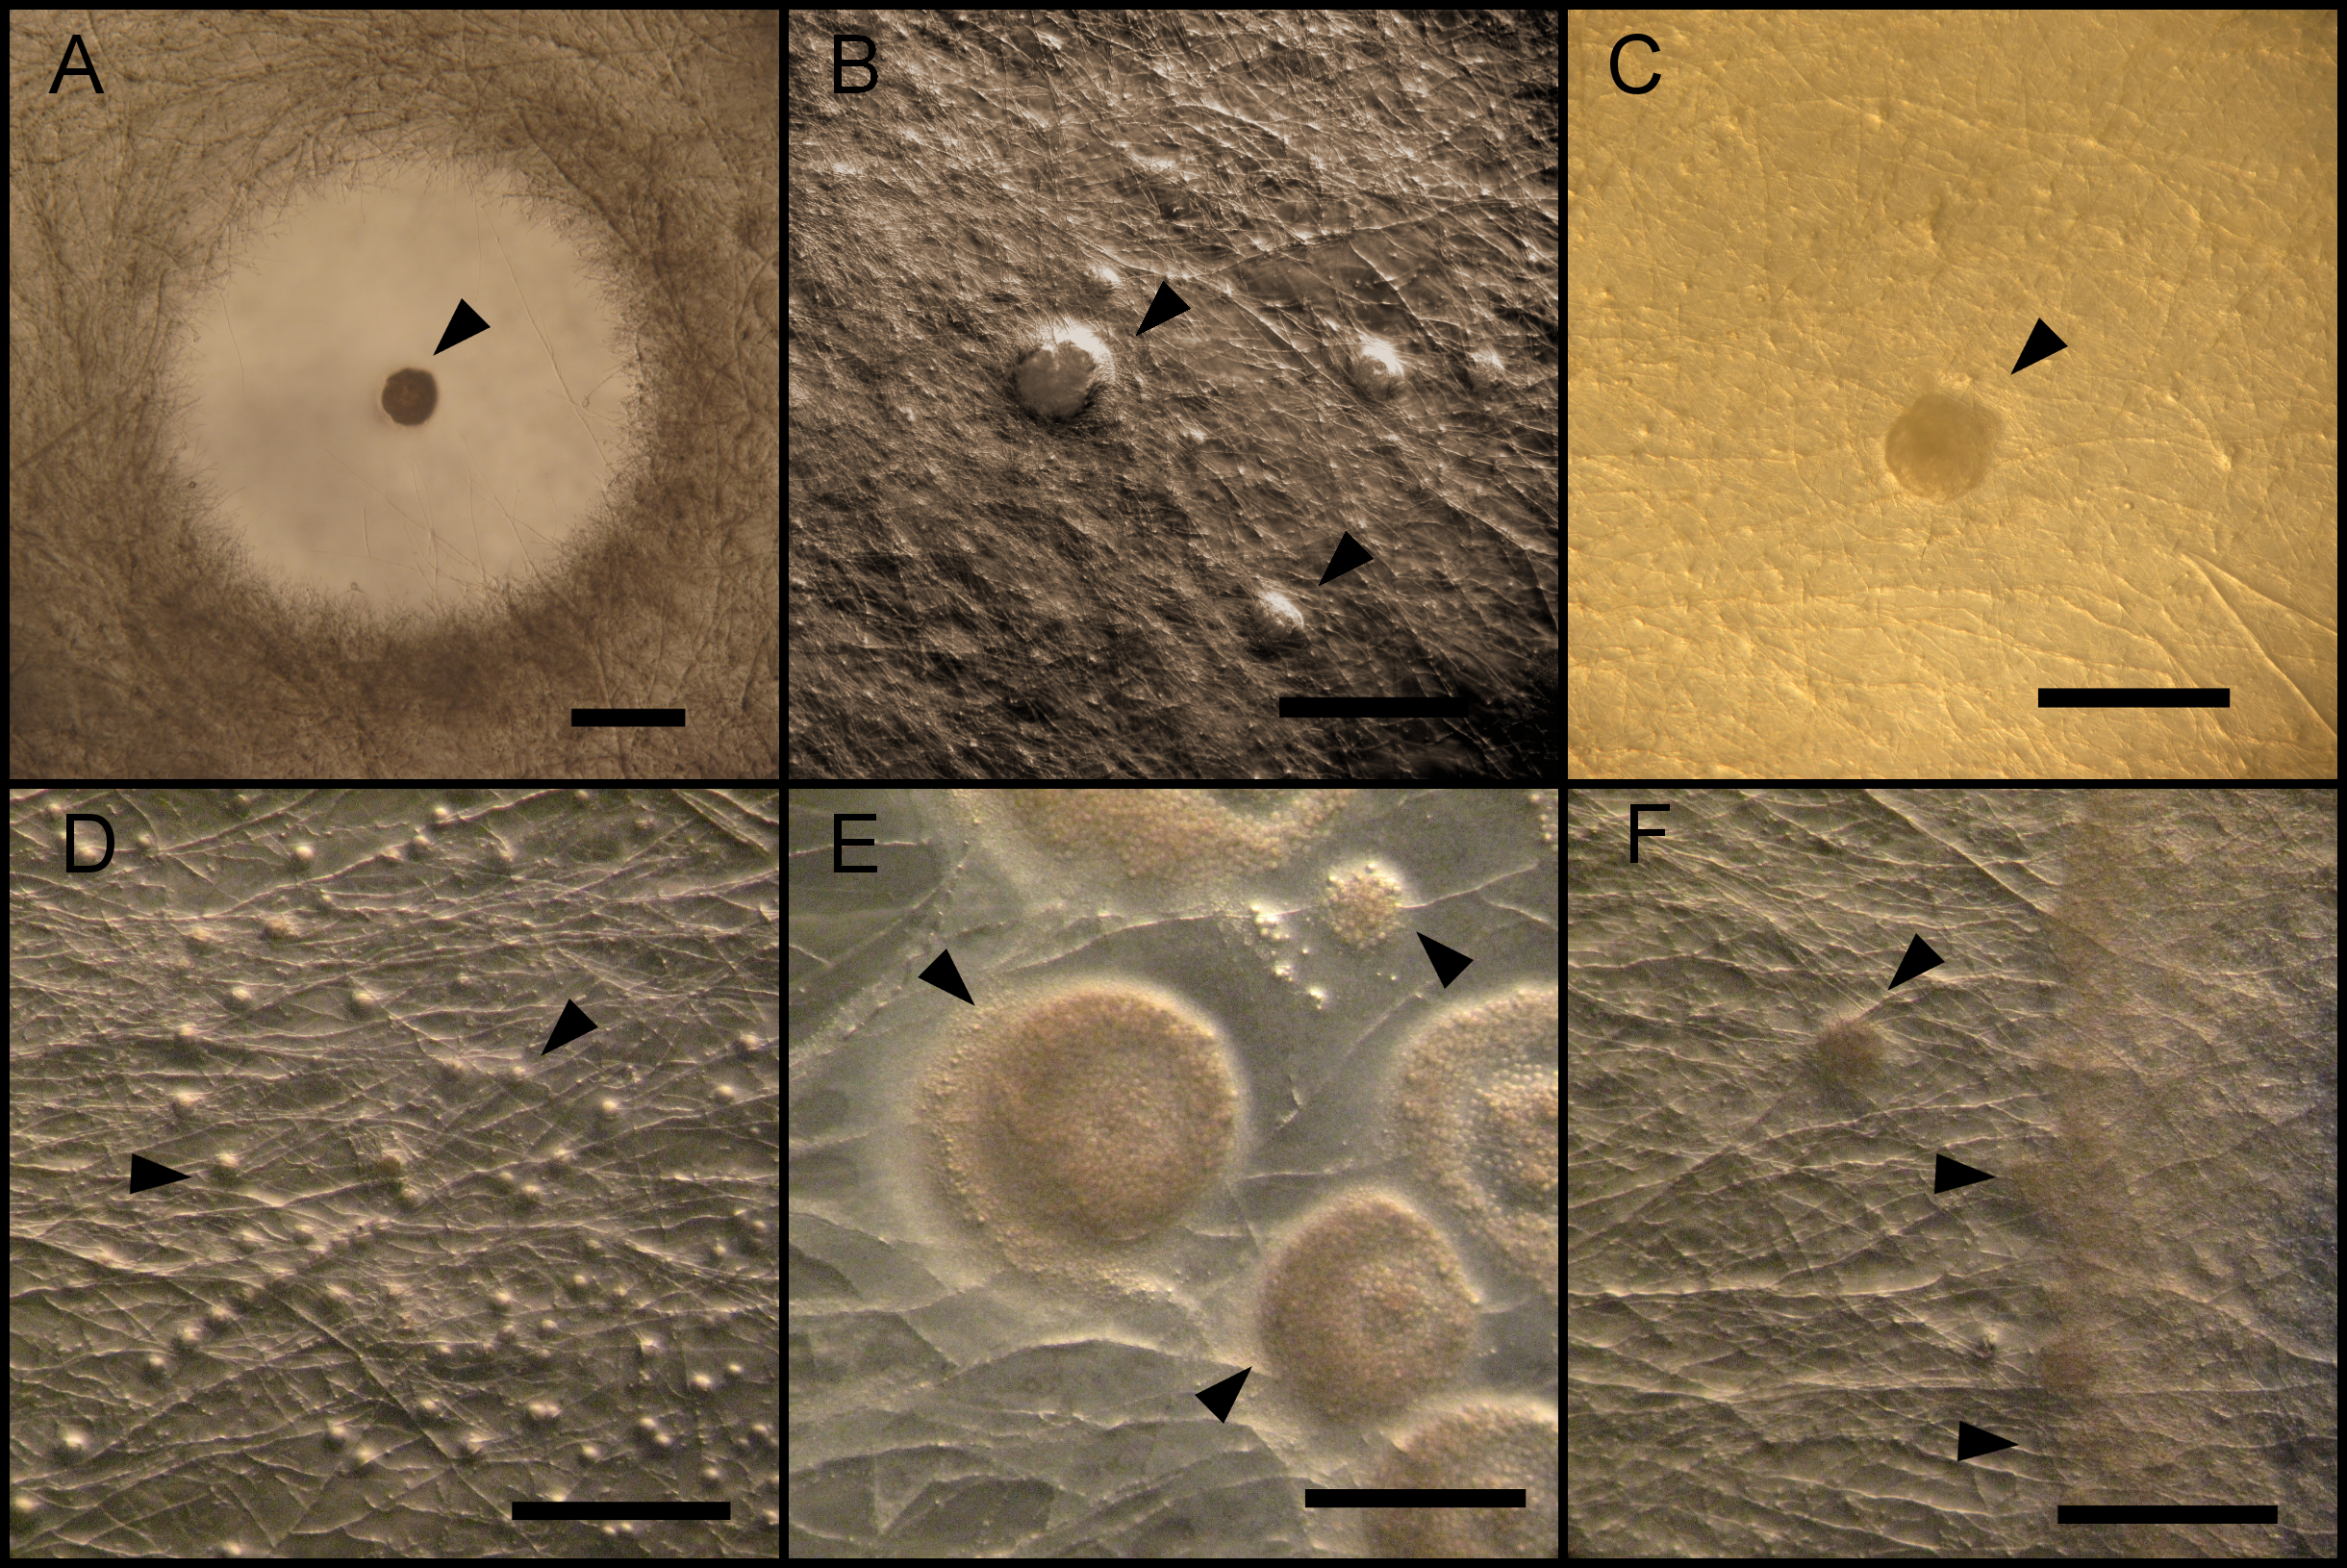
\includegraphics[width=4in]{./Chapter_Inhibition/img/Nc_HpBdSp_otherChytrids.png}
  \caption[Inhibition of \textit{N. crassa} is observed with \textit{H. polyrhiza} and not other chytrids.]{\textit{Batrachochytrium dendrobatidis} JEL 423 (\textit{Bd}), the closest relative of \textit{Hp}, is well known as a global emerging pathogen of amphibians and is the causative agent for recent worldwide amphibian decline. \textit{Spizellomyces punctatus} SW-1 (\textit{Sp}) is a soil saprobe and is not known to be pathogenic. A) \textit{Hp} cultured with \textit{N. crassa} produces a cleared zone. B) \textit{Bd}, C) \textit{Sp}, D) \textit{Operculomyces laminatus} JEL 223, E) \textit{Rhizoclosmatium hyalinus} JEL 800, F) \textit{Obelidium mucronatum} JEL 802 do not display this property. Black scale bars = 1mm. Black arrowheads illustrate location of chytrid sporangia.}
  \label{fig:ChInhib_NcraChytrid}
\end{figure}

\begin{figure}[hb]
  \centering
  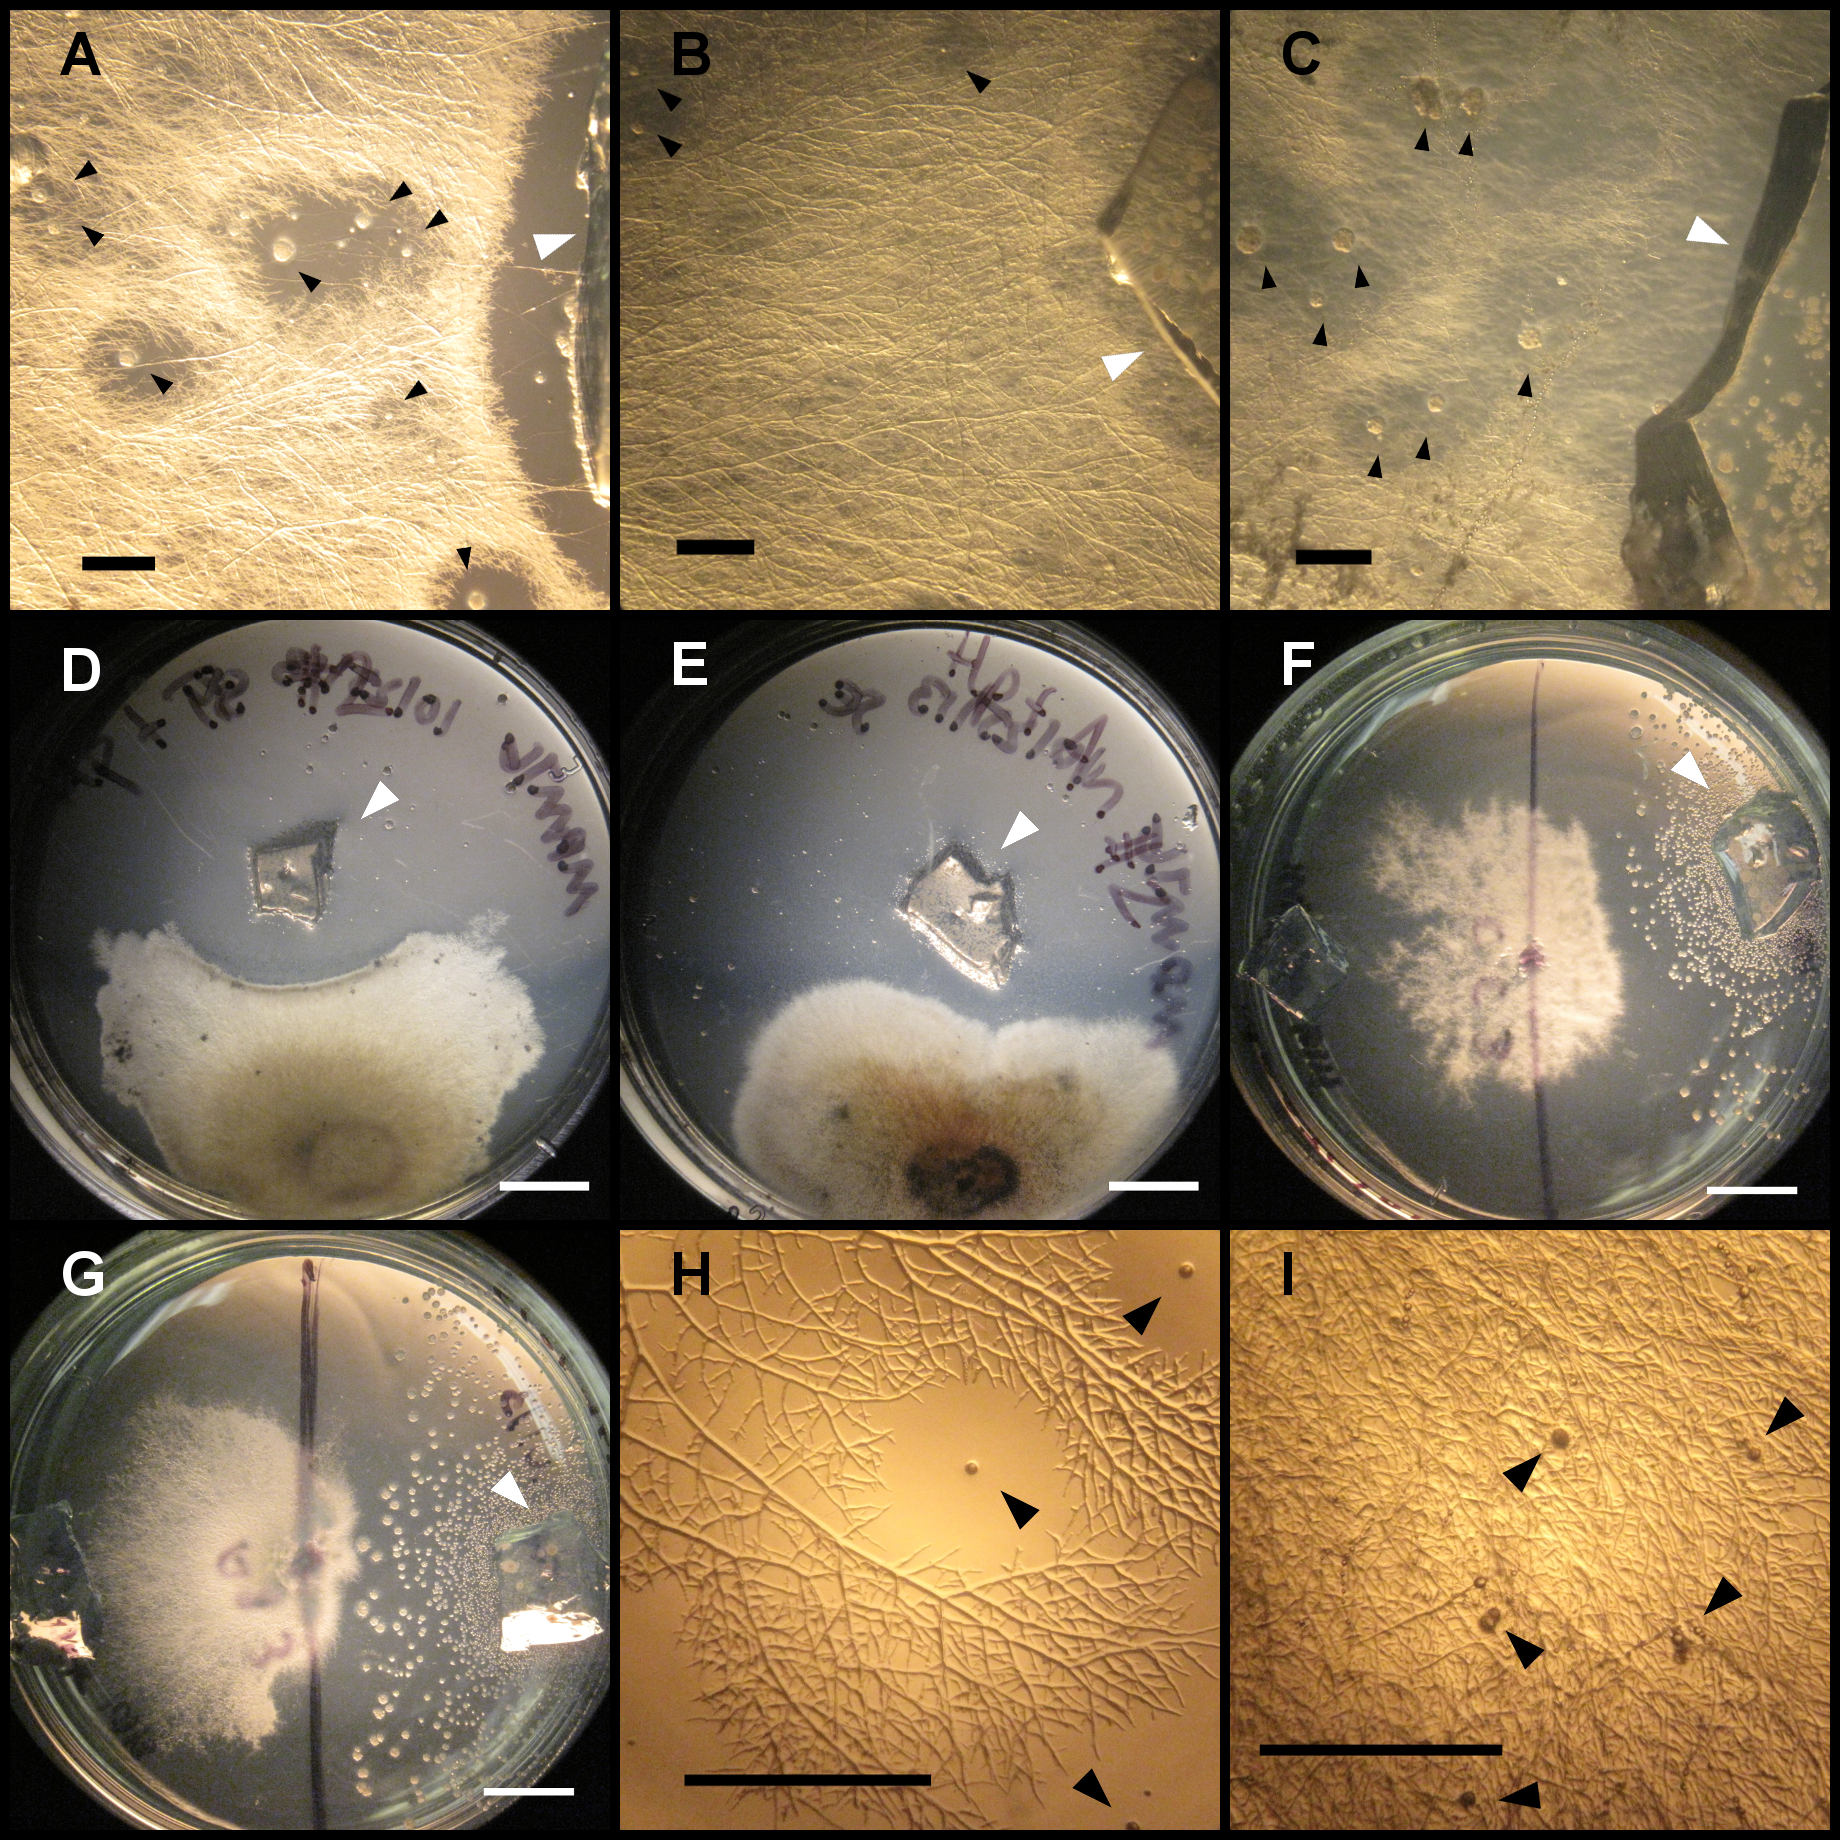
\includegraphics[width=4in]{./Chapter_Inhibition/img/HpvsOtherFungi.png}
  \caption[Inhibitory properties of \textit{H. polyrhiza} are not specific to \textit{N. crassa}.]{A selection of fungal species from the Ascomycota, Basidiomycota, and Mucorales were assayed for sensitivity against \textit{Hp} sporangia. A) \textit{Neurospora crassa} (Sordariomycetes; Sordariales; Sordariaceae), B) \textit{Neurospora tetrasperma}, C) \textit{Neurospora discreta}, D) \textit{Trichoderma reesei} (Sordariomycetes; Hypocreales; Hypocreaceae), E) \textit{Aspergillus nidulans} (Eurotiomycetes; Eurotiales; Trichocomaceae), F) \textit{Coprinopsis cinerea} (Agaricomycetes; Agaricales; Psathyrellaceae), G) \textit{Ashbya gossypii} (Saccharomycetes; Saccharomycetales; Saccharomycetaceae), H) \textit{Phycomyces blakesleeanus} (Mucorales; Phycomycetaceae), and I) \textit{Rhizopus oryzae} (Mucorales; Mucoraceae). Scale bars for A-C,H-I = 1mm. Scale bars for D-G = 5mm. Black arrowheads in A-C,H-I indicate \textit{Hp} sporangia. White arrowheads in A-G indicate blocks of agar with active \textit{Hp} sporangia.}
  \label{fig:ChInhib_HpOtherFungi}
\end{figure}

\begin{figure}[hb]
  \centering
  \includegraphics[width=4in]{./Chapter_Inhibition/img/96h_HpNcColdHotFresh.png}
  \caption[Filter-sterilized \textit{Hp}-conditioned media effectively inhibits \textit{N. crassa} growth.]{Test tubes containing filter-sterilized \textit{Hp}-conditioned media ("filtrate") were inoculated with \textit{N. crassa} conidia and left to incubate at room temperature for 96h (see methods for more detail). For A), B), and C), filtrate was derived from initial preparations of \textit{Hp} alone, \textit{N. crassa} alone, and \textit{Hp}+\textit{N. crassa}, respectively. Panel B) establishes that nutrient limitation is not responsible for inhibitory observation as growth of \textit{N. crassa} can still be supported, while A) and C) establish that \textit{Hp} is not exhibiting this behavior as a response to the presence of another fungus. D), E), F), G) contain \textit{Hp}-derived mPmTG filtrate after low (-20$^{\circ}$C), high (60$^{\circ}$C), ultra-low (-80$^{\circ}$) and ultra-high (90$^{\circ}$) temperature treatments, respectively. For D-G, N. crassa inoculation occurred after media was allowed to return to room temperature. H) \textit{N. crassa} growth in fresh mPmTG media.}
  \label{fig:ChInhib_FilterTempAssay}
\end{figure}

\begin{figure}[hb]
  \centering
  \includegraphics[width=4in]{./Chapter_Inhibition/img/HpBd_pHTempAssay.png}
  \caption[\textit{H. polyrhiza} is more tolerant of environmental stresses than \textit{B. dendrobatidis}.]{A) \textit{Hp} and \textit{Bd} were grown at different pH levels, ranging from 4 to 8. A pH of 6.8 represents the standard pH at which the respective optimal media is prepared. B) \textit{Hp} growth after x days at various temperatures ranging from y$^{\circ}$C to z$^{\circ}$C.}
  \label{fig:ChInhib_HpBdpHTemp}
\end{figure}

\begin{figure}[hb]
  \centering
  \includegraphics[width=4in]{./Chapter_Inhibition/img/HpNc_avoidance.png}
  \caption[\textit{N. crassa} displays no avoidance behavior of solid agar blocks.]{Solid agar plates of mPmTG media containing A) actively growing \textit{H. polyrhiza} and B) no \textit{H. polyrhiza} growth. After 72 hours post-inoculation of \textit{N. crassa}, zones of inhibition are clearly visible surrounding \textit{H. polyrhiza} sporangia. White arrowheads in A and B indicate agar blocks containing or lacking, respectively, \textit{H. polyrhiza} sporangia. Black arrowheads indicate point of inoculation with \textit{N. crassa} conidia. Plates are 100mm in diameter.}
  \label{fig:ChInhib_NcAvoidance}
\end{figure}

%\begin{figure}[hb]
%  \centering
%  \includegraphics[width=4in]{./Chapter_Inhibition/img/Liquid_96hAssay.png}
%  \caption[Liquid 96h assay.]{Hp conditioned media filtrate loses its efficacy after around 96h at room temperature. A) Conditioned media derived from “Hp alone” preparations. B) Conditioned media derived from “Hp+Nc” preparations.}
%  \label{fig:Liquid_96h}
%\end{figure}

%\begin{figure}[hb]
%  \centering
%  \includegraphics[width=4in]{./Chapter_Inhibition/img/yeast_ecoli_filtrate_72h.png}
%  \caption[Growth of yeast and bacterial cultures in liquid media is also inhibited by \textit{Hp} conditioned media.]{OD$_{600}$ measurements of liquid cultures of \textit{S. cerevisiae} MAU99 and AH109, and \textit{E. coli} DH5$\alpha$ after 72h stationary incubation in different media preparations at room temperature: filter-sterilized \textit{Hp}-conditioned media (black), \textit{Hp} liquid mPmTG media (grey), and either liquid YPDA or LB for yeast or \textit{E. coli}, respectively (white).}
%  \label{fig:ChInhib_HpYeastEcoli}
%\end{figure}

%\begin{figure}[hb]
%  \centering
%  \includegraphics[width=4in]{./Chapter_Inhibition/img/Ncra_liquidDilution.png}
%  \caption[\textit{N. crassa} remains susceptible to \textit{H. polyrhiza} conditioned media after dilution]{Filter-sterilized \textit{Hp} conditioned media ("filtrate") was diluted to A) 100\%, B) 50\%, C) 20\% , D) 10\%, and E) 0\% with mPmTG and sterile diH$_{2}$O.}
%  \label{fig:ChInhib_NcraDilution}
%\end{figure}

%\begin{figure}[hb]
%  \centering
%  \includegraphics[width=4in]{./Chapter_Inhibition/img/030915_BdmPmTG_BdFiltrate_on1T_14d.png}
%  \caption[Incubation in \textit{H. polyrhiza} conditioned media prevents encystment and subsequent growth of \textit{B. dendrobatidis} zoospores]{Filter-sterilized \textit{Hp} conditioned media ("filtrate") was used as a growth medium for \textit{B. dendrobatidis} sporangia-containing agar blocks. After a 72hour incubation at room temperature, the liquid suspension was removed and plated on 1\% Tryptone agar plates. Plates were examined after 14d room temperature incubation. Zoospore suspensions were drawn from A) filtrate preparations and B) fresh mPmTG preparations.}
%  \label{fig:ChInhib_HpvsBd}
%\end{figure}

%%%%%%%%%%%%%%%%%%%%%%%%%%%%%%%%%%%%%%%%%%%%%%%%%%%%%%%%%%%%%%%%%%%%%%%
%% Document: Thesis for PhD at UC Riverside                          %%
%% Description: A comparative analysis of environment sensing in EDF %%
%% Author: Steven Ahrendt                                            %%
%%%%%%%%%%%%%%%%%%%%%%%%%%%%%%%%%%%%%%%%%%%%%%%%%%%%%%%%%%%%%%%%%%%%%%%
% INHIBITION TABLES %
%%%%%%%%%%%%%%%%%%%%%

% Kinase Mutant Screen
% latex table generated in R 3.0.1 by xtable 1.7-4 package
% Sun May 24 12:52:01 2015
\begin{table}[ht]
\centering
\caption{Kinase and phosphotase mutants used in screening against \textit{H. polyrhiza} sporangia.} 
\label{tab:ChInhib_Kinase}
\begin{tabular}{lllll}
  \hline
Mutant & Group & Family & NCU & Neurospora\_gene \\ 
  \hline
x1 & pp2A & - & - & - \\ 
  x2 & ppt-1 & - & - & - \\ 
  x3 & CMGC & MAPK & NCU07024 & os-2 \\ 
  x4 & STE & STE11 & NCU03071 & os-4 \\ 
  x5 & STE & STE7 & NCU00587 & os-5 \\ 
  1846 & CAMK & CAMKL & NCU00914 & stk-16 \\ 
  1849 & Other & PEK & NCU01187 & cpc-3 \\ 
  1885 & STE & STE20 & NCU03894 & stk-4 \\ 
  1888 & Other & WEE & NCU04326 & stk-29 \\ 
  1916 & Unclassified & - & NCU06421 & stk-41 \\ 
  1917 & Unclassified & - & NCU06422 & stk-42 \\ 
  1919 & Unclassified & - & NCU06583 & stk-44 \\ 
  1920 & Other & VPS15 & NCU06626 & stk-45 \\ 
  1925 & AGC & YANK & NCU07062 & stk-49 \\ 
  1936 & CGMC & CLK/SRPK & NCU10004 & stk-56 \\ 
  1937 & Unclassified & - & NCU05638 & stk-34 \\ 
  1944 & CMGC & CDK & NCU07880 & prk-6 \\ 
  1946 & Other & IKS & NCU08177 & stk-51 \\ 
  2294 & CAMK & CAMKL & NCU04747 & stk-31 \\ 
   \hline
\end{tabular}
\end{table}
% Chytrid secretome
% latex table generated in R 3.0.1 by xtable 1.7-4 package
% Sun May 24 12:52:01 2015
\begin{table}[ht]
\centering
\caption[Chytrid secretome predictions]{Proteins predicted to be in the secretome of basal fungi} 
\label{tab:ChInhib_ChySec}
\begin{tabular}{rr}
  \hline
 & Num of proteins \\ 
  \hline
R. allomycis &  32 \\ 
  G. prolifera & 101 \\ 
  Piromyces E2 & 269 \\ 
  Orpinomyces C1 & 280 \\ 
  H. polyrhiza &  58 \\ 
  S. punctatus &  66 \\ 
  B. dendrobatidis & 133 \\ 
  A. macrogynus &  57 \\ 
  C. anguillulae & 101 \\ 
  C. lativittatus &  98 \\ 
   \hline
\end{tabular}
\end{table}

%%%%%%%%%%%%%%%
% CONCLUSIONS %
%%%%%%%%%%%%%%%
%%%%%%%%%%%%%%%%%%%%%%%%%%%%%%%%%%%%%%%%%%%%%%%%%%%%%%%%%%%%%%%%%%%%%%%%%%%%%%%%%
%% Document: Thesis for PhD at UC Riverside                                    %%
%% Title: Investigating the evolution of environmental and biotic interactions %%
%%          in basal fungal lineages through comparative genomics              %%
%% Author: Steven Ahrendt                                                      %%
%%%%%%%%%%%%%%%%%%%%%%%%%%%%%%%%%%%%%%%%%%%%%%%%%%%%%%%%%%%%%%%%%%%%%%%%%%%%%%%%%
% CONCLUSIONS %
%%%%%%%%%%%%%%%
\chapter{Conclusions}
\section{Background}
The objective of this research was to enhance the current knowledge about early-diverging fungal groups. More and more reasearchers are turning towards these organisms as afocal points for study as they occupy a unique position between the fungal-animal common ancestor, and the more popular and accessible fungal research systems (ie Ascomycota and Basidiomycota model organisms). Additionally, genomic resources and methodologies are becoming increasingly more accessible, and so the ability to incorporate this data into existing studies is becomign more widespread.\\
\section{Aims}
The aims for this dissertation research were:\\
\begin{enumerate}
  \item Characterize the identification of an opsin-like protein
  \item Describe and identify a compopund responsible for antifungal behavior
  \item Produce and interpret a transcriptome for mosquito pathogen; lay groundwork for enhanced genomic resources
\end{enumerate}



%%%%%%%%%%%%%%%%
% BIBLIOGRAPHY %
%%%%%%%%%%%%%%%%
%\nocite{*}
% \singlespacing
%\bibliographystyle{alpha} % Alphabetical 
%\bibliographystyle{plain} % default in UCR template
\bibliographystyle{ieeetr} % this style lists refs in order of appearance
\bibliography{Ahrendt_thesisRefs}

%%%%%%%%%%%%
% APPENDIX %
%%%%%%%%%%%%
\appendix
%%%%%%%%%%%%%%%%%%%%%%%%%%%%%%%%%%%%%%%%%%%%%%%%%%%%%%%%%%%%%%%%%%%%%%%%%%%%%%%%%
%% Document: Thesis for PhD at UC Riverside                                    %%
%% Title: Investigating the evolution of environmental and biotic interactions %%
%%          in basal fungal lineages through comparative genomics              %%
%% Author: Steven Ahrendt                                                      %%
%%%%%%%%%%%%%%%%%%%%%%%%%%%%%%%%%%%%%%%%%%%%%%%%%%%%%%%%%%%%%%%%%%%%%%%%%%%%%%%%%
%% FLAGELLAR ANALYSIS %
%%%%%%%%%%%%%%%%%%%%%%%
\chapter{Comparative genomics analysis of Flagellar motility}
\label{app:Flagella}
\section{Introduction}
\section{Results and Discussion}
A search for Rozella homologs of flagellar-associated proteins from the \textit{Naeglaria} genome \cite{FritzLaylin2011} reveal a pattern of presence/absence of proteins in Rozella which correlates with that found in the Chytridiomycota and Blastocladiomycota. This pattern, in general, differs from the Microsporidia, supporting the placement of Rozella as prior to the Chytridiomycota/Blastocladiomycota and a flagellar loss event after the divergence of the Microsporidia. \\
\indent (Figure~\ref{fig:AppFlag_heatmap}).\\
\section{Methods}
The flagellar analysis was carried out using a dataset of 173 flagellar motility proteins obtained from the \textit{Naeglaria grubeii} genome sequence \cite{FritzLaylin2011}. These proteins were used in a FASTA search (SSEARCH v36.07) using an e-val cutoff of e-20. Supplemental table X only considers proteins which are present in at least one Dikarya, Microsporidia, or Chytridiomycota proteom. PSI-BLAST \cite{Altschul1997} was used to identify homologs of the three polar-tube proteins (PTP1, PTP2, and PTP3) characterized previously [PMIDs: 11719806, 12076771].\\

%%%%%%%%%%%%%%%%%%%%%%%%%%%%%%%%%%%%%%%%%%%%%%%%%%%%%%%%%%%%%%%%%%%%%%%%%%%%%%%%%
%% Document: Thesis for PhD at UC Riverside                                    %%
%% Title: Investigating the evolution of environmental and biotic interactions %%
%%          in basal fungal lineages through comparative genomics              %%
%% Author: Steven Ahrendt                                                      %%
%%%%%%%%%%%%%%%%%%%%%%%%%%%%%%%%%%%%%%%%%%%%%%%%%%%%%%%%%%%%%%%%%%%%%%%%%%%%%%%%%
%% APPENDIX FIGURES %%
%%%%%%%%%%%%%%%%%%%%%%

% Flagellar heat map from James et al 2009
\begin{figure}
  \centering
  \includegraphics[width=4in]{./Appendix/img/flagDataHeatmap.png}
  \caption[Heatmap cluster analysis of flagellar proteins from \textit{Naegleria gruberi}]{Protein copies identified in proteomes of interest are normalized to indicate presence and absence only, where green indicates that one or more copies were found. Proteins are listed on the right, and proteomes given on the bottom. Both rows and columns are clustered by the "complete" method}
  \label{fig:AppFlag_heatmap}
\end{figure}

%%%%%%%%%%%%%%%%%%%%%%%%%%%%%%%%%%%%%%%%%%%%%%%%%%%%%%%%%%%%%%%%%%%%%%%%%%%%%%%%%
%% Document: Thesis for PhD at UC Riverside                                    %%
%% Title: Investigating the evolution of environmental and biotic interactions %%
%%          in basal fungal lineages through comparative genomics              %%
%% Author: Steven Ahrendt                                                      %%
%%%%%%%%%%%%%%%%%%%%%%%%%%%%%%%%%%%%%%%%%%%%%%%%%%%%%%%%%%%%%%%%%%%%%%%%%%%%%%%%%
%% MISC DATA USED IN THESIS %%
%%%%%%%%%%%%%%%%%%%%%%%%%%%%%%
\chapter{Datasets and scripts}
\label{app:Data}
\section*{Datasets}
A list of proteomes from each organisms, the source website, and version used in these analyses is provided in Table~\ref{tab:AppData_taxa}.\\
A table of the PDB IDs used in the structural modeling, docking, and MD simulations presented in Chapter~\ref{chap:RhodStruct} are provided in Table~\ref{tab:AppData_PDB}.\\
Sequences used in \textit{Pichia pastoris} cloning, described in Chapter~\ref{chap:RhodAux}, are given here:\\
\VerbatimInput{./Appendix/dat/PichiaExpressionSequences.fasta}
\section*{Scripts}
All scripts are available on github: \url{https://github.com/stajichlab/ahrendt_thesis/tree/master/Scripts}

%%%%%%%%%%%%%%%%%%%%%%%%%%%%%%%%%%%%%%%%%%%%%%%%%%%%%%%%%%%%%%%%%%%%%%%%%%%%%%%%%
%% Document: Thesis for PhD at UC Riverside                                    %%
%% Title: Investigating the evolution of environmental and biotic interactions %%
%%          in basal fungal lineages through comparative genomics              %%
%% Author: Steven Ahrendt                                                      %%
%%%%%%%%%%%%%%%%%%%%%%%%%%%%%%%%%%%%%%%%%%%%%%%%%%%%%%%%%%%%%%%%%%%%%%%%%%%%%%%%%
%% MISC LIST OF DATA %%
%%%%%%%%%%%%%%%%%%%%%%%

% Taxa and sources
% latex table generated in R 3.1.1 by xtable 1.7-3 package
% Mon Jun 22 14:41:00 2015
{\renewcommand{\arraystretch}{0.5}
{\footnotesize
{\setlength{\tabcolsep}{1pt}
\begin{longtable}{rllrlll}
\caption[List of proteomes used in comparative analyses.]{List of all proteomes used in comparative analyses, including NCBI taxonomy database ID, phylogenetic abbreviation ("Key"), phylum designation ("Group"), isolate number/version (where applicable), and source website.} \label{tab:AppData_taxa} \\
  \hline
\hline
 & Key & Group & TaxID & Name & Isolate/Version & Reference \\ 
  \hline
Aben & APF & Ascomycota & 663331 & \emph{Arthroderma benhamiae} & CBS 112371 & \cite{Dermato} \\ 
  Afum & AEF & Ascomycota & 746128 & \emph{Aspergillus fumigatus} & Af293 & \cite{Nierman2005} \\ 
  Agos & ASaF & Ascomycota & 33169 & \emph{Ashbya gossypii} & ATCC 10895 v1.0 & \cite{Dietrich2004} \\ 
  Aloc & MF & Microsporidia & 278021 & \emph{Antonospora locustae} & HM-2013 v1.0 & \cite{Slamovits2004,Corradi2007} \\ 
  Amac & CBF & Chytrids & 28583 & \emph{Allomyces macrogynus} & ATCC 38327 & \cite{RuizTrillo2007} \\ 
  Anid & AEF & Ascomycota & 227321 & \emph{Aspergillus nidulans} & FGSC A4 & \cite{Galagan2005} \\ 
  Bcin & ALoF & Ascomycota & 332648 & \emph{Botrytis cinerea} & B05.10 & \cite{Amselem2011} \\ 
  Bcir & ZMF & Zygomycota & 1314798 & \emph{Backusella circina} & FSU 941 & \cite{Bcir} \\ 
  Bde2 & CCF & Chytrids & 684364 & \emph{Batrachochytrium dendrobatidis} & JAM 81 v1.0 & \cite{Bde2} \\ 
  Bden & CCF & Chytrids & 403673 & \emph{Batrachochytrium dendrobatidis} & JEL 423 & \cite{Bden} \\ 
  Bder & AEF & Ascomycota & 559298 & \emph{Blastomyces dermatitidis} & SLH14081 & \cite{McCullough2000} \\ 
  Beme & CBF & Chytrids & 4808 & \emph{Blastocladiella emersonii} & --- & \cite{Ribichich2005} \\ 
  Cang & CBF & Chytrids & 109876 & \emph{Catenaria anguillulae} & PL171 v1.0 & \cite{Cang} \\ 
  Ccin & BAF & Basidiomycota & 5346 & \emph{Coprinopsis cinerea} & okayama7\_130 & \cite{Stajich2010Ccin} \\ 
  Ccor & ZEF & Zygomycota & 34488 & \emph{Conidiobolus coronatus} & NRRL28638 v1.0 & \cite{Chang2015} \\ 
  Cimm & AEF & Ascomycota & 246410 & \emph{Coccidioides immitis} & RS & \cite{Sharpton2009} \\ 
  Cint & OA & Animal & 7719 & \emph{Ciona intestinalis} & v2.0 & \cite{Cint} \\ 
  Clat & CBF & Chytrids & 945690 & \emph{Coelomomyces lativittatus} & --- & --- \\ 
  Cmer & OAO & OAO & 45157 & \emph{Cyanidioschyzon merolae} & 10D v1.0 & \cite{Matsuzaki2004} \\ 
  Cneo & BAF & Basidiomycota & 5207 & \emph{Cryptococcus neoformans} & \textit{var. grubii} H99 & \cite{Cneo} \\ 
  Cowc & OA & Animal & 192875 & \emph{Capsaspora owczarzaki} & ATCC 30864 & \cite{RuizTrillo2007} \\ 
  Crei & OP & Viridiplantae & 3055 & \emph{Chlamydomonas reinhardtii} & v4.0 & \cite{Merchant2007} \\ 
  Crev & ZF & Zygomycota & 61392 & \emph{Coemansia reversa} & NRRL 1564 v1.0 & \cite{Chang2015} \\ 
  Daci & ADF & Ascomycota & 112489 & \emph{Dissoconium aciculare} & CBS 342.82 v1.0 & \cite{Daci} \\ 
  Dbis & BAF & Basidiomycota & 1314803 & \emph{Dendrothele bispora} & CBS 962.96 v1.0 & \cite{Dbis} \\ 
  Ddis & OAM & Amoebozoa & 44689 & \emph{Dictyostelium discoideum} & --- & \cite{Eichinger2005} \\ 
  Dmel & OA & Metazoa & 7227 & \emph{Drosophila melanogaster} & v5 & \cite{DosSantos2015} \\ 
  Dsym & ADF & Ascomycota & 548649 & \emph{Dothidotthia symphoricarpi} & CBS 119687 v1.0 & \cite{Dsym} \\ 
  Ebie & MF & Microsporidia & 31281 & \emph{Enterocytozoon bieneusi} & H348 & \cite{Corradi2007} \\ 
  Ecun & MF & Microsporidia & 6035 & \emph{Encephalitozoon cuniculi} & GB-M1 & \cite{Micro} \\ 
  Eint & MF & Microsporidia & 58839 & \emph{Encephalitozoon intestinalis} & ATCC 50506 & \cite{Micro} \\ 
  Falb & OAM & Amoebozoa & 691883 & \emph{Fonticula alba} & ATCC 38817 v2.0 & \cite{RuizTrillo2007} \\ 
  Fgra & ASoF & Ascomycota & 229533 & \emph{Fusarium graminearum } & PH-1 & \cite{Fgra} \\ 
  Gpro & CF & Chytrids & 1123529 & \emph{Gonapodya prolifera} & JEL478 v1.0 & \cite{Chang2015} \\ 
  Hmag & OA & Animal & 6085 & \emph{Hydra magnipapillata} & strain 105 & \cite{Chapman2010} \\ 
  Hpol & CCF & Chytrids & 166479 & \emph{Homolaphlyctis polyrhiza} & JEL 142 & --- \\ 
  Lhya & ZF & Zygomycota & 420593 & \emph{Lichtheimia hyalospora} & v1.0 & \cite{Lhya} \\ 
  Lmac & ADF & Ascomycota & 372055 & \emph{Lophiostoma macrostomum} & CBS 122681 v1.0 & \cite{Lmac} \\ 
  Mani & ASoF & Ascomycota & 5530 & \emph{Metarhizium anisopliae} & ARSEF 23 v1.0 & \cite{Gao2011} \\ 
  Mbre & OA & Animal & 81824 & \emph{Monosiga brevicollis} & MX1 & \cite{RuizTrillo2007} \\ 
  Mcan & AEF & Ascomycota & 554155 & \emph{Microsporum canis} & CBS 113480 & \cite{Dermato} \\ 
  Mcir & ZMF & Zygomycota & 36080 & \emph{Mucor circinelloides} & f. sp. \emph{circinelloides} & \cite{Lee2014} \\ 
  Mver & ZMF & Zygomycota & 78898 & \emph{Mortierella verticillata} & NRRL 6337 & \cite{RuizTrillo2007} \\ 
  Ncer & MF & Microsporidia & 40302 & \emph{Nosema ceranae} & BRL01 v1.0 & \cite{Cornman2009} \\ 
  Ncra & ASoF & Ascomycota & 5141 & \emph{Neurospora crassa} & OR74A & \cite{Ncra} \\ 
  Npar & MF & Microsporidia & 586133 & \emph{Nematocida parisii} & ERTm1 & \cite{Cuomo2012} \\ 
  Npha & OAR & Archaea & 348780 & \emph{Natromonas pharaonis} & DSM 2160 & \cite{Falb2005} \\ 
  OrpC & CNF & Chytrids & 1117330 & \emph{Orpinomyces} sp & C1A & \cite{Youssef2013} \\ 
  Patr & ADF & Ascomycota & 703506 & \emph{Patellaria atrata} & CBS 101060 v1.0 & \cite{Patr} \\ 
  Pbla & ZMF & Zygomycota & 4837 & \emph{Phycomyces blakesleeanus} & NRRL1555,v2.0.JGI & \cite{Pbla} \\ 
  Pgra & BPF & Basidiomycota & 418459 & \emph{Puccinia graminis f.sp. tritici} & CRL75-36-700-3 & \cite{Pgra} \\ 
  PirE & CNF & Chytrids & 45796 & \emph{Piromyces} sp & E2 v1.0 & \cite{PirE} \\ 
  Psip & ADF & Ascomycota & 100044 & \emph{Pleomassaria siparia} & CBS 279.74 & \cite{Psip} \\ 
  Psoj & OAO & Stramenopiles & 67593 & \emph{Phytophthora sojae} & v3.0 & \cite{Tyler2006} \\ 
  Ptri & ADF & Ascomycota & 426418 & \emph{Pyrenophora tritici-repentis} & Pt-1C-BFP & \cite{Manning2013} \\ 
  Pult & OAO & OAO & 431595 & \emph{Pythium ultimum} & DAOM BR144,v.2010-07-12 & \cite{Levesque2010} \\ 
  Rall & MF & Cryptomycota & 281847 & \emph{Rozella allomycis} & v.2012-05-03 & \cite{James2013} \\ 
  Rirr & ZMF & Zygomycota & 588596 & \emph{Rhizophagus irregularis} & DAOM 181602 & \cite{Tisserant2013} \\ 
  Rmic & ZMF & Zygomycota & 58291 & \emph{Rhizopus microsporus} & var \emph{microsporus} ATCC52813 v1.0 & \cite{Rmic} \\ 
  Rory & ZMF & Zygomycota & 64495 & \emph{Rhizopus oryzae} & 99-880,v.1 & \cite{Ma2009} \\ 
  Sarc & OA & Animal & 72019 & \emph{Sphaeroforma arctica } & JP610 & \cite{RuizTrillo2007} \\ 
  Scer & ASaF & Ascomycota & 4932 & \emph{Saccharomyces cerevisiae} & S288C, v.2011-02-03 & \cite{Scer} \\ 
  Sfim & ADF & Ascomycota & 718229 & \emph{Sporormia fimetaria} & CBS 119925 v1.0 & \cite{Sfim} \\ 
  Spom & ATF & Ascomycota & 4896 & \emph{Schizosaccharomyces pombe} & v.20 & \cite{Wood2002} \\ 
  Spun & CCF & Chytrids & 109760 & \emph{Spizellomyces punctatus} & DAOM BR117 & \cite{RuizTrillo2007} \\ 
  Sros & BF & Basidiomycota & 40563 & \emph{Sporobolomyces roseus} & v1.0 & \cite{Sros} \\ 
  Srot & OA & Animal & 946362 & \emph{Salpingoeca rosetta} & ATCC 50818 & \cite{RuizTrillo2007} \\ 
  Sscl & ALoF & Ascomycota & 665079 & \emph{Sclerotinia sclerotiorum} & 1980\_UF-70.30,v.2009-01.Broad & \cite{Sscl} \\ 
  Tgon & OAP & Apicomplexian & 5811 & \emph{Toxoplasma gondii} & ME49,v.2008-07-23.ToxoDB-7.2 & \cite{Kissinger2003} \\ 
  Tpse & OAO & OAO & 35128 & \emph{Thalassiosira pseudonana} & CCMP1335,v.JGI3 & \cite{Armbrust2004} \\ 
  Trub & AEF & Ascomycota & 559305 & \emph{Trichophyton rubrum} & CBS 118892 & \cite{Dermato} \\ 
  Ttra & OA & Animal & 529818 & \emph{Thecamonas trahens} & ATCC 50062 & \cite{RuizTrillo2007} \\ 
  Umay & BUF & Basidiomycota & 5270 & \emph{Ustilago maydis} & v.2011-05-24.MIPS & \cite{Kamper2006} \\ 
  Uram & ZMF & Zygomycota & 41833 & \emph{Umbelopsis ramanniana} & AG v1.0 & \cite{Uram} \\ 
  Uree & AEF & Ascomycota & 336963 & \emph{Uncinocarpus reesii} & UAMH 1704 & \cite{Sharpton2009} \\ 
  Vcul & MF & Microsporidia & 103449 & \emph{Vavraia culicis} floridensis & v.1.Broad & \cite{Micro} \\ 
  Wseb & BAF & Basidiomycota & 148960 & \emph{Wallemia sebi} & CBS-633.66,v.JGI1 & \cite{Padamsee2012} \\ 
  Ylip & ASaF & Ascomycota & 4952 & \emph{Yarrowia lipolytica} & CLIB122,v.14-APR-2010 & \cite{Dujon2004} \\ 
  Zrhi & ADF & Ascomycota & 1314779 & \emph{Zopfia rhizophilia} & CBS 207.26 v1.0 & \cite{Zrhi} \\ 
   \hline
\hline
\end{longtable}
} %horizontal spacing
} %footnote size
} %vertical spacing

% PDB IDs
% latex table generated in R 3.1.1 by xtable 1.7-3 package
% Mon Jun 22 14:41:00 2015
\begin{table}[bp]
\caption[PDB IDs and descriptions of structures used in comparative analyses]{PDB IDs and descriptions of structures used in docking and Molecular dynamics simulations} 
\label{tab:AppData_PDB}
\begin{tabular}{rll}
  \hline
\hline
 PDBID & Description & Reference\\ 
  \hline
 1U19 & Crystal structure of Bovine rhodopsin at 2.2 angstroms resolution & \cite{Okada2004} \\ 
 2Z73 & Crystal structure of Squid rhodopsin & \cite{Murakami2008} \\ 
 1H68 & Sensory rhodopsin II & \cite{Royant2001} \\ 
   \hline
\hline
\end{tabular}

\end{table}

\end{document}
